% Options for packages loaded elsewhere
\PassOptionsToPackage{unicode}{hyperref}
\PassOptionsToPackage{hyphens}{url}
\PassOptionsToPackage{dvipsnames,svgnames,x11names}{xcolor}
%
\documentclass[
  11pt,
]{krantz}
\usepackage{amsmath,amssymb}
\usepackage{lmodern}
\usepackage{iftex}
\ifPDFTeX
  \usepackage[T1]{fontenc}
  \usepackage[utf8]{inputenc}
  \usepackage{textcomp} % provide euro and other symbols
\else % if luatex or xetex
  \usepackage{unicode-math}
  \defaultfontfeatures{Scale=MatchLowercase}
  \defaultfontfeatures[\rmfamily]{Ligatures=TeX,Scale=1}
  \setmonofont[Scale=0.775]{MesloLGS NF}
\fi
% Use upquote if available, for straight quotes in verbatim environments
\IfFileExists{upquote.sty}{\usepackage{upquote}}{}
\IfFileExists{microtype.sty}{% use microtype if available
  \usepackage[]{microtype}
  \UseMicrotypeSet[protrusion]{basicmath} % disable protrusion for tt fonts
}{}
\makeatletter
\@ifundefined{KOMAClassName}{% if non-KOMA class
  \IfFileExists{parskip.sty}{%
    \usepackage{parskip}
  }{% else
    \setlength{\parindent}{0pt}
    \setlength{\parskip}{6pt plus 2pt minus 1pt}}
}{% if KOMA class
  \KOMAoptions{parskip=half}}
\makeatother
\usepackage{xcolor}
\IfFileExists{xurl.sty}{\usepackage{xurl}}{} % add URL line breaks if available
\IfFileExists{bookmark.sty}{\usepackage{bookmark}}{\usepackage{hyperref}}
\hypersetup{
  pdftitle={Data Science per psicologi},
  pdfauthor={Corrado Caudek},
  colorlinks=true,
  linkcolor={Maroon},
  filecolor={Maroon},
  citecolor={Blue},
  urlcolor={Blue},
  pdfcreator={LaTeX via pandoc}}
\urlstyle{same} % disable monospaced font for URLs
\usepackage{color}
\usepackage{fancyvrb}
\newcommand{\VerbBar}{|}
\newcommand{\VERB}{\Verb[commandchars=\\\{\}]}
\DefineVerbatimEnvironment{Highlighting}{Verbatim}{commandchars=\\\{\}}
% Add ',fontsize=\small' for more characters per line
\usepackage{framed}
\definecolor{shadecolor}{RGB}{248,248,248}
\newenvironment{Shaded}{\begin{snugshade}}{\end{snugshade}}
\newcommand{\AlertTok}[1]{\textcolor[rgb]{0.33,0.33,0.33}{#1}}
\newcommand{\AnnotationTok}[1]{\textcolor[rgb]{0.37,0.37,0.37}{\textbf{\textit{#1}}}}
\newcommand{\AttributeTok}[1]{\textcolor[rgb]{0.61,0.61,0.61}{#1}}
\newcommand{\BaseNTok}[1]{\textcolor[rgb]{0.06,0.06,0.06}{#1}}
\newcommand{\BuiltInTok}[1]{#1}
\newcommand{\CharTok}[1]{\textcolor[rgb]{0.5,0.5,0.5}{#1}}
\newcommand{\CommentTok}[1]{\textcolor[rgb]{0.37,0.37,0.37}{\textit{#1}}}
\newcommand{\CommentVarTok}[1]{\textcolor[rgb]{0.37,0.37,0.37}{\textbf{\textit{#1}}}}
\newcommand{\ConstantTok}[1]{\textcolor[rgb]{0,0,0}{#1}}
\newcommand{\ControlFlowTok}[1]{\textcolor[rgb]{0.27,0.27,0.27}{\textbf{#1}}}
\newcommand{\DataTypeTok}[1]{\textcolor[rgb]{0.27,0.27,0.27}{#1}}
\newcommand{\DecValTok}[1]{\textcolor[rgb]{0.06,0.06,0.06}{#1}}
\newcommand{\DocumentationTok}[1]{\textcolor[rgb]{0.37,0.37,0.37}{\textbf{\textit{#1}}}}
\newcommand{\ErrorTok}[1]{\textcolor[rgb]{0.14,0.14,0.14}{\textbf{#1}}}
\newcommand{\ExtensionTok}[1]{#1}
\newcommand{\FloatTok}[1]{\textcolor[rgb]{0.06,0.06,0.06}{#1}}
\newcommand{\FunctionTok}[1]{\textcolor[rgb]{0,0,0}{#1}}
\newcommand{\ImportTok}[1]{#1}
\newcommand{\InformationTok}[1]{\textcolor[rgb]{0.37,0.37,0.37}{\textbf{\textit{#1}}}}
\newcommand{\KeywordTok}[1]{\textcolor[rgb]{0.27,0.27,0.27}{\textbf{#1}}}
\newcommand{\NormalTok}[1]{#1}
\newcommand{\OperatorTok}[1]{\textcolor[rgb]{0.43,0.43,0.43}{\textbf{#1}}}
\newcommand{\OtherTok}[1]{\textcolor[rgb]{0.37,0.37,0.37}{#1}}
\newcommand{\PreprocessorTok}[1]{\textcolor[rgb]{0.37,0.37,0.37}{\textit{#1}}}
\newcommand{\RegionMarkerTok}[1]{#1}
\newcommand{\SpecialCharTok}[1]{\textcolor[rgb]{0,0,0}{#1}}
\newcommand{\SpecialStringTok}[1]{\textcolor[rgb]{0.5,0.5,0.5}{#1}}
\newcommand{\StringTok}[1]{\textcolor[rgb]{0.5,0.5,0.5}{#1}}
\newcommand{\VariableTok}[1]{\textcolor[rgb]{0,0,0}{#1}}
\newcommand{\VerbatimStringTok}[1]{\textcolor[rgb]{0.5,0.5,0.5}{#1}}
\newcommand{\WarningTok}[1]{\textcolor[rgb]{0.37,0.37,0.37}{\textbf{\textit{#1}}}}
\usepackage{longtable,booktabs,array}
\usepackage{calc} % for calculating minipage widths
% Correct order of tables after \paragraph or \subparagraph
\usepackage{etoolbox}
\makeatletter
\patchcmd\longtable{\par}{\if@noskipsec\mbox{}\fi\par}{}{}
\makeatother
% Allow footnotes in longtable head/foot
\IfFileExists{footnotehyper.sty}{\usepackage{footnotehyper}}{\usepackage{footnote}}
\makesavenoteenv{longtable}
\usepackage{graphicx}
\makeatletter
\def\maxwidth{\ifdim\Gin@nat@width>\linewidth\linewidth\else\Gin@nat@width\fi}
\def\maxheight{\ifdim\Gin@nat@height>\textheight\textheight\else\Gin@nat@height\fi}
\makeatother
% Scale images if necessary, so that they will not overflow the page
% margins by default, and it is still possible to overwrite the defaults
% using explicit options in \includegraphics[width, height, ...]{}
\setkeys{Gin}{width=\maxwidth,height=\maxheight,keepaspectratio}
% Set default figure placement to htbp
\makeatletter
\def\fps@figure{htbp}
\makeatother
\setlength{\emergencystretch}{3em} % prevent overfull lines
\providecommand{\tightlist}{%
  \setlength{\itemsep}{0pt}\setlength{\parskip}{0pt}}
\setcounter{secnumdepth}{5}
\usepackage{amsmath}
\usepackage{amssymb}
\usepackage{amsfonts}

\defaultfontfeatures{Scale=MatchLowercase}

\usepackage{booktabs}
\usepackage{longtable}
\usepackage[bf,singlelinecheck=off]{caption}

\usepackage{framed,color}
\definecolor{shadecolor}{RGB}{248,248,248}

\renewcommand{\textfraction}{0.05}
\renewcommand{\topfraction}{0.8}
\renewcommand{\bottomfraction}{0.8}
\renewcommand{\floatpagefraction}{0.75}

\renewenvironment{quote}{\begin{VF}}{\end{VF}}
\let\oldhref\href
\renewcommand{\href}[2]{#2\footnote{\url{#1}}}

\ifxetex
  \usepackage{letltxmacro}
  \setlength{\XeTeXLinkMargin}{1pt}
  \LetLtxMacro\SavedIncludeGraphics\includegraphics
  \def\includegraphics#1#{% #1 catches optional stuff (star/opt. arg.)
    \IncludeGraphicsAux{#1}%
  }%
  \newcommand*{\IncludeGraphicsAux}[2]{%
    \XeTeXLinkBox{%
      \SavedIncludeGraphics#1{#2}%
    }%
  }%
\fi

\makeatletter
\newenvironment{kframe}{%
\medskip{}
\setlength{\fboxsep}{.8em}
 \def\at@end@of@kframe{}%
 \ifinner\ifhmode%
  \def\at@end@of@kframe{\end{minipage}}%
  \begin{minipage}{\columnwidth}%
 \fi\fi%
 \def\FrameCommand##1{\hskip\@totalleftmargin \hskip-\fboxsep
 \colorbox{shadecolor}{##1}\hskip-\fboxsep
     % There is no \\@totalrightmargin, so:
     \hskip-\linewidth \hskip-\@totalleftmargin \hskip\columnwidth}%
 \MakeFramed {\advance\hsize-\width
   \@totalleftmargin\z@ \linewidth\hsize
   \@setminipage}}%
 {\par\unskip\endMakeFramed%
 \at@end@of@kframe}
\makeatother

\renewenvironment{Shaded}{\begin{kframe}}{\end{kframe}}

\usepackage{makeidx}
\makeindex

\urlstyle{tt}

\usepackage{amsthm}
\makeatletter
\def\thm@space@setup{%
  \thm@preskip=8pt plus 2pt minus 4pt
  \thm@postskip=\thm@preskip
}
\makeatother

\DeclareMathOperator{\Var}{\mathbb{V}} % Define variance operator
\DeclareMathOperator{\SD}{SD} % Define sd operator
\DeclareMathOperator{\Cov}{Cov} % Define covariance operator
\DeclareMathOperator{\Corr}{Corr} % Define correlation operator
\DeclareMathOperator{\Me}{Me} % Define mediane operator
\DeclareMathOperator{\Mo}{Mo} % Define mode operator

\DeclareMathOperator{\Bin}{Binomial} % Define binomial operator
\DeclareMathOperator{\Bernoulli}{Bernoulli} % Define Bernoulli operator
\DeclareMathOperator{\Ber}{\mathscr{B}} % Define Bernoulli operator
\DeclareMathOperator{\Poi}{Poisson} % Define Poisson operator
\DeclareMathOperator{\Uniform}{Uniform} % Define Uniform operator
\DeclareMathOperator{\Cauchy}{Cauchy} % Define Cauchy operator
\DeclareMathOperator{\B}{B} % beta function
% \mbox{B}(a, b) % beta function
% \mbox{Beta}(a, b) % beta distribution

\DeclareMathOperator{\elpd}{elpd} % Define elpd operator
\DeclareMathOperator{\lppd}{lppd} % Define lppd operator
\DeclareMathOperator{\LOO}{LOO} % Define LOO operator
\DeclareMathOperator{\argmin}{arg\,min} 
\DeclareMathOperator{\argmax}{arg\,max} 

\newcommand{\E}{\mathbb{E}} % Define expected value operator
\newcommand{\R}{\textsf{R}} % Define R programming language symbol
\newcommand{\Real}{\mathbb{R}} % Define real number operator
\newcommand{\Prob}{\mathscr{P}}
\newcommand{\indep}{\perp \!\!\! \perp}

\usepackage[
 labelfont=bf,
 font={small, it}
]{caption}
\usepackage{upquote} % print correct quotes in verbatim-environments
\usepackage{empheq}
\usepackage{xfrac}

\usepackage{polyglossia}
\setmainlanguage{italian}

\frontmatter
\ifLuaTeX
  \usepackage{selnolig}  % disable illegal ligatures
\fi
\usepackage[]{natbib}
\bibliographystyle{apalike}

\title{Data Science per psicologi}
\author{Corrado Caudek}
\date{2022-01-25}

\usepackage{amsthm}
\newtheorem{theorem}{Teorema}[chapter]
\newtheorem{lemma}{Lemma}[chapter]
\newtheorem{corollary}{Corollario}[chapter]
\newtheorem{proposition}{Proposizione}[chapter]
\newtheorem{conjecture}{Congettura}[chapter]
\theoremstyle{definition}
\newtheorem{definition}{Definizione}[chapter]
\theoremstyle{definition}
\newtheorem{example}{Esempio}[chapter]
\theoremstyle{definition}
\newtheorem{exercise}{Esercizio}[chapter]
\theoremstyle{definition}
\newtheorem{hypothesis}{Hypothesis}[chapter]
\theoremstyle{remark}
\newtheorem*{remark}{Osservazione}
\newtheorem*{solution}{Soluzione}
\begin{document}
\maketitle

\cleardoublepage\newpage\thispagestyle{empty}\null
% \cleardoublepage\newpage\thispagestyle{empty}\null
%\cleardoublepage\newpage
\thispagestyle{empty}
\begin{center}
\Large{Psicometria -- AA 2021/2022}

\vskip20pt

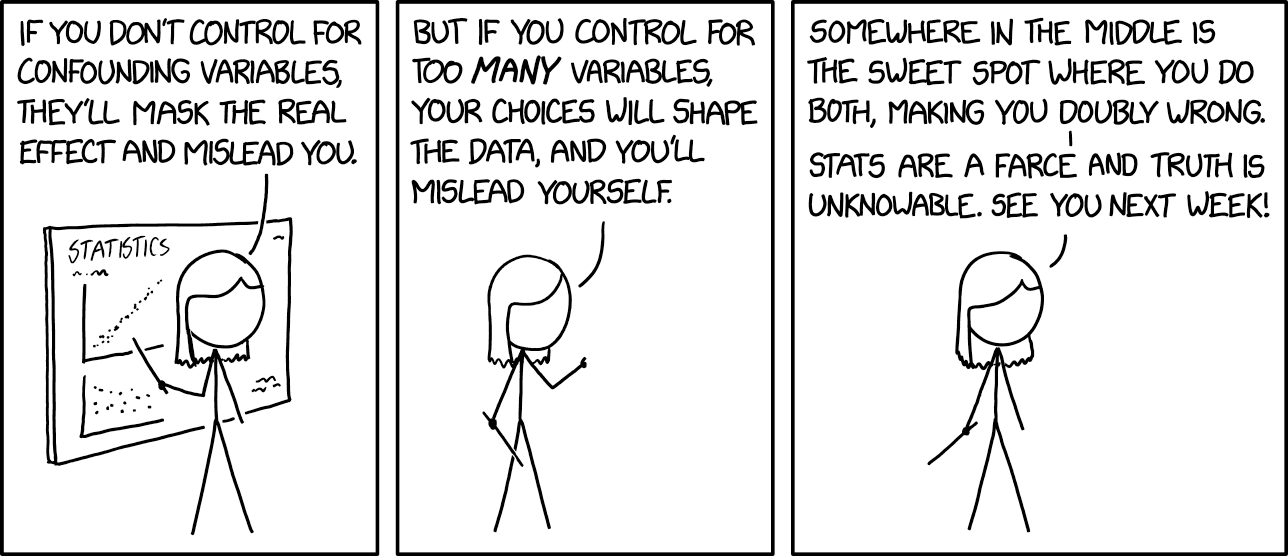
\includegraphics{images/confounding_variables.png}
\end{center}

\setlength{\abovedisplayskip}{-5pt}
\setlength{\abovedisplayshortskip}{-5pt}

{
\hypersetup{linkcolor=}
\setcounter{tocdepth}{2}
\tableofcontents
}
\listoffigures
\listoftables
\hypertarget{prefazione}{%
\chapter*{Prefazione}\label{prefazione}}


\emph{Data Science per psicologi} contiene il materiale delle lezioni dell'insegnamento di \emph{Psicometria B000286} (A.A. 2021/2022) rivolto agli studenti del primo anno del Corso di Laurea in Scienze e Tecniche Psicologiche dell'Università degli Studi di Firenze. \emph{Psicometria} si propone di fornire agli studenti un'introduzione all'analisi dei dati in psicologia. Le conoscenze/competenze che verranno sviluppate in questo insegnamento sono quelle della Data science, ovvero un insieme di conoscenze/competenze che si pongono all'intersezione tra statistica (ovvero, richiedono la capacità di comprendere teoremi statistici) e informatica (ovvero, richiedono la capacità di sapere utilizzare un software).

\hypertarget{la-psicologia-e-la-data-science}{%
\section*{La psicologia e la Data science}\label{la-psicologia-e-la-data-science}}


Sembra sensato spendere due parole su un tema che è importante per gli studenti: quello indicato dal titolo di questo Capitolo. È ovvio che agli studenti di psicologia la statistica non piace. Se piacesse, forse studierebbero Data science e non psicologia; ma non lo fanno. Di conseguenza, gli studenti di psicologia si chiedono: ``perché dobbiamo perdere tanto tempo a studiare queste cose quando in realtà quello che ci interessa è tutt'altro?'' Questa è una bella domanda.

C'è una ragione molto semplice che dovrebbe farci capire perché la Data science è così importante per la psicologia. Infatti, a ben pensarci, la psicologia è una disciplina intrinsecamente statistica, se per statistica intendiamo quella disciplina che studia la variazione delle caratteristiche degli individui nella popolazione. La psicologia studia \emph{gli individui} ed è proprio la variabilità inter- e intra-individuale ciò che vogliamo descrivere e, in certi casi, predire. In questo senso, la psicologia è molto diversa dall'ingegneria, per esempio. Le proprietà di un determinato ponte sotto certe condizioni, ad esempio, sono molto simili a quelle di un altro ponte, sotto le medesime condizioni. Quindi, per un ingegnere la statistica è poco importante: le proprietà dei materiali sono unicamente dipendenti dalla loro composizione e restano costanti. Ma lo stesso non può dirsi degli individui: ogni individuo è unico e cambia nel tempo. E le variazioni tra gli individui, e di un individuo nel tempo, sono l'oggetto di studio proprio della psicologia: è dunque chiaro che i problemi che la psicologia si pone sono molto diversi da quelli affrontati, per esempio, dagli ingegneri. Questa è la ragione per cui abbiamo tanto bisogno della Data science in psicologia: perché la Data science ci consente di descrivere la variazione e il cambiamento. E queste sono appunto le caratteristiche di base dei fenomeni psicologici.

Sono sicuro che, leggendo queste righe, a molti studenti sarà venuta in mente la seguente domanda: perché non chiediamo a qualche esperto di fare il ``lavoro sporco'' (ovvero le analisi statistiche) per noi, mentre noi (gli psicologi) ci occupiamo solo di ciò che ci interessa, ovvero dei problemi psicologici slegati dai dettagli ``tecnici'' della Data science? La risposta a questa domanda è che non è possibile progettare uno studio psicologico sensato senza avere almeno una comprensione rudimentale della Data science. Le tematiche della Data science non possono essere ignorate né dai ricercatori in psicologia né da coloro che svolgono la professione di psicologo al di fuori dell'Università. Infatti, anche i professionisti al di fuori dall'università non possono fare a meno di leggere la letteratura psicologica più recente: il continuo aggiornamento delle conoscenze è infatti richiesto dalla deontologia della professione. Ma per potere fare questo è necessario conoscere un bel po' di Data science! Basta aprire a caso una rivista specialistica di psicologia per rendersi conto di quanto ciò sia vero: gli articoli che riportano i risultati delle ricerche psicologiche sono zeppi di analisi statistiche e di modelli formali. E la comprensione della letteratura psicologica rappresenta un requisito minimo nel bagaglio professionale dello psicologo.

Le considerazioni precedenti cercano di chiarire il seguente punto: la Data science non è qualcosa da studiare a malincuore, in un singolo insegnamento universitario, per poi poterla tranquillamente dimenticare. Nel bene e nel male, gli psicologi usano gli strumenti della Data science in tantissimi ambiti della loro attività professionale: in particolare quando costruiscono, somministrano e interpretano i test psicometrici. È dunque chiaro che possedere delle solide basi di Data science è un tassello imprescindibile del bagaglio professionale dello psicologo. In questo insegnamento verrano trattati i temi base della Data science e verrà adottato un punto di vista bayesiano, che corrisponde all'approccio più recente e sempre più diffuso in psicologia.

\hypertarget{come-studiare}{%
\section*{Come studiare}\label{come-studiare}}


Il giusto metodo di studio per prepararsi all'esame di Psicometria è quello di seguire attivamente le lezioni, assimilare i concetti via via che essi vengono presentati e verificare in autonomia le procedure presentate a lezione. Incoraggio gli studenti a farmi domande per chiarire ciò che non è stato capito appieno. Incoraggio gli studenti a utilizzare i forum attivi su Moodle e, soprattutto, a svolgere gli esercizi proposti su Moodle. I problemi forniti su Moodle rappresentano il livello di difficoltà richiesto per superare l'esame e consentono allo studente di comprendere se le competenze sviluppate fino a quel punto sono sufficienti rispetto alle richieste dell'esame.

La prima fase dello studio, che è sicuramente individuale, è quella in cui è necessario acquisire le conoscenze teoriche relative ai problemi che saranno presentati all'esame. La seconda fase di studio, che può essere facilitata da scambi con altri e da incontri di gruppo, porta ad acquisire la capacità di applicare le conoscenze: è necessario capire come usare un software (\(\textsf{R}\)) per applicare i concetti statistici alla specifica situazione del problema che si vuole risolvere. Le due fasi non sono però separate: il saper fare molto spesso ci aiuta a capire meglio.

\hypertarget{sviluppare-un-metodo-di-studio-efficace}{%
\section*{Sviluppare un metodo di studio efficace}\label{sviluppare-un-metodo-di-studio-efficace}}


Avendo insegnato molte volte in passato un corso introduttivo di analisi dei dati ho notato nel corso degli anni che gli studenti con l'atteggiamento mentale che descriverò qui sotto generalmente ottengono ottimi risultati. Alcuni studenti sviluppano naturalmente questo approccio allo studio, ma altri hanno bisogno di fare uno sforzo per maturarlo. Fornisco qui sotto una breve descrizione del ``metodo di studio'' che, nella mia esperienza, è il più efficace per affrontare le richieste di questo insegnamento.

\begin{itemize}
\tightlist
\item
  Dedicate un tempo sufficiente al materiale di base, apparentemente facile; assicuratevi di averlo capito bene. Cercate le lacune nella vostra comprensione. Leggere presentazioni diverse dello stesso materiale (in libri o articoli diversi) può fornire nuove intuizioni.
\item
  Gli errori che facciamo sono i nostri migliori maestri. Istintivamente cerchiamo di dimenticare subito i nostri errori. Ma il miglior modo di imparare è apprendere dagli errori che commettiamo. In questo senso, una soluzione corretta è meno utile di una soluzione sbagliata. Quando commettiamo un errore questo ci fornisce un'informazione importante: ci fa capire qual è il materiale di studio sul quale dobbiamo ritornare e che dobbiamo capire meglio.
\item
  C'è ovviamente un aspetto ``psicologico'' nello studio. Quando un esercizio o problema ci sembra incomprensibile, la cosa migliore da fare è dire: ``mi arrendo'', ``non ho idea di cosa fare!''. Questo ci rilassa: ci siamo già arresi, quindi non abbiamo niente da perdere, non dobbiamo più preoccuparci. Ma non dobbiamo fermarci qui. Le cose ``migliori'' che faccio (se ci sono) le faccio quando non ho voglia di lavorare. Alle volte, quando c'è qualcosa che non so fare e non ho idea di come affontare, mi dico: ``oggi non ho proprio voglia di fare fatica'', non ho voglia di mettermi nello stato mentale per cui ``in 10 minuti devo risolvere il problema perché dopo devo fare altre cose''. Però ho voglia di \emph{divertirmi} con quel problema e allora mi dedico a qualche aspetto ``marginale'' del problema, che so come affrontare, oppure considero l'aspetto più difficile del problema, quello che non so come risolvere, ma invece di cercare di risolverlo, guardo come altre persone hanno affrontato problemi simili, opppure lo stesso problema in un altro contesto. Non mi pongo l'obiettivo ``risolvi il problema in 10 minuti'', ma invece quello di farmi un'idea ``generale'' del problema, o quello di capire un caso più specifico e più semplice del problema. Senza nessuna pressione. Infatti, in quel momento ho deciso di non lavorare (ovvero, di non fare fatica). Va benissimo se ``parto per la tangente'', ovvero se mi metto a leggere del materiale che sembra avere poco a che fare con il problema centrale (le nostre intuizioni e la nostra curiosità solitamente ci indirizzano sulla strada giusta). Quando faccio così, molto spesso trovo la soluzione del problema che mi ero posto e, paradossalmente, la trovo in un tempo minore di quello che, in precedenza, avevo dedicato a ``lavorare'' al problema. Allora perché non faccio sempre così? C'è ovviamente l'aspetto dei ``10 minuti'' che non è sempre facile da dimenticare. Sotto pressione, possiamo solo agire in maniera automatica, ovvero possiamo solo applicare qualcosa che già sappiamo fare. Ma se dobbiamo imparare qualcosa di nuovo, la pressione è un impedimento.
\item
  È utile farsi da soli delle domande sugli argomenti trattati, senza limitarsi a cercare di risolvere gli esercizi che vengono assegnati. Quando studio qualcosa mi viene in mente: ``se questo è vero, allora deve succedere quest'altra cosa''. Allora verifico se questo è vero, di solito con una simulazione. Se i risultati della simulazione sono quelli che mi aspetto, allora vuol dire che ho capito. Se i risultati sono diversi da quelli che mi aspettavo, allora mi rendo conto di non avere capito e ritorno indietro a studiare con più attenzione la teoria che pensavo di avere capito -- e ovviamente mi rendo conto che c'era un aspetto che avevo frainteso. Questo tipo di verifica è qualcosa che dobbiamo fare da soli, in prima persona: nessun altro può fare questo al posto nostro.
\item
  Non aspettatevi di capire tutto la prima volta che incontrate un argomento nuovo.\footnote{Ricordatevi inoltre che gli individui tendono a sottostimare la propria capacità di apprendere \citep{horn2021underestimating}.} È utile farsi una nota mentalmente delle lacune nella vostra comprensione e tornare su di esse in seguito per carcare di colmarle. L'atteggiamento naturale, quando non capiamo i dettagli di qualcosa, è quello di pensare: ``non importa, ho capito in maniera approssimativa questo punto, non devo preoccuparmi del resto''. Ma in realtà non è vero: se la nostra comprensione è superficiale, quando il problema verrà presentato in una nuova forma, non riusciremo a risolverlo. Per cui i dubbi che ci vengono quando studiamo qualcosa sono il nostro alleato più prezioso: ci dicono esattamente quali sono gli aspetti che dobbiamo approfondire per potere migliorare la nostra preparazione.
\item
  È utile sviluppare una visione d'insieme degli argomenti trattati, capire l'obiettivo generale che si vuole raggiungere e avere chiaro il contributo che i vari pezzi di informazione forniscono al raggiungimento di tale obiettivo. Questa organizzazione mentale del materiale di studio facilita la comprensione. È estremamente utile creare degli schemi di ciò che si sta studiando. Non aspettate che sia io a fornirvi un riepilogo di ciò che dovete imparare: sviluppate da soli tali schemi e tali riassunti.
\item
  Tutti noi dobbiamo imparare l'arte di trovare le informazioni, non solo nel caso di questo insegnamento. Quando vi trovate di fronte a qualcosa che non capite, o ottenete un oscuro messaggio di errore da un software, ricordatevi: ``Google is your friend''!
\end{itemize}

\begin{flushright}
Corrado Caudek\\
Marzo 2022 \end{flushright}

\mainmatter

\hypertarget{part-inferenza-bayesiana}{%
\part{Inferenza bayesiana}\label{part-inferenza-bayesiana}}

\hypertarget{ch:intro-bayes-inference}{%
\chapter{Flusso di lavoro bayesiano}\label{ch:intro-bayes-inference}}

La moderna statistica bayesiana viene per lo più eseguita utilizzando un linguaggio di programmazione probabilistico implementato su computer. Ciò ha cambiato radicalmente il modo in cui venivano eseguite le statistiche bayesiane anche fin pochi decenni fa. La complessità dei modelli che possiamo costruire è aumentata e la barriera delle competenze matematiche e computazionali che sono richieste è diminuita. Inoltre, il processo di modellazione iterativa è diventato, sotto molti aspetti, molto più facile da eseguire. Anche se formulare modelli statistici complessi è diventato più facile che mai, la statistica è un campo pieno di sottigliezze che non scompaiono magicamente utilizzando potenti metodi computazionali. Pertanto, avere una buona preparazione sugli aspetti teorici, specialmente quelli rilevanti nella pratica, è estremamente utile per applicare efficacemente i metodi statistici.

\hypertarget{modellizzazione-bayesiana}{%
\section{Modellizzazione bayesiana}\label{modellizzazione-bayesiana}}

L'analisi bayesiana corrisponde alla costruzione di un modello statistico che si può rappresentare con una quaterna

\begin{equation}
(\mathcal{Y}, p(y \mid \theta), p(\theta), \theta \in \Theta),
\end{equation}

dove \(\mathcal{Y}\) è l'insieme di tutti i possibili risultati ottenuti dall'esperimento casuale e \(p(y \mid \theta)\) è una famiglia di leggi di probabilità, indicizzata dal parametro \(\theta \in \Theta\), che descrive l'incertezza sull'esito dell'esperimento. Secondo l'approccio bayesiano, il parametro incognito \(\theta\) è considerato una variabile casuale che segue la legge di probabilità \(p(\theta)\). L'incertezza su \(\theta\) è la sintesi delle opinioni e delle informazioni che si hanno sul parametro prima di avere osservato il risultato dell'esperimento e prende il nome di \emph{distribuzione a priori}. La costruzione del modello statistico passa attraverso la scelta di una densità \(p(y \mid \theta)\) che rappresenta, in senso probabilistico, il fenomeno d'interesse, e attraverso la scelta di una distribuzione a priori \(p(\theta)\). Le informazioni che si hanno a priori sul parametro di interesse \(\theta\), contenute in \(p(\theta)\), vengono aggiornate attraverso quelle provenienti dal campione osservato \(y = (y_1, \dots, y_n)\) contenute nella funzione \(p(y \mid \theta)\), che, osservata come funzione di \(\theta\) per \(y\), prende il nome di \emph{funzione di verosimiglianza}. L'aggiornamento delle informazioni avviene attraverso la formula di Bayes

\begin{equation}
p(\theta \mid y) = \frac{p(y \mid \theta) p(\theta)}{\int_{\Theta}p(y \mid \theta) p(\theta) \,\operatorname {d}\!\theta} \quad \theta \in \Theta,
 \label{eq:bayes-intro}
\end{equation}

in cui \(p(\theta \mid y)\) prende il nome di \emph{distribuzione a posteriori}.

Il denominatore del Teorema di Bayes \eqref{eq:bayes-intro}, che costituisce la costante di normalizzazione, è la densità marginale dei dati (o verosimiglianza marginale). In ambito bayesiano la distribuzione a posteriori viene utilizzata per calcolare le principali quantità di interesse dell'inferenza, ad esempio la media a posteriori di \(\theta\).

Possiamo descrivere la modellazione bayesiana distinguendo tre passaggi \citep{martin2022bayesian}.

\begin{enumerate}
\def\labelenumi{\arabic{enumi}.}
\tightlist
\item
  Dati alcuni dati e alcune ipotesi su come questi dati potrebbero essere stati generati, progettiamo un modello combinando e trasformando variabili casuali.
\item
  Usiamo il teorema di Bayes per condizionare i nostri modelli ai dati disponibili. Chiamiamo questo processo ``inferenza'' e come risultato otteniamo una distribuzione a posteriori.
\item
  Critichiamo il modello verificando se il modello abbia senso utilizzando criteri diversi, inclusi i dati e la nostra conoscenza del dominio. Poiché generalmente siamo incerti sui modelli, a volte confrontiamo modelli diversi.
\end{enumerate}

Questi tre passaggi vengono eseguiti in modo iterativo e danno luogo a quello che è chiamato ``flusso di lavoro bayesiano'' (\emph{bayesian workflow}).

\hypertarget{notazione}{%
\subsection{Notazione}\label{notazione}}

Per fissare la notazione, nel seguito \(y\) rappresenterà i dati e \(\theta\) rappresenterà i parametri incogniti di un modello statistico. Sia \(y\) che \(\theta\) vengono concepiti come variabili casuali. Con \(x\) vengono invece denotate le quantità note, come ad esempio i predittori del modello lineare. Per rappresentare in un modo conciso i modelli probabilistici viene usata una notazione particolare. Ad esempio, invece di scrivere \(p(\theta) = \mbox{Beta}(1, 1)\) scriviamo \(\theta \sim \mbox{Beta}(1, 1)\). Il simbolo ``\(\sim\)'' viene spesso letto ``è distribuito come''. Possiamo anche pensare che significhi che \(\theta\) costituisce un campione casuale estratto dalla distribuzione Beta(1, 1). Allo stesso modo, ad esempio, la verosimiglianza del modello binomiale può essere scritta come \(y \sim \text{Bin}(n, \theta)\).

\hypertarget{distribuzioni-a-priori}{%
\section{Distribuzioni a priori}\label{distribuzioni-a-priori}}

Quando adottiamo un approccio bayesiano, i parametri della distribuzione di riferimento non venono considerati come delle costanti incognite ma bensì vengono trattati come variabili casuali; di conseguenza, i parametri assumono una particolare distribuzione che nelle statistica bayesiana viene definita ``a priori''. I parametri (o il parametro), che possiamo indicare con \(\theta\), possono assumere delle distribuzioni a priori differenti: a seconda delle informazioni disponibili bisogna selezionare una distribuzione di \(\theta\) in modo tale che venga assegnata una probabilità maggiore a quei valori che si ritengono più plausibili per \(\theta\). Idealmente, le credenze a priori che portano alla specificazione di una distribuzione a priori dovrebbero essere supportate da una qualche motivazione, come ad esempio i risultati di ricerche precedenti.

\hypertarget{tipologie-di-distribuzioni-a-priori}{%
\subsection{Tipologie di distribuzioni a priori}\label{tipologie-di-distribuzioni-a-priori}}

Possiamo distinguere tra diverse distribuzioni a priori in base a quanto fortemente impegnano il ricercatore a ritenere come plausibile un particolare intervallo di valori dei parametri. Il caso più estremo è quello che rivela una totale assenza di conoscenze a priori, il che conduce alle \emph{distribuzioni a priori non informative}, ovvero quelle che assegnano lo stesso livello di credibilità a tutti i valori dei parametri. Le distribuzioni a priori informative, d'altra parte, possono essere \emph{debolmente informative} o \emph{fortemente informative}, a seconda della forza della credenza che esprimono. Il caso più estremo di credenza a priori è quello che riassume il punto di vista del ricercatore nei termini di un \emph{unico valore} del parametro, il che assegna tutta la probabilità (massa o densità) ad di un singolo valore del parametro. Poiché questa non è più una distribuzione di probabilità, sebbene ne soddisfi la definizione, in questo caso si parla di una \emph{distribuzione a priori degenerata}. La figura seguente motra alcuni esempi di distribuzioni a priori per il modello Binomiale:

\begin{itemize}
\tightlist
\item
  distribuzione \emph{non informativa}: \(\theta_c \sim \mbox{Beta}(1,1)\);
\item
  distribuzione \emph{debolmente informativa}: \(\theta_c \sim \mbox{Beta}(5,2)\);
\item
  distribuzione \emph{fortemente informativa}: \(\theta_c \sim \mbox{Beta}(50,20)\);
\item
  \emph{valore puntuale}: \(\theta_c \sim \mbox{Beta}(\alpha, \beta)\) con \(\alpha, \beta \rightarrow \infty\) e \(\frac{\alpha}{\beta} = \frac{5}{2}\).
\end{itemize}

\begin{figure}[h]

{\centering 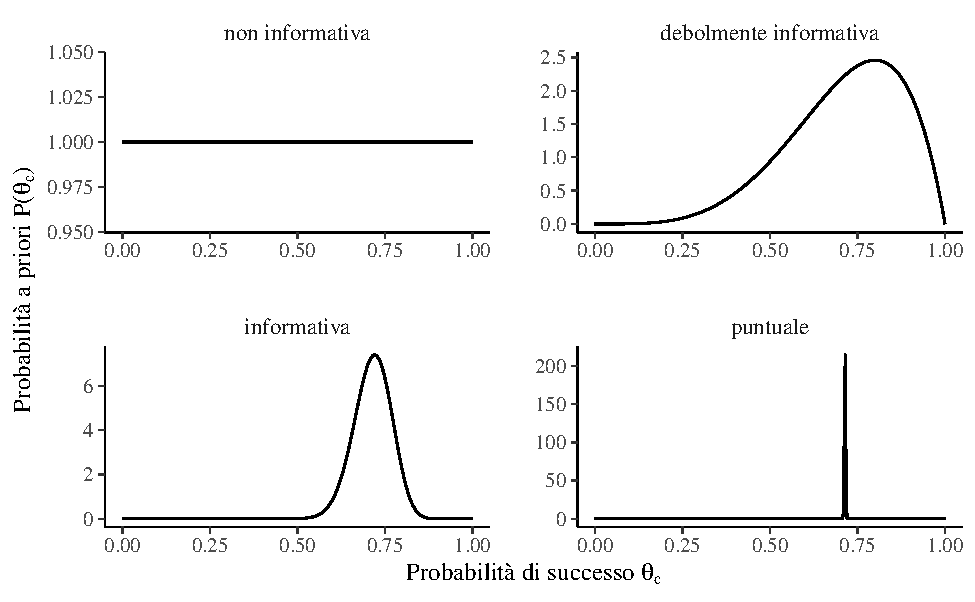
\includegraphics{ds4psy_files/figure-latex/unnamed-chunk-3-1} 

}

\caption{Esempi di distribuzioni a priori per il parametro $\theta_c$ nel Modello Binomiale.}\label{fig:unnamed-chunk-3}
\end{figure}

\hypertarget{selezione-della-distribuzione-a-priori}{%
\subsection{Selezione della distribuzione a priori}\label{selezione-della-distribuzione-a-priori}}

La selezione delle distribuzioni a priori è stata spesso vista come una delle scelte più importanti che un ricercatore fa quando implementa un modello bayesiano in quanto può avere un impatto sostanziale sui risultati finali. La soggettività delle distribuzioni a priori è evidenziata dai critici come un potenziale svantaggio dei metodi bayesiani. A questa critica, \citet{vandeSchoot2021modelling} rispondono dicendo che, al di là della scelta delle distribuzioni a priori, ci sono molti elementi del processo di inferenza statistica che sono soggettivi, ovvero la scelta del modello statistico e le ipotesi sulla distribuzione degli errori. In secondo luogo, \citet{vandeSchoot2021modelling} notano come le distribuzioni a priori svolgono due importanti ruoli statistici: quello della ``regolarizzazione della stima'', ovvero, il processo che porta ad indebolire l'influenza indebita di osservazioni estreme, e quello del miglioramento dell'efficienza della stima, ovvero, la facilitazione dei processi di calcolo numerico di stima della distribuzione a posteriori. L'effetto della distribuzione a priori sulla distribuzione a posteriori verrà discusso in dettaglio nel Capitolo \ref{chapter-balance}.

\hypertarget{un-esempio-concreto}{%
\subsection{Un esempio concreto}\label{un-esempio-concreto}}

Per introdurre la modelizzazione bayesiana useremo qui i dati riportati da \citet{zetschefuture2019} (si veda l'appendice \ref{appendix:future-exp}). Tali dati corrispondono a 23 ``successi'' in 30 prove e possono dunque essere considerati la manifestazione di una variabile casuale Bernoulliana.

Se non abbiamo alcuna informazione a priori su \(\theta\) (ovvero, la probabilità che l'aspettativa dell'umore futuro del partecipante sia distorta negativamente), potremmo pensare di usare una distribuzione a priori uniforme, ovvero una Beta di parametri \(\alpha=1\) e \(\beta=1\). Una tale scelta, tuttavia, è sconsigliata in quanto è più vantaggioso usare una distribuzione debolmente informativa, come ad esempio \(\mbox{Beta}(2, 2)\), che ha come scopo la regolarizzazione, cioè quello di mantenere le inferenze in un intervallo ragionevole. Qui useremo una \(\mbox{Beta}(2, 10)\).

\[
p(\theta) = \frac{\Gamma(12)}{\Gamma(2)\Gamma(10)}\theta^{2-1} (1-\theta)^{10-1}.
\]

\begin{Shaded}
\begin{Highlighting}[]
\NormalTok{bayesrules}\SpecialCharTok{::}\FunctionTok{plot\_beta}\NormalTok{(}\AttributeTok{alpha =} \DecValTok{2}\NormalTok{, }\AttributeTok{beta =} \DecValTok{10}\NormalTok{, }\AttributeTok{mean =} \ConstantTok{TRUE}\NormalTok{, }\AttributeTok{mode =} \ConstantTok{TRUE}\NormalTok{)}
\end{Highlighting}
\end{Shaded}

\begin{center}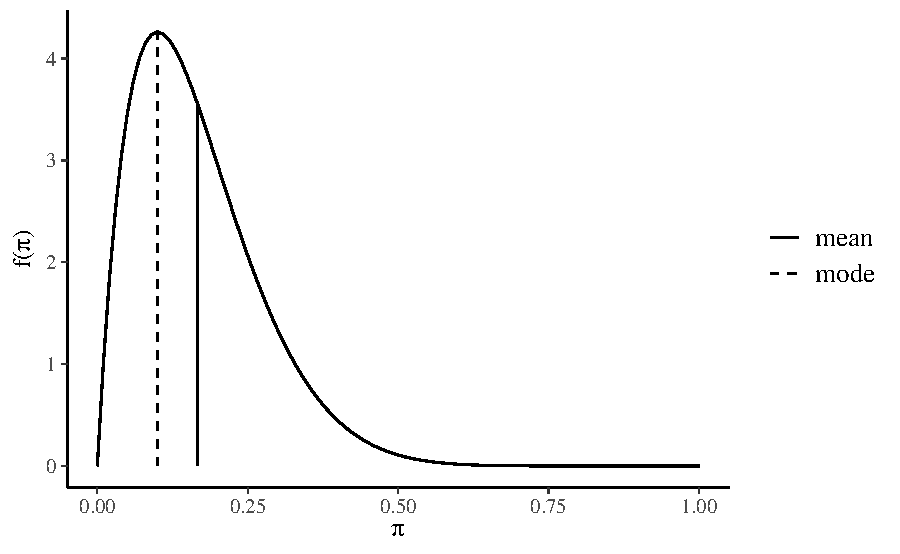
\includegraphics{ds4psy_files/figure-latex/unnamed-chunk-4-1} \end{center}

La \(\mbox{Beta}(2, 10)\) esprime la credenza che \(\theta\) assume valori \(< 0.5\), con il valore più plausibile pari a circa 0.1. Questo è assolutamente implausibile per il caso dell'esempio in discussione: la \(\mbox{Beta}(2, 10)\) verrà usata solo per scopi didattici, ovvero, per esplorare le conseguenze di tale scelta sulla distribuzione a posteriori.

\hypertarget{la-funzione-di-verosimiglianza}{%
\section{La funzione di verosimiglianza}\label{la-funzione-di-verosimiglianza}}

Iniziamo con una definizione.

\begin{definition}
La \emph{funzione di verosimiglianza} \(\mathcal{L}(\theta \mid y) = f(y \mid \theta), \theta \in \Theta,\) è la funzione di massa o di densità di probabilità dei dati \(y\) vista come una funzione del parametro sconosciuto (o dei parametri sconosciuti) \(\theta\).
\end{definition}

Detto in altre parole, le funzioni di verosimiglianza e di (massa o densità di) probabilità sono formalmente identiche, ma è completamente diversa la loro interpretazione. Nel caso della funzione di massa o di densità di probabilità la distribuzione del vettore casuale delle osservazioni campionarie \(y\) dipende dai valori assunti dal parametro (o dai parametri) \(\theta\); nel caso della la funzione di verosimiglianza la credibilità assegnata a ciascun possibile valore \(\theta\) viene determinata avendo acquisita l'informazione campionaria \(y\) che rappresenta l'elemento condizionante. In altri termini, la funzione di verosimiglianza descrive in termini relativi il sostegno empirico che \(\theta \in \Theta\) riceve da \(y\). Infatti, la funzione di verosimiglianza assume forme diverse al variare di \(y\). Possiamo dunque pensare alla funzione di verosimiglianza come alla risposta alla seguente domanda: avendo osservato i dati \(y\), quanto risultano (relativamente) credibili i diversi valori del parametro \(\theta\)? In termini più formali possiamo dire: sulla base dei dati, \(\theta_1 \in \Theta\) risulta più credibile di \(\theta_2 \in \Theta\) quale indice del modello probabilistico generatore dei dati se \(\mathcal{L}(\theta_1) > \mathcal{L}(\theta_1)\).

Notiamo un punto importante: la funzione \(\mathcal{L}(\theta \mid y)\) non è una funzione di densità. Infatti, essa non racchiude un'area unitaria.

\hypertarget{notazione-1}{%
\subsection{Notazione}\label{notazione-1}}

Seguendo una pratica comune, in questa dispensa spesso useremo la notazione \(p(\cdot)\) per rappresentare due quantità differenti, ovvero la funzione di verosimiglianza e la distribuzione a priori. Questo piccolo abuso di notazione riflette il seguente punto di vista: anche se la verosimiglianza non è una funzione di densità di probabilità, noi non vogliamo stressare questo aspetto, ma vogliamo piuttosto pensare alla verosimiglianza e alla distribuzione a priori come a due elementi che sono egualmente necessari per calcolare la distribuzione a posteriori. In altri termini, per così dire, questa notazione assegna lo stesso status epistemologico alle due diverse quantità che si trovano al numeratore della regola di Bayes.

\hypertarget{la-log-verosimiglianza}{%
\subsection{La log-verosimiglianza}\label{la-log-verosimiglianza}}

Dal punto di vista pratico risulta più conveniente utilizzare, al posto della funzione di verosimiglianza, il suo logaritmo naturale, ovvero la funzione di log-verosimiglianza:

\begin{equation}
\ell(\theta) = \log \mathcal{L}(\theta).
\end{equation}

Poiché il logaritmo è una funzione strettamente crescente (usualmente si considera il logaritmo naturale), allora \(\mathcal{L}(\theta)\) e \(\ell(\theta)\) assumono il massimo (o i punti di massimo) in corrispondenza degli stessi valori di \(\theta\) (per un approfondimento, si veda l'Appendice \ref{appendix:max-like}):

\[
\hat{\theta} = \argmax_{\theta \in \Theta} \ell(\theta) = \argmax_{\theta \in \Theta} \mathcal{L}(\theta).
\]

Per le proprietà del logaritmo, si ha

\begin{equation}
\ell(\theta) = \log \left( \prod_{i = 1}^n f(y \mid \theta) \right) = \sum_{i = 1}^n \log f(y \mid \theta).
\end{equation}

Si noti che non è necessario lavorare con i logaritmi, ma è fortemente consigliato. Il motivo è che i valori della verosimiglianza, in cui si moltiplicano valori di probabilità molto piccoli, possono diventare estremamente piccoli -- qualcosa come \(10^{-34}\). In tali circostanze, non è sorprendente che i programmi dei computer mostrino problemi di arrotondamento numerico. Le trasformazioni logaritmiche risolvono questo problema.

\hypertarget{un-esempio-concreto-1}{%
\subsection{Un esempio concreto}\label{un-esempio-concreto-1}}

Se i dati di \citet{zetschefuture2019} possono essere riassunti da una proporzione allora è sensato adottare un modello probabilistico binomiale quale meccanismo generatore dei dati:

\begin{equation}
y  \sim \mbox{Bin}(n, \theta),
\label{eq:binomialmodel}
\end{equation}

laddove \(\theta\) è la probabiltà che una prova Bernoulliana assuma il valore 1 e \(n\) corrisponde al numero di prove Bernoulliane. Questo modello assume che le prove Bernoulliane \(y_i\) che costituiscono il campione \(y\) siano tra loro indipendenti e che ciascuna abbia la stessa probabilità \(\theta \in [0, 1]\) di essere un ``successo'' (valore 1). In altre parole, il modello generatore dei dati avrà una funzione di massa di probabilità

\[
p(y \mid \theta)
\ = \
\mbox{Bin}(y \mid n, \theta).
\]

Nei capitoli precedenti è stato mostrato come, sulla base del modello binomiale, sia possibile assegnare una probabilità a ciascun possibile valore \(y \in \{0, 1, \dots, n\}\) \emph{assumendo noto il valore del parametro} \(\theta\). Ma ora abbiamo il problema inverso, ovvero quello di fare inferenza su \(\theta\) alla luce dei dati campionari \(y\). In altre parole, riteniamo di conoscere il modello probabilistico che ha generato i dati, ma di tale modello non conosciamo i parametri: vogliamo dunque ottenere informazioni su \(\theta\) avendo osservato i dati \(y\).

Per i dati di \citet{zetschefuture2019} la funzione di verosimiglianza corrisponde alla funzione binomiale di parametro \(\theta \in [0, 1]\) sconosciuto. Abbiamo osservato un ``successo'' 23 volte in 30 ``prove'', dunque, \(y = 23\) e \(n = 30\). La funzione di verosimiglianza diventa

\begin{equation}
\mathcal{L}(\theta \mid y) = \frac{(23 + 7)!}{23!7!} \theta^{23} + (1-\theta)^7.
\label{eq:likebino23}
\end{equation}

Per costruire la funzione di verosimiglianza dobbiamo applicare la \eqref{eq:likebino23} tante volte, cambiando ogni volta il valore \(\theta\) ma \emph{tenendo sempre costante il valore dei dati}. Per esempio, se poniamo \(\theta = 0.1\)

\[
\mathcal{L}(\theta \mid y) = \frac{(23 + 7)!}{23!7!} 0.1^{23} + (1-0.1)^7
\]

otteniamo

\begin{Shaded}
\begin{Highlighting}[]
\FunctionTok{dbinom}\NormalTok{(}\DecValTok{23}\NormalTok{, }\DecValTok{30}\NormalTok{, }\FloatTok{0.1}\NormalTok{)}
\CommentTok{\#\textgreater{} [1] 9.737e{-}18}
\end{Highlighting}
\end{Shaded}

Se poniamo \(\theta = 0.2\)

\[
\mathcal{L}(\theta \mid y) = \frac{(23 + 7)!}{23!7!} 0.2^{23} + (1-0.2)^7
\]

otteniamo

\begin{Shaded}
\begin{Highlighting}[]
\FunctionTok{dbinom}\NormalTok{(}\DecValTok{23}\NormalTok{, }\DecValTok{30}\NormalTok{, }\FloatTok{0.2}\NormalTok{)}
\CommentTok{\#\textgreater{} [1] 3.581e{-}11}
\end{Highlighting}
\end{Shaded}

e così via. La figura \ref{fig:likefutexpect} --- costruita utilizzando 100 valori equispaziati \(\theta \in [0, 1]\) --- fornisce una rappresentazione grafica della funzione di verosimiglianza.

\begin{Shaded}
\begin{Highlighting}[]
\NormalTok{n }\OtherTok{\textless{}{-}} \DecValTok{30}
\NormalTok{y }\OtherTok{\textless{}{-}} \DecValTok{23}
\NormalTok{theta }\OtherTok{\textless{}{-}} \FunctionTok{seq}\NormalTok{(}\DecValTok{0}\NormalTok{, }\DecValTok{1}\NormalTok{, }\AttributeTok{length.out =} \DecValTok{100}\NormalTok{)}
\NormalTok{like }\OtherTok{\textless{}{-}} \FunctionTok{choose}\NormalTok{(n, y) }\SpecialCharTok{*}\NormalTok{ theta}\SpecialCharTok{\^{}}\NormalTok{y }\SpecialCharTok{*}\NormalTok{ (}\DecValTok{1} \SpecialCharTok{{-}}\NormalTok{ theta)}\SpecialCharTok{\^{}}\NormalTok{(n }\SpecialCharTok{{-}}\NormalTok{ y)}
\FunctionTok{tibble}\NormalTok{(theta, like) }\SpecialCharTok{\%\textgreater{}\%}
  \FunctionTok{ggplot}\NormalTok{(}\FunctionTok{aes}\NormalTok{(}\AttributeTok{x =}\NormalTok{ theta, }\AttributeTok{y =}\NormalTok{ like)) }\SpecialCharTok{+}
  \FunctionTok{geom\_line}\NormalTok{() }\SpecialCharTok{+}
  \FunctionTok{labs}\NormalTok{(}
    \AttributeTok{y =} \FunctionTok{expression}\NormalTok{(}\FunctionTok{L}\NormalTok{(theta)),}
    \AttributeTok{x =} \FunctionTok{expression}\NormalTok{(}\StringTok{"Valori possibili di"} \SpecialCharTok{\textasciitilde{}}\NormalTok{ theta)}
\NormalTok{  )}
\end{Highlighting}
\end{Shaded}

\begin{figure}[h]

{\centering 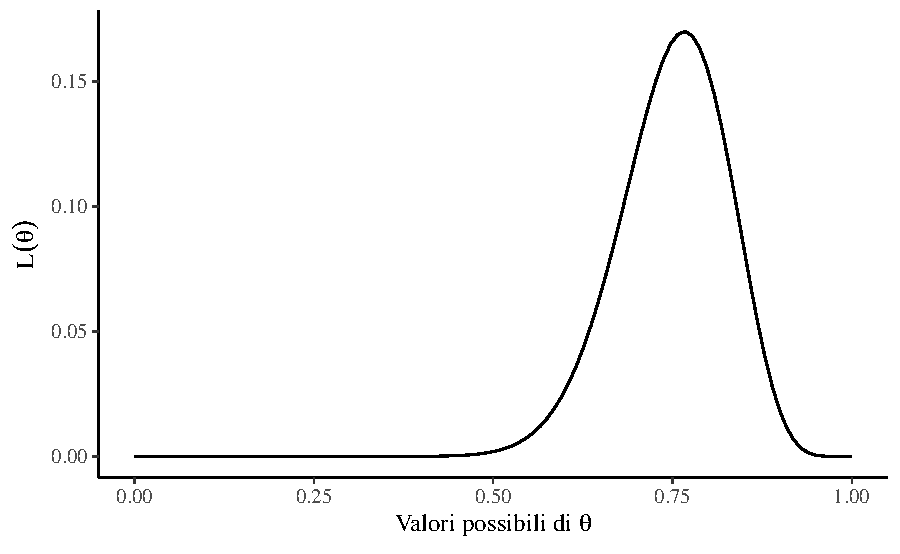
\includegraphics{ds4psy_files/figure-latex/likefutexpect-1} 

}

\caption{Funzione di verosimiglianza nel caso di 23 successi in 30 prove.}\label{fig:likefutexpect}
\end{figure}

Come possiamo interpretare la curva che abbiamo ottenuto? Per alcuni valori \(\theta\) la funzione di verosimiglianza assume valori piccoli; per altri valori \(\theta\) la funzione di verosimiglianza assume valori più grandi. Questi ultimi sono i valori di \(\theta\) più credibili e il valore 23/30 (la moda della funzione di verosimiglianza) è il valore più credibile di tutti.

\hypertarget{sec:const-normaliz-bino23}{%
\section{La verosimiglianza marginale}\label{sec:const-normaliz-bino23}}

Per il calcolo di \(p(\theta \mid y)\) è necessario dividere il prodotto tra la distribuzione a priori e la verosimiglianza per una costante di normalizzazione. Tale costante di normalizzazione, detta \emph{verosimiglianza marginale}, ha lo scopo di fare in modo che \(p(\theta \mid y)\) abbia area unitaria.

Si noti che, nel caso di variabili continue, la verosimiglianza marginale è espressa nei termini di un integrale. Tranne in pochi casi particolari, tale integrale non ha una soluzione analitica. Per questa ragione, l'inferenza bayesiana procede calcolando una approssimazione della distribuzione a posteriori mediante metodi numerici.

\hypertarget{un-esempio-concreto-2}{%
\subsection{Un esempio concreto}\label{un-esempio-concreto-2}}

Consideriamo nuovamente i dati di \citet{zetschefuture2019}. Supponiamo che nel numeratore bayesiano la verosimiglianza sia moltiplicata per una distribuzione uniforme, ovvero \(\mbox{Beta}(1, 1)\). In tali circostanze, il prodotto si riduce alla funzione di verosimiglianza. Per i dati di \citet{zetschefuture2019}, dunque, la costante di normalizzazione per si ottiene marginalizzando la funzione di verosimiglianza \(p(y = 23, n = 30 \mid \theta)\) sopra \(\theta\), ovvero risolvendo l'integrale:

\begin{equation}
p(y = 23, n = 30) = \int_0^1 \binom{30}{23} \theta^{23} (1-\theta)^{7} \,\operatorname {d}\!\theta.
\label{eq:intlikebino23}
\end{equation}

Una soluzione numerica si trova facilmente usando \(\R\):

\begin{Shaded}
\begin{Highlighting}[]
\NormalTok{like\_bin }\OtherTok{\textless{}{-}} \ControlFlowTok{function}\NormalTok{(theta) \{}
  \FunctionTok{choose}\NormalTok{(}\DecValTok{30}\NormalTok{, }\DecValTok{23}\NormalTok{) }\SpecialCharTok{*}\NormalTok{ theta}\SpecialCharTok{\^{}}\DecValTok{23} \SpecialCharTok{*}\NormalTok{ (}\DecValTok{1} \SpecialCharTok{{-}}\NormalTok{ theta)}\SpecialCharTok{\^{}}\DecValTok{7}
\NormalTok{\}}
\FunctionTok{integrate}\NormalTok{(like\_bin, }\AttributeTok{lower =} \DecValTok{0}\NormalTok{, }\AttributeTok{upper =} \DecValTok{1}\NormalTok{)}\SpecialCharTok{$}\NormalTok{value}
\CommentTok{\#\textgreater{} [1] 0.03226}
\end{Highlighting}
\end{Shaded}

La derivazione analitica è fornita nell'Appendice \ref{appendix:const-norm-bino23}.

\hypertarget{distribuzione-a-posteriori}{%
\section{Distribuzione a posteriori}\label{distribuzione-a-posteriori}}

La distribuzione a postreriori si trova applicando il teorema di Bayes:

\[
\text{probabilità a posteriori} = \frac{\text{probabilità a priori} \cdot \text{verosimiglianza}}{\text{costante di normalizzazione}}
\]

Una volta trovata la distribuzione a posteriori, possiamo usarla per derivare altre quantità di interesse. Questo viene generalmente ottenuto calcolando il valore atteso:

\[
J = \int f(\theta) p(\theta \mid y) \,\operatorname {d}\!y
\]

Se \(f(\cdot)\) è la funzione identità, ad esempio, \(J\) risulta essere la media di \(\theta\):

\[
\bar{\theta} = \int_{\Theta} \theta p(\theta \mid y) \,\operatorname {d}\!\theta .
\]

Ripeto qui quanto detto sopra: le quantità di interesse della statistica bayesiana(costante di normalizzazione, valore atteso della distribuzione a posteriori, ecc.) contengono integrali che risultano, nella maggior parte dei casi, impossibili da risolvere analiticamente. Per questo motivo, si ricorre a metodi di stima numerici, in particolare a quei metodi Monte Carlo basati sulle proprietà delle catene di Markov (MCMC). Questo argomento verrà discusso nel Capitolo \ref{ch:metropolis}.

\hypertarget{distribuzione-predittiva-a-priori}{%
\section{Distribuzione predittiva a priori}\label{distribuzione-predittiva-a-priori}}

La distribuzione a posteriori è l'oggetto centrale nella statistica bayesiana, ma non è l'unico. Oltre a fare inferenze sui valori dei parametri, potremmo voler fare inferenze sui dati. Questo può essere fatto calcolando la \emph{distribuzione predittiva a priori}:

\begin{equation}
p(y^*) = \int_\Theta p(y^* \mid \theta) p(\theta) \,\operatorname {d}\!\theta .
\label{eq:prior-pred-distr}
\end{equation}

La \eqref{eq:prior-pred-distr} descrive la distribuzione prevista dei dati in base al modello (che include la distribuzione a priori e la verosimiglianza), ovvero descrive i dati \(y^*\) che ci aspettiamo di osservare, dato il modello, prima di avere osservato i dati del campione.

È possibile utilizzare campioni dalla distribuzione predittiva a priori per valutare e calibrare i modelli utilizzando le nostre conoscenze dominio-specifiche. Ad esempio, ci possiamo chiedere: ``È sensato che un modello dell'altezza umana preveda che un essere umano sia alto -1.5 metri?''. Già prima di misurare una singola persona, possiamo renderci conto dell'assurdità di questa domanda. Se la distribuzione prevista dei dati consente domande di questo tipo (ovvero, prevede di osservare dati che risultano insensati alla luce delle nostre conoscenze dominio-specifiche), è chiaro che il modello deve essere riformulato.

\hypertarget{distribuzione-predittiva-a-posteriori}{%
\section{Distribuzione predittiva a posteriori}\label{distribuzione-predittiva-a-posteriori}}

Un'altra quantità utile da calcolare è la distribuzione predittiva a posteriori:

\begin{equation}
p(\tilde{y} \mid y) = \int_\Theta p(\tilde{y} \mid \theta) p(\theta \mid y) \,\operatorname {d}\!\theta .
\label{eq:post-pred-distr}
\end{equation}

Questa è la distribuzione dei dati attesi futuri \(\tilde{y}\) alla luce della distribuzione a posteriori \(p(\theta \mid y)\), che a sua volta è una conseguenza del modello adottato (distribuzione a priori e verosimiglianza) e dei dati osservati. In altre parole, questi sono i dati che il modello si aspetta dopo aver osservato i dati de campione. Dalla \eqref{eq:post-pred-distr} possiamo vedere che le previsioni sui dati attesi futuri sono calcolate integrando (o marginalizzando) sulla distribuzione a posteriori dei parametri. Di conseguenza, le previsioni calcolate in questo modo incorporano l'incertezza relativa alla stima dei parametri del modello.

\hypertarget{commenti-e-considerazioni-finali}{%
\section*{Commenti e considerazioni finali}\label{commenti-e-considerazioni-finali}}


Questo Capitolo ha brevemente passato in rassegna i concetti di base dell'inferenza statistica bayesiana. In base all'approccio bayesiano, invece di dire che il parametro di interesse di un modello statistico ha un valore vero ma sconosciuto, diciamo che, prima di eseguire l'esperimento, è possibile assegnare una distribuzione di probabilità, che chiamano stato di credenza, a quello che è il vero valore del parametro. Questa distribuzione a priori può essere nota (per esempio, sappiamo che la distribuzione dei punteggi del QI è normale con media 100 e deviazione standard 15) o può essere del tutto arbitraria. L'inferenza bayesiana procede poi nel modo seguente: si raccolgono alcuni dati e si calcola la probabilità dei possibili valori del parametro alla luce dei dati osservati e delle credenze a priori. Questa nuova distribuzione di probabilità è chiamata ``distribuzione a posteriori'' e riassume l'incertezza dell'inferenza.

\hypertarget{chapter-distr-coniugate}{%
\chapter{Distribuzioni a priori coniugate}\label{chapter-distr-coniugate}}

Obiettivo di questo Capitolo è fornire un esempio di derivazione della distribuzione a posteriori scegliendo quale distribuzione a priori una distribuzione coniugata. Esamineremo qui il modello Beta-Binomiale.

\hypertarget{pensare-a-una-proporzione-in-termini-soggettivi}{%
\section{Pensare a una proporzione ``in termini soggettivi''}\label{pensare-a-una-proporzione-in-termini-soggettivi}}

Nei problemi tradizionali di teoria delle probabilità ci sono molti esempi che riguardano l'estrazizone di palline colorate da un'urna. In questi esempi, ci viene fornito il numero di palline di vari colori nell'urna e ci viene chiesto di calcolare le probabilità di vari eventi. Ad esempio, in una scatola ci sono 40 palline bianche e 20 rosse. Se estrai due palline a caso, qual è la probabilità che entrambe siano bianche?

L'approccio bayesiano considera uno scenario diverso: quello in cui non conosciamo le proporzioni delle palline colorate nell'urna. Cioè, nell'esempio precedente, sappiamo solo che ci sono due tipi di palline colorate nell'urna, ma non sappiamo che 40 palline su 60 sono bianche (proporzione di bianco = \(2/3\)) e 20 delle 60 palline sono rosse (proporzione di rosso = \(1/3\)). Ci poniamo la seguente domanda: è possibile inferire le proporzioni cercate estraendo un campione di palline dall'urna e osservando i colori delle palline nel campione? Espresso in questo modo, questo diventa un problema di inferenza statistica, perché stiamo cercando di inferire la proporzione \(\pi\) della popolazione sulla base di un campione casuale della popolazione. Per continuare con l'esempio precedente, quello che ci chiediamo è: come è possibile inferire \(\pi\), la proporzione di palline rosse nella popolazione, in base al numero (per esempio, 10) di palline rosse e bianche che osserviamo nel campione?

Le proporzioni assomigliano alle probabilità. Ricordiamo che sono state proposte tre diverse interpretazioni del concetto di una probabilità.

\begin{itemize}
\tightlist
\item
  Il punto di vista classico: è necessario enumerare tutti gli eventi elementari dello spazio campionario in cui ogni risultato è ugualmente probabile.
\item
  Il punto di vista frequentista: è necessario ripetere l'esperimento esperimento casuale (cioè l'estrazione del campione) molte volte in condizioni identiche.
\item
  La visione soggettiva: è necessario esprimere la propria opinione sulla probabilità di un evento unico e irripetibile.
\end{itemize}

La visione classica non sembra potere funzionare qui, perché sappiamo solo che ci sono due tipi di palline colorate e il numero totale di palline è 60. Anche se estraiamo un campione di 10 palline, possiamo solo osservare la proporzione di palline rosse palline nel campione. Non c'è modo per stabilire quali sono le proprietà dello spazio campionario in cui ogni risultato è ugualmente probabile.

La visione frequentista potrebbe funzionare nel caso presente. Possiamo considerare il processo del campionamento (cioè l'estrazione di un campione casuale di 10 palline dall'urna) come un esperimento casuale che produce una proporzione campionaria \(p\). Potremmo quindi pensare di ripetere l'esperimento molte volte nelle stesse condizioni, ottenere molte proporzioni campionarie \(p\) e riassumere poi in qualche modo questa distribuzione di statistiche campionarie. Ripetendo l'esperimento casuale tante volte è possibile ottenere una stima abbastanza accurata della proporzione \(\pi\) di palline rosse nell'urna. Questo processo è fattibile, ma è però noioso, dispendioso in termini di tempo e soggetto a errori.

La visione soggettivista concepisce invece la probabilità sconosciuta \(\pi\) come un'opinione soggettiva di cui possiamo essere più o meno sicuri. Abbiamo visto in precedenza come questa opinione soggettiva dipende da due fonti di evidenza: le nostre credenze iniziali e le nuove informazioni fornite dai dati che abbiamo osservato. Vedremo in questo capitolo come sia possibile combinare le credenze iniziali rispetto al possibile valore \(\pi\) con le evidenza fornite dai dati per giungere ad una credenza a posteriori su \(\pi\). Se le nostre credenze a priori sono espresse nei termini di una distribuzione Beta, allora è possibile derivare le proprietà della distribuzione a priori per via analitica. Questo capitolo ha lo scopo di mostrare come questo possa essere fatto.

\hypertarget{il-denominatore-bayesiano}{%
\section{Il denominatore bayesiano}\label{il-denominatore-bayesiano}}

In termini generali possiamo dire che, in un problema bayesiano, i dati \(y\) provengono da una distribuzione \(p(y \mid \theta)\) e al parametro \(\theta\) viene assegnata una distribuzione a priori \(p(\theta)\). La scelta della distribuzione a priori ha importanti conseguenze di tipo computazionale. Infatti, a meno di non utilizzare particolari forme analitiche, risulta impossibile ottenere espressioni esplicite per la distribuzione a posteriori. Ciò dipende dall'espressione a denominatore della formula di Bayes

\begin{equation}
p(\theta \mid y) = \frac{p(\theta) p(y \mid \theta)}{\int p(\theta) p(y \mid \theta) \,\operatorname {d}\! \theta} \notag
\end{equation}

il cui calcolo, in generale, non è eseguibile in modo analitico in forma chiusa. Una soluzione analitica dell'integrale al denominatore della regola di Bayes è possibile solo se vengono usate distribuzioni provenienti da famiglie coniugate.

\begin{definition}
Una distribuzione di probabilità a priori \(p(\theta)\) si dice \emph{coniugata} al modello usato se la distribuzione a priori e la distribuzione a posteriori hanno la stessa forma funzionale. Dunque, le due distribuzioni differiscono solo per il valore dei parametri.
\end{definition}

\noindent Ad esempio, se la verosimiglianza è Poisson e la distribuzione a priori è Gamma, allora anche la distribuzione a posteriori sarà una distribuzione Gamma. Da un punto di vista puramente matematico, le distribuzioni a priori coniugate sono la scelta più conveniente in quanto ci consentono di calcolare analiticamente la distribuzione a posteriori con ``carta e penna'', senza la necessità di ricorrere a calcoli complessi. Da una prospettiva computazionale moderna, però, le distribuzioni a priori coniugate generalmente non sono migliori delle alternative, dato che i moderni metodi computazionali ci consentono di eseguire l'inferenza praticamente con qualsiasi scelta delle distribuzioni a priori, e non solo con quelle che sono matematicamente convenienti. Tuttavia, le famiglie coniugate offronto un utile ausilio didattico nello studio dell'inferenza bayesiana (e anche in alcune situazioni in cui è necessario utilizzare espressioni analitiche per la distribuzione a posteriori). Questo è il motivo per cui le esamineremo qui. Nello specifico, esamineremo quello che viene chiamato il caso Beta-Binomiale.

\hypertarget{chapter-distr-priori-coniugate}{%
\section{Il modello Beta-Binomiale}\label{chapter-distr-priori-coniugate}}

Per fare un esempio concreto, consideriamo nuovamente i dati di \citet{zetschefuture2019}: nel campione di 30 partecipanti clinici le aspettative future di 23 partecipanti risultano distorte negativamente e quelle di 7 partecipanti risultano distorte positivamente. Nel seguito, indicheremo con \(\theta\) la probabilità che le aspettative di un paziente clinico siano distorte negativamente. Ci poniamo il problema di ottenere una stima a posteriori di \(\theta\) avendo osservato 23 ``successi'' in 30 prove.

I dati osservati (\(y = 23\)) possono essere considerati la manifestazione di una variabile casuale Bernoulliana. In tali circostanze, esiste una famiglia di distribuzioni che, qualora venga scelta per la distribuzione a priori, fa sì che la distribuzione a posteriori abbia la stessa forma funzionale della distribuzione a priori. Questo consente una soluzione analitica dell'integrale che compare a denominatore nella formula di Bayes. Nel caso presente, la famiglia di distribuzioni che ha questa proprietà è la distribuzione Beta.

\hypertarget{parametri-della-distribuzione-beta}{%
\subsection{Parametri della distribuzione Beta}\label{parametri-della-distribuzione-beta}}

È possibile esprimere diverse credenze iniziali rispetto a \(\theta\) mediante la distribuzione Beta. Ad esempio, la scelta di una \(\mbox{Beta}(\alpha = 4, \beta = 4)\) quale distribuzione a priori per il parametro \(\theta\) corrisponde alla credenza a priori che associa all'evento ``presenza di una aspettativa futura distorta negativamente'' una grande incertezza: il valore 0.5 è il valore di \(\theta\) più plausibile, ma anche gli altri valori del parametro (tranne gli estremi) sono ritenuti piuttosto plausibili. Questa distribuzione a priori esprime la credenza che sia egualmente probabile per un'aspettativa futura essere distorta negativamente o positivamente.

\begin{Shaded}
\begin{Highlighting}[]
\FunctionTok{library}\NormalTok{(}\StringTok{"bayesrules"}\NormalTok{)}
\FunctionTok{plot\_beta}\NormalTok{(}\AttributeTok{alpha =} \DecValTok{4}\NormalTok{, }\AttributeTok{beta =} \DecValTok{4}\NormalTok{, }\AttributeTok{mean =} \ConstantTok{TRUE}\NormalTok{, }\AttributeTok{mode =} \ConstantTok{TRUE}\NormalTok{)}
\end{Highlighting}
\end{Shaded}

\begin{center}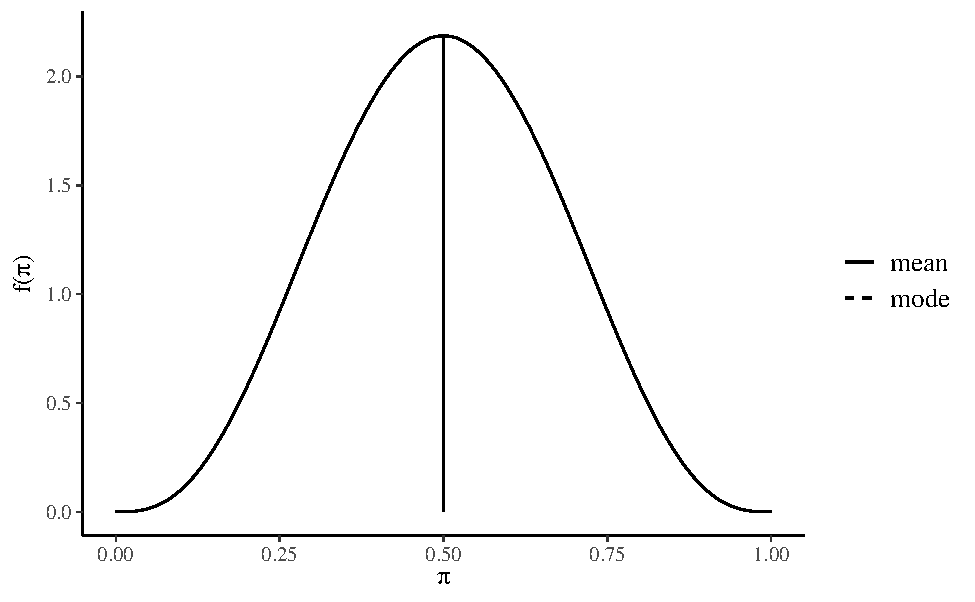
\includegraphics{ds4psy_files/figure-latex/unnamed-chunk-9-1} \end{center}

Possiamo quantificare la nostra incertezza calcolando, con un grado di fiducia del 95\%, la regione nella quale, in base a tale credenza a priori, si trova il valore del parametro. Per ottenere tale intervallo di credibilità a priori, usiamo la funzione \texttt{qbeta()} di \(\R\). In \texttt{qbeta()} i parametri \(\alpha\) e \(\beta\) sono chiamati \texttt{shape1} e \texttt{shape2}:

\begin{Shaded}
\begin{Highlighting}[]
\FunctionTok{qbeta}\NormalTok{(}\FunctionTok{c}\NormalTok{(}\FloatTok{0.025}\NormalTok{, }\FloatTok{0.975}\NormalTok{), }\AttributeTok{shape1 =} \DecValTok{4}\NormalTok{, }\AttributeTok{shape2 =} \DecValTok{4}\NormalTok{)}
\CommentTok{\#\textgreater{} [1] 0.1841 0.8159}
\end{Highlighting}
\end{Shaded}

Se poniamo \(\alpha=10\) e \(\beta=10\), questo corrisponde ad una credenza a priori che sia egualmente probabile per un'aspettativa futura essere distorta negativamente o positivamente,

\begin{Shaded}
\begin{Highlighting}[]
\FunctionTok{plot\_beta}\NormalTok{(}\AttributeTok{alpha =} \DecValTok{10}\NormalTok{, }\AttributeTok{beta =} \DecValTok{10}\NormalTok{, }\AttributeTok{mean =} \ConstantTok{TRUE}\NormalTok{, }\AttributeTok{mode =} \ConstantTok{TRUE}\NormalTok{)}
\end{Highlighting}
\end{Shaded}

\begin{center}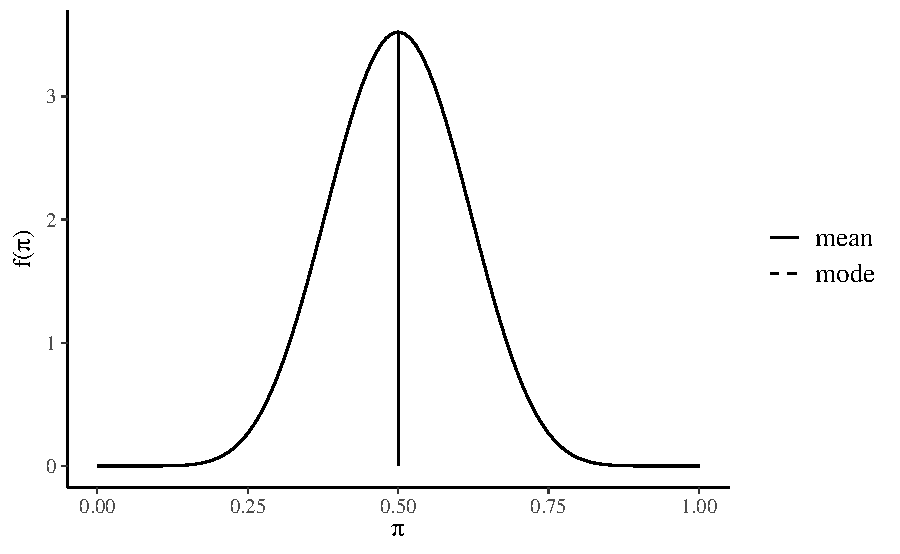
\includegraphics{ds4psy_files/figure-latex/unnamed-chunk-11-1} \end{center}

ma ora la nostra certezza a priori sul valore del parametro è maggiore, come indicato dall'intervallo al 95\%:

\begin{Shaded}
\begin{Highlighting}[]
\FunctionTok{qbeta}\NormalTok{(}\FunctionTok{c}\NormalTok{(}\FloatTok{0.025}\NormalTok{, }\FloatTok{0.975}\NormalTok{), }\AttributeTok{shape1 =} \DecValTok{10}\NormalTok{, }\AttributeTok{shape2 =} \DecValTok{10}\NormalTok{)}
\CommentTok{\#\textgreater{} [1] 0.2886 0.7114}
\end{Highlighting}
\end{Shaded}

Quale distribuzione a priori dobbiamo scegliere? In un problema concreto di analisi dei dati, la scelta della distribuzione a priori dipende dalle credenze a priori che vogliamo includere nell'analisi dei dati. Se non abbiamo alcuna informazione a priori, potremmo usare \(\alpha=1\) e \(\beta=1\), che produce una distribuzione a priori uniforme. Ma l'uso di distribuzioni a priori uniformi è sconsigliato per vari motivi, inclusa l'instabilità numerica della stima dei parametri. È meglio invece usare una distribuzione a priori poco informativa, come \(\mbox{Beta}(2, 2)\).

Nella discussione successiva, solo per fare un esempio, useremo quale distribuzione a priori una \(\mbox{Beta}(2, 10)\), ovvero:

\[
p(\theta) = \frac{\Gamma(12)}{\Gamma(2)\Gamma(10)}\theta^{2-1} (1-\theta)^{10-1}.
\]

\begin{Shaded}
\begin{Highlighting}[]
\FunctionTok{plot\_beta}\NormalTok{(}\AttributeTok{alpha =} \DecValTok{2}\NormalTok{, }\AttributeTok{beta =} \DecValTok{10}\NormalTok{, }\AttributeTok{mean =} \ConstantTok{TRUE}\NormalTok{, }\AttributeTok{mode =} \ConstantTok{TRUE}\NormalTok{)}
\end{Highlighting}
\end{Shaded}

\begin{center}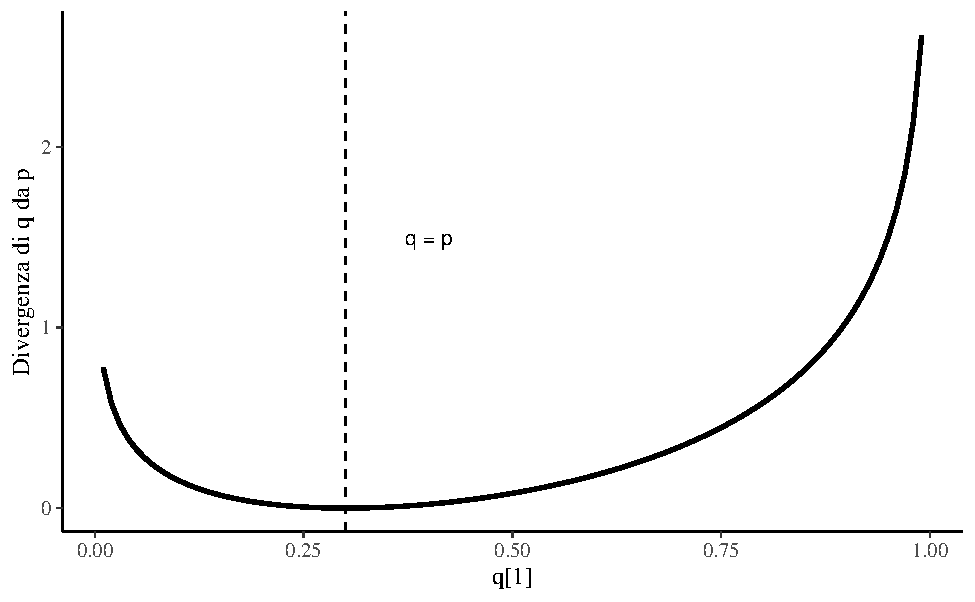
\includegraphics{ds4psy_files/figure-latex/unnamed-chunk-13-1} \end{center}

La \(\mbox{Beta}(2, 10)\) esprime la credenza che \(\theta < 0.5\), con il valore più plausibile pari a cicrca 0.1.

\hypertarget{la-specificazione-della-distribuzione-a-posteriori}{%
\subsection{La specificazione della distribuzione a posteriori}\label{la-specificazione-della-distribuzione-a-posteriori}}

Una volta scelta una distribuzione a priori di tipo Beta, i cui parametri rispecchiano le nostre credenze iniziali su \(\theta\), la distribuzione a posteriori viene specificata dalla formula di Bayes:

\[
\text{distribuzione a posteriori} = \frac{\text{verosimiglianza}\cdot\text{distribuzione a priori}}{\text{verosimiglianza marginale}}.
\]

Nel caso presente abbiamo

\[
p(\theta \mid n=30, y=23) = \frac{\Big[\binom{30}{23}\theta^{23}(1-\theta)^{30-23}\Big]\Big[\frac{\Gamma(12)}{\Gamma(2)\Gamma(10)}\theta^{2-1} (1-\theta)^{10-1}\Big]}{p(y = 23)},
\]

laddove \(p(y = 23)\), ovvero la verosimiglianza marginale, è una costante di normalizzazione che fa sì che l'area sottesa alla densità a posteriori sia unitaria.

Riscriviamo ora l'equazione precedente in termini generali

\[
p(\theta \mid n, y) = \frac{\Big[\binom{n}{y}\theta^{y}(1-\theta)^{n-y}\Big]\Big[\frac{\Gamma(a+b)}{\Gamma(a)\Gamma(b)}\theta^{a-1} (1-\theta)^{b-1}\Big]}{p(y)}
\]

e raccogliendo tutte le costanti otteniamo:

\[
p(\theta \mid n, y) =\left[\frac{\binom{n}{y}\frac{\Gamma(a+b)}{\Gamma(a)\Gamma(b)}}{p(y)}\right] \theta^{y}(1-\theta)^{n-y}\theta^{a-1} (1-\theta)^{b-1}.
\]

Se ignoriamo il termine costante all'interno della parentesi quadra

\begin{align}
p(\theta \mid n, y) &\propto \theta^{y}(1-\theta)^{n-y}\theta^{a-1} (1-\theta)^{b-1},\notag\\
&\propto \theta^{a+y-1}(1-\theta)^{b+n-y-1},\notag
\end{align}

il termine di destra dell'equazione precedente identifica il \emph{kernel} della distribuzione a posteriori e corrisponde ad una Beta \emph{non normalizzata} di parametri \(a + y\) e \(b + n - y\).

Per ottenere una distribuzione di densità, dobbiamo aggiungere una costante di normalizzazione al kernel della distribuzione a posteriori. In base alla definizione della distribuzione Beta, ed essendo \(a' = a+y\) e \(b' = b+n-y\), tale costante di normalizzazione sarà uguale a

\[
\frac{\Gamma(a'+b')}{\Gamma(a')\Gamma(b')} = \frac{\Gamma(a+b+n)}{\Gamma(a+y)\Gamma(b+n-y)}.
\]

In altri termini, la distribuzione a posteriori diventa una \(\mbox{Beta}(a+y, b+n-y)\):

\[
\mbox{Beta}(a+y, b+n-y) = \frac{\Gamma(a+b+n)}{\Gamma(a+y)\Gamma(b+n-y)} \theta^{a+y-1}(1-\theta)^{b+n-y-1}.
\]

Possiamo concludere dicendo che siamo partiti da una verosimiglianza \(\Bin(n = 30, y = 23 \mid \theta)\). Moltiplicando la verosimiglianza per la distribuzione a priori \(\theta \sim \mbox{Beta}(2, 10)\), abbiamo ottenuto la distribuzione a posteriori \(p(\theta \mid n, y) \sim \mbox{Beta}(25, 17)\). Questo è un esempio di analisi coniugata: la distribuzione a posteriori del parametro ha la stessa forma funzionale della distribuzione a priori. La presente combinazione di verosimiglianza e distribuzione a priori è chiamata caso coniugato \emph{Beta-Binomiale} ed è descritto dal seguente teorema.

\begin{theorem}
Sia data la funzione di verosimiglianza \(\Bin(n, y \mid \theta)\) e sia \(\mbox{Beta}(\alpha, \beta)\) una distribuzione a priori. In tali circostanze, la distribuzione a posteriori del parametro \(\theta\) sarà una distribuzione \(\mbox{Beta}(\alpha + y, \beta + n - y)\).
\end{theorem}

È facile calcolare il valore atteso a posteriori di \(\theta\). Essendo \(\E[\mbox{Beta}(\alpha, \beta)] = \frac{\alpha}{\alpha + \beta}\), il risultato cercato diventa

\begin{equation}
\E_{\text{post}} [\mathrm{Beta}(\alpha + y, \beta + n - y)] = \frac{\alpha + y}{\alpha + \beta +n}.
\label{eq:ev-post-beta-bin-1}
\end{equation}

\begin{exercise}

Usando le funzione \(\R\) \texttt{plot\_beta\_binomial()} e \texttt{plot\_beta\_binomial()} del pacchetto \texttt{bayesrules}, si rappresenti in maniera grafica e si descriva in forma numerica l'aggiornamento bayesiano Beta-Binomiale per i dati di \citet{zetschefuture2019}.

Per i dati in discussione, abbiamo:

\begin{Shaded}
\begin{Highlighting}[]
\NormalTok{bayesrules}\SpecialCharTok{::}\FunctionTok{plot\_beta\_binomial}\NormalTok{(}
  \AttributeTok{alpha =} \DecValTok{2}\NormalTok{, }\AttributeTok{beta =} \DecValTok{10}\NormalTok{, }\AttributeTok{y =} \DecValTok{23}\NormalTok{, }\AttributeTok{n =} \DecValTok{30}
\NormalTok{  ) }
\end{Highlighting}
\end{Shaded}

\begin{center}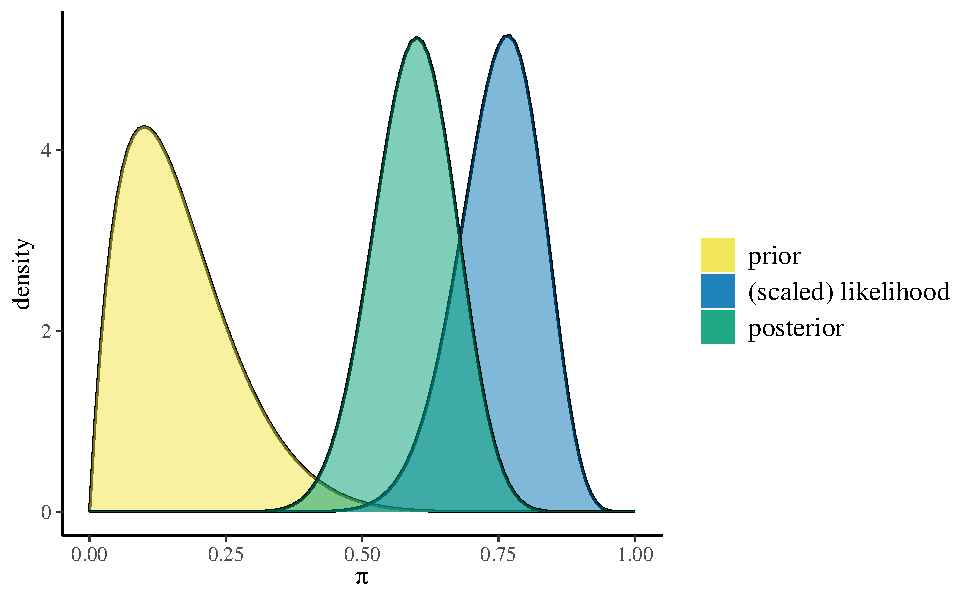
\includegraphics{ds4psy_files/figure-latex/unnamed-chunk-14-1} \end{center}

È facile replicare il grafico precedente scrivendo noi stessi una funzione, come descritto in Appendice \ref{appendix:beta-binom}. Con la funzione \texttt{plot\_beta\_binom()} e i dati usati in precedenza otteniamo

\begin{Shaded}
\begin{Highlighting}[]
\FunctionTok{plot\_beta\_bin}\NormalTok{(}\DecValTok{2}\NormalTok{, }\DecValTok{10}\NormalTok{, }\DecValTok{23}\NormalTok{, }\DecValTok{30}\NormalTok{)}
\end{Highlighting}
\end{Shaded}

\begin{center}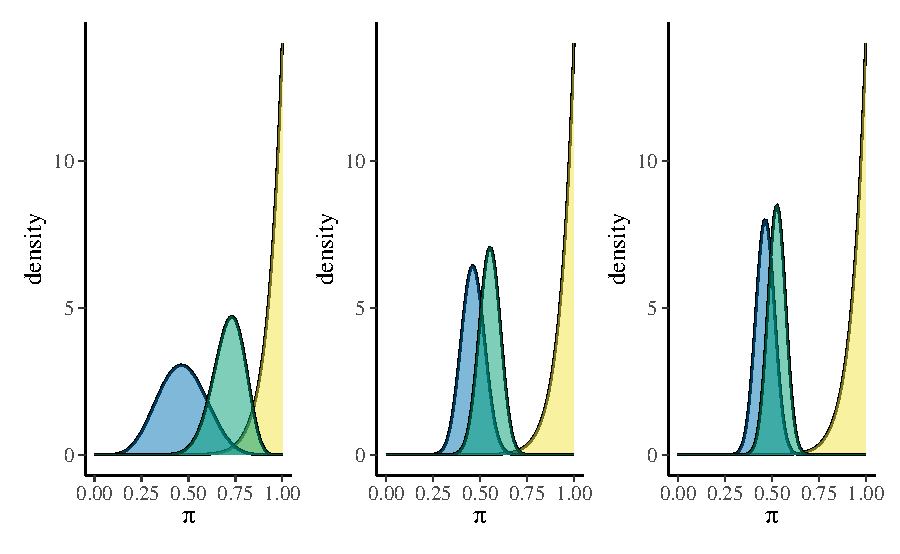
\includegraphics{ds4psy_files/figure-latex/unnamed-chunk-16-1} \end{center}

Un sommario delle distribuzioni a priori e a posteriori si ottiene usando la funzione \texttt{summarize\_beta\_binomial()}:

\begin{Shaded}
\begin{Highlighting}[]
\NormalTok{bayesrules}\SpecialCharTok{:::}\FunctionTok{summarize\_beta\_binomial}\NormalTok{(}
  \AttributeTok{alpha =} \DecValTok{2}\NormalTok{, }\AttributeTok{beta =} \DecValTok{10}\NormalTok{, }\AttributeTok{y =} \DecValTok{23}\NormalTok{, }\AttributeTok{n =} \DecValTok{30}
\NormalTok{)}
\CommentTok{\#\textgreater{}       model alpha beta   mean mode      var      sd}
\CommentTok{\#\textgreater{} 1     prior     2   10 0.1667  0.1 0.010684 0.10336}
\CommentTok{\#\textgreater{} 2 posterior    25   17 0.5952  0.6 0.005603 0.07485}
\end{Highlighting}
\end{Shaded}

\end{exercise}

\begin{exercise}

Per i dati di \citet{zetschefuture2019}, si trovino la media, la moda, la deviazione standard della distribuzione a posteriori di \(\theta\). Si trovi inoltre l'intervallo di credibilità a posteriori del 95\% per il parametro \(\theta\).

Usando la \ref{thm:beta-binom}, possiamo ottenere l'intervallo di credibilità a posteriori del 95\% per il parametro \(\theta\) come segue:

\begin{Shaded}
\begin{Highlighting}[]
\FunctionTok{qbeta}\NormalTok{(}\FunctionTok{c}\NormalTok{(}\FloatTok{0.025}\NormalTok{, }\FloatTok{0.975}\NormalTok{), }\AttributeTok{shape1 =} \DecValTok{25}\NormalTok{, }\AttributeTok{shape2 =} \DecValTok{17}\NormalTok{)}
\CommentTok{\#\textgreater{} [1] 0.4450 0.7368}
\end{Highlighting}
\end{Shaded}

La media della distribuzione a posteriori è

\begin{Shaded}
\begin{Highlighting}[]
\DecValTok{25} \SpecialCharTok{/}\NormalTok{ (}\DecValTok{25} \SpecialCharTok{+} \DecValTok{17}\NormalTok{)}
\CommentTok{\#\textgreater{} [1] 0.5952}
\end{Highlighting}
\end{Shaded}

La moda della distribuzione a posteriori è

\begin{Shaded}
\begin{Highlighting}[]
\NormalTok{(}\DecValTok{25} \SpecialCharTok{{-}} \DecValTok{1}\NormalTok{) }\SpecialCharTok{/}\NormalTok{ (}\DecValTok{25} \SpecialCharTok{+} \DecValTok{17} \SpecialCharTok{{-}} \DecValTok{2}\NormalTok{)}
\CommentTok{\#\textgreater{} [1] 0.6}
\end{Highlighting}
\end{Shaded}

La deviazione standard della distribuzione a priori è

\begin{Shaded}
\begin{Highlighting}[]
\FunctionTok{sqrt}\NormalTok{((}\DecValTok{25} \SpecialCharTok{*} \DecValTok{17}\NormalTok{) }\SpecialCharTok{/}\NormalTok{ ((}\DecValTok{25} \SpecialCharTok{+} \DecValTok{17}\NormalTok{)}\SpecialCharTok{\^{}}\DecValTok{2} \SpecialCharTok{*}\NormalTok{ (}\DecValTok{25} \SpecialCharTok{+} \DecValTok{17} \SpecialCharTok{+} \DecValTok{1}\NormalTok{)))}
\CommentTok{\#\textgreater{} [1] 0.07485}
\end{Highlighting}
\end{Shaded}

\end{exercise}

\begin{exercise}

Si trovino i parametri e le proprietà della distribuzione a posteriori del parametro \(\theta\) per i dati dell'esempio relativo alla ricerca di Stanley Milgram discussa da \citet{Johnson2022bayesrules}.

Nel 1963, Stanley Milgram presentò una ricerca sulla propensione delle persone a obbedire agli ordini di figure di autorità, anche quando tali ordini possono danneggiare altre persone \citep{milgram1963behavioral}. Nell'articolo, Milgram descrive lo studio come \emph{``consist{[}ing{]} of ordering a naive subject to administer electric shock to a victim. A simulated shock generator is used, with 30 clearly marked voltage levels that range from IS to 450 volts. The instrument bears verbal designations that range from Slight Shock to Danger: Severe Shock. The responses of the victim, who is a trained confederate of the experimenter, are standardized. The orders to administer shocks are given to the naive subject in the context of a `learning experiment' ostensibly set up to study the effects of punishment on memory. As the experiment proceeds the naive subject is commanded to administer increasingly more intense shocks to the victim, even to the point of reaching the level marked Danger: Severe Shock.''}

All'insaputa del partecipante, gli shock elettrici erano falsi e l'attore stava solo fingendo di provare il dolore dello shock.

\citet{Johnson2022bayesrules} fanno inferenza sui risultati dello studio di Milgram mediante il modello Beta-Binomiale. Il parametro di interesse è \(\theta\), la probabiltà che una persona obbedisca all'autorità (in questo caso, somministrando lo shock più severo), anche se ciò significa recare danno ad altri. \citet{Johnson2022bayesrules} ipotizzano che, prima di raccogliere dati, le credenze di Milgram relative a \(\theta\) possano essere rappresentate mediante una \(\mbox{Beta}(1, 10)\). Sia \(y = 26\) il numero di soggetti che, sui 40 partecipanti allo studio, aveva accettato di infliggere lo shock più severo. Assumendo che ogni partecipante si comporti indipendentemente dagli altri, possiamo modellare la dipendenza di \(y\) da \(\theta\) usando la distribuzione binomiale. Giungiamo dunque al seguente modello bayesiano Beta-Binomiale:

\begin{align}
y \mid \theta & \sim \Bin(n = 40, \theta) \notag\\
\theta & \sim \text{Beta}(1, 10) \; . \notag
\end{align}

Usando le funzioni di \texttt{bayesrules} possiamo facilmente calcolare i parametri e le proprietà della distribuzione a posteriori:

\begin{Shaded}
\begin{Highlighting}[]
\NormalTok{bayesrules}\SpecialCharTok{:::}\FunctionTok{summarize\_beta\_binomial}\NormalTok{(}
  \AttributeTok{alpha =} \DecValTok{1}\NormalTok{, }\AttributeTok{beta =} \DecValTok{10}\NormalTok{, }\AttributeTok{y =} \DecValTok{26}\NormalTok{, }\AttributeTok{n =} \DecValTok{40}
\NormalTok{)}
\CommentTok{\#\textgreater{}       model alpha beta    mean   mode      var      sd}
\CommentTok{\#\textgreater{} 1     prior     1   10 0.09091 0.0000 0.006887 0.08299}
\CommentTok{\#\textgreater{} 2 posterior    27   24 0.52941 0.5306 0.004791 0.06922}
\end{Highlighting}
\end{Shaded}

Il processo di aggiornamento bayesiano è descritto dalla figura seguente:

\begin{Shaded}
\begin{Highlighting}[]
\FunctionTok{plot\_beta\_bin}\NormalTok{(}\DecValTok{1}\NormalTok{, }\DecValTok{10}\NormalTok{, }\DecValTok{26}\NormalTok{, }\DecValTok{40}\NormalTok{)}
\end{Highlighting}
\end{Shaded}

\begin{center}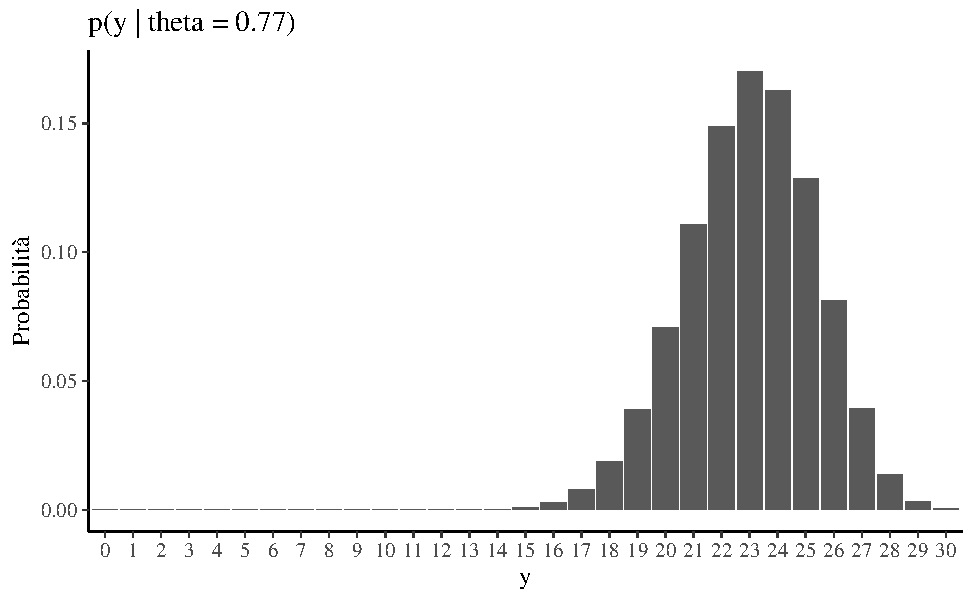
\includegraphics{ds4psy_files/figure-latex/unnamed-chunk-23-1} \end{center}

\end{exercise}

\hypertarget{principali-distribuzioni-coniugate}{%
\section{Principali distribuzioni coniugate}\label{principali-distribuzioni-coniugate}}

Esistono molte altre combinazioni simili di verosimiglianza e distribuzione a priori le quali producono una distribuzione a posteriori che ha la stessa densità della distribuzione a priori. Sono elencate qui sotto le più note coniugazioni tra modelli statistici e distribuzioni a priori.

\begin{itemize}
\tightlist
\item
  Per il modello Normale-Normale \(\mathcal{N}(\mu, \sigma^2_0)\), la distribizione iniziale è \(\mathcal{N}(\mu_0, \tau^2)\) e la distribuzione finale è \(\mathcal{N}\left(\frac{\mu_0\sigma^2 + \bar{y}n\tau^2}{\sigma^2 + n\tau^2}, \frac{\sigma^2\tau^2}{\sigma^2 + n\tau^2} \right)\).
\item
  Per il modello Poisson-gamma \(\text{Po}(\theta)\), la distribizione iniziale è \(\Gamma(\lambda, \delta)\) e la distribuzione finale è \(\Gamma(\lambda + n \bar{y}, \delta +n)\).
\item
  Per il modello esponenziale \(\text{Exp}(\theta)\), la distribizione iniziale è \(\Gamma(\lambda, \delta)\) e la distribuzione finale è \(\Gamma(\lambda + n, \delta +n\bar{y})\).
\item
  Per il modello uniforme-Pareto \(\text{U}(0, \theta)\), la distribizione iniziale è \(\mbox{Pa}(\alpha, \varepsilon)\) e la distribuzione finale è \(\mbox{Pa}(\alpha + n, \max(y_{(n)}, \varepsilon))\).
\end{itemize}

\hypertarget{commenti-e-considerazioni-finali-1}{%
\section*{Commenti e considerazioni finali}\label{commenti-e-considerazioni-finali-1}}


Lo scopo di questa discussione è stato quello di mostrare come sia possibile combinare le nostre conoscenze a priori (espresse nei termini di una densità di probabilità) con le evidenze fornite dai dati (espresse nei termini della funzione di verosimiglianza), così da determinare, mediante il teorema di Bayes, una distribuzione a posteriori, la quale condensa l'incertezza che abbiamo sul parametro \(\theta\). Per illustrare tale problema, abbiamo considerato una situazione nella quale \(\theta\) corrisponde alla probabilità di successo in una sequenza di prove Bernoulliane. Abbiamo visto come, in queste circostanze, sia ragionevole esprimere le nostre credenze a priori mediante la densità Beta, con opportuni parametri. L'inferenza rispetto ad una proporzione rappresenta un caso particolare, ovvero un caso nel quale la distribuzione a priori è Beta e la verosimiglianza è Binomiale. In tali circostanze, la distribuzione a posteriori diventa una distribuzione Beta -- questo è il cosiddetto modello Beta-Binomiale. Dato che utilizza una distribuzione a priori coniugata, dunque, il modello Beta-Binomiale rende possibile la determinazione analitica dei parametri della distribuzione a posteriori.

\mainmatter

\hypertarget{part-appendici}{%
\part{Appendici}\label{part-appendici}}

\hypertarget{appendix-appendici}{%
\appendix \addcontentsline{toc}{chapter}{\appendixname}}


\hypertarget{simbologia-di-base}{%
\chapter{Simbologia di base}\label{simbologia-di-base}}

Per una scrittura più sintetica possono essere utilizzati alcuni simboli matematici.

\begin{itemize}
\tightlist
\item
  \(\log(x)\): il logaritmo naturale di \(x\).
\item
  L'operatore logico booleano \(\land\) significa ``e'' (congiunzione forte) mentre il connettivo di disgiunzione \(\lor\) significa ``o'' (oppure) (congiunzione debole).
\item
  Il quantificatore esistenziale \(\exists\) vuol dire ``esiste almeno un'' e indica l'esistenza di almeno una istanza del concetto/oggetto indicato. Il quantificatore esistenziale di unicità \(\exists!\) (``esiste soltanto un'') indica l'esistenza di esattamente una istanza del concetto/oggetto indicato. Il quantificatore esistenziale \(\nexists\) nega l'esistenza del concetto/oggetto indicato.
\item
  Il quantificatore universale \(\forall\) vuol dire ``per ogni.''
\item
  \(\mathcal{A, S}\): insiemi.
\item
  \(x \in A\): \(x\) è un elemento dell'insieme \(A\).
\item
  L'implicazione logica ``\(\Rightarrow\)'' significa ``implica'' (se \ldots allora). \(P \Rightarrow Q\) vuol dire che \(P\) è condizione sufficiente per la verità di \(Q\) e che \(Q\) è condizione necessaria per la verità di \(P\).
\item
  L'equivalenza matematica ``\(\iff\)'' significa ``se e solo se'' e indica una condizione necessaria e sufficiente, o corrispondenza biunivoca.
\item
  Il simbolo \(\vert\) si legge ``tale che.''
\item
  Il simbolo \(\triangleq\) (o \(:=\)) si legge ``uguale per definizione.''
\item
  Il simbolo \(\Delta\) indica la differenza fra due valori della variabile scritta a destra del simbolo.
\item
  Il simbolo \(\propto\) si legge ``proporzionale a.''
\item
  Il simbolo \(\approx\) si legge ``circa.''
\item
  Il simbolo \(\in\) della teoria degli insiemi vuol dire ``appartiene'' e indica l'appartenenza di un elemento ad un insieme. Il simbolo \(\notin\) vuol dire ``non appartiene.''
\item
  Il simbolo \(\subseteq\) si legge ``è un sottoinsieme di'' (può coincidere con l'insieme stesso). Il simbolo \(\subset\) si legge ``è un sottoinsieme proprio di.''
\item
  Il simbolo \(\#\) indica la cardinalità di un insieme.
\item
  Il simbolo \(\cap\) indica l'intersezione di due insiemi. Il simbolo \(\cup\) indica l'unione di due insiemi.
\item
  Il simbolo \(\emptyset\) indica l'insieme vuoto o evento impossibile.
\item
  In matematica, \(\mbox{argmax}\) identifica l'insieme dei punti per i quali una data funzione raggiunge il suo massimo. In altre parole, \(\mbox{argmax}_x f(x)\) è l'insieme dei valori di \(x\) per i quali \(f(x)\) raggiunge il valore più alto.
\item
  \(a, c, \alpha, \gamma\): scalari.
\item
  \(\boldsymbol{x}, \boldsymbol{y}\): vettori.
\item
  \(\boldsymbol{X}, \boldsymbol{Y}\): matrici.
\item
  \(X \sim p\): la variabile casuale \(X\) si distribuisce come \(p\).
\item
  \(p(\cdot)\): distribuzione di massa o di densità di probabilità.
\item
  \(p(y \mid \boldsymbol{x})\): la probabilità o densità di \(y\) dato \(\boldsymbol{x}\), ovvero \(p(y = \boldsymbol{Y} \mid x = \boldsymbol{X})\).
\item
  \(f(x)\): una funzione arbitraria di \(x\).
\item
  \(f(\boldsymbol{X}; \theta, \gamma)\): \(f\) è una funzione di \(\boldsymbol{X}\) con parametri \(\theta, \gamma\). Questa notazione indica che \(\boldsymbol{X}\) sono i dati che vengono passati ad un modello di parametri \(\theta, \gamma\).
\item
  \(\mathcal{N}(\mu, \sigma^2)\): distribuzione gaussiana di media \(\mu\) e varianza \(sigma^2\).
\item
  \(\mbox{Beta}(\alpha, \beta)\): distribuzione Beta di parametri \(\alpha\) e \(\beta\).
\item
  \(\mathcal{U}(a, b)\): distribuzione uniforme con limite inferiore \(a\) e limite superiore \(b\).
\item
  \(\mbox{Cauchy}(\alpha, \beta)\): distribuzione di Cauchy di parametri \(\alpha\) (posizione: media) e \(\beta\) (scala: radice quadrata della varianza).
\item
  \(\mathcal{B}(p)\): distribuzione di Bernoulli di parametro \(p\) (probabilità di successo).
\item
  \(\mbox{Bin}(n, p)\): distribuzione binomiale di parametri \(n\) (numero di prove) e \(p\) (probabilità di successo).
\item
  \(\mathbb{KL} (p \mid\mid q)\): la divergenza di Kullback-Leibler da \(p\) a \(q\).
\end{itemize}

\hypertarget{numeri-binari-interi-razionali-irrazionali-e-reali}{%
\chapter{Numeri binari, interi, razionali, irrazionali e reali}\label{numeri-binari-interi-razionali-irrazionali-e-reali}}

\hypertarget{numeri-binari}{%
\section{Numeri binari}\label{numeri-binari}}

I numeri più semplici sono quelli binari, cioè zero o uno. Useremo spesso numeri binari per indicare se qualcosa è vero o falso, presente o assente. I numeri binari sono molto utili per ottenere facilmente delle statistiche riassuntive in \(\R\).Supponiamo di chiedere a 10 studenti ``Ti piacciono i mirtilli?'' Poniamo che le risposte siano le seguenti:

\begin{Shaded}
\begin{Highlighting}[]
\NormalTok{opinion }\OtherTok{\textless{}{-}} \FunctionTok{c}\NormalTok{(}
  \StringTok{"Yes"}\NormalTok{, }\StringTok{"No"}\NormalTok{, }\StringTok{"Yes"}\NormalTok{, }\StringTok{"No"}\NormalTok{, }\StringTok{"Yes"}\NormalTok{, }\StringTok{"No"}\NormalTok{, }\StringTok{"Yes"}\NormalTok{,}
  \StringTok{"Yes"}\NormalTok{, }\StringTok{"Yes"}\NormalTok{, }\StringTok{"Yes"}
\NormalTok{)}
\NormalTok{opinion}
\CommentTok{\#\textgreater{}  [1] "Yes" "No"  "Yes" "No"  "Yes" "No"  "Yes" "Yes"}
\CommentTok{\#\textgreater{}  [9] "Yes" "Yes"}
\end{Highlighting}
\end{Shaded}

Tali risposte possono essere ricodificate nei termini di valori di verità, ovvero, vero e falso, generalmente denotati rispettivamente come 1 e 0. In \(\R\) tale ricodifica può essere effettuata mediante l'operatore \texttt{==} che è un test per l'uguaglianza e restituisce il valore logico VERO se i due oggetti valutati sono uguali e FALSO se non lo sono:

\begin{Shaded}
\begin{Highlighting}[]
\NormalTok{opinion }\OtherTok{\textless{}{-}}\NormalTok{ opinion }\SpecialCharTok{==} \StringTok{"Yes"}
\NormalTok{opinion}
\CommentTok{\#\textgreater{}  [1]  TRUE FALSE  TRUE FALSE  TRUE FALSE  TRUE  TRUE}
\CommentTok{\#\textgreater{}  [9]  TRUE  TRUE}
\end{Highlighting}
\end{Shaded}

R considera i valori di verità e i numeri binari in modo equivalente, con TRUE uguale a 1 e FALSE uguale a zero. Di conseguenza, possiamo effettuare operazioni algebriche sui valori logici VERO e FALSO. Nell'esempio, possiamo sommare i valori di verità e dividere per 10

\begin{Shaded}
\begin{Highlighting}[]
\FunctionTok{sum}\NormalTok{(opinion) }\SpecialCharTok{/} \FunctionTok{length}\NormalTok{(opinion)}
\CommentTok{\#\textgreater{} [1] 0.7}
\end{Highlighting}
\end{Shaded}

in modo tale da calcolare una propozione, il che ci consente di concludere che 7 risposte su 10 sono positive.

\hypertarget{numeri-interi}{%
\section{Numeri interi}\label{numeri-interi}}

Un numero intero è un numero senza decimali. Si dicono \textbf{naturali} i numeri che servono a contare, come 1, 2, \ldots{} L'insieme dei numeri naturali si indica con il simbolo \(\mathbb{N}\). È anche necessario introdurre i numeri con il segno per poter trattare grandezze negative. Si ottengono così l'insieme numerico dei numeri interi relativi: \(\mathbb{Z} = \{0, \pm 1, \pm 2, \dots \}\)

\hypertarget{numeri-razionali}{%
\section{Numeri razionali}\label{numeri-razionali}}

I numeri razionali sono i numeri frazionari \(m/n\), dove \(m, n \in N\), con \(n \neq 0\). Si ottengono così i numeri razionali: \(\mathbb{Q} = \{\frac{m}{n} \,\vert\, m, n \in \mathbb{Z}, n \neq 0\}\). È evidente che \(\mathbb{N} \subseteq \mathbb{Z} \subseteq \mathbb{Q}\). Anche in questo caso è necessario poter trattare grandezze negative. I numeri razionali non negativi sono indicati con \(\mathbb{Q^+} = \{q \in \mathbb{Q} \,\vert\, q \geq 0\}\).

\hypertarget{numeri-irrazionali}{%
\section{Numeri irrazionali}\label{numeri-irrazionali}}

Tuttavia, non tutti i punti di una retta \(r\) possono essere rappresentati mediante i numeri interi e razionali. È dunque necessario introdurre un'altra classe di numeri. Si dicono \emph{irrazionali}, e sono denotati con \(\mathbb{R}\), i numeri che possono essere scritti come una frazione \(a / b\), con \(a\) e \(b\) interi e \(b\) diverso da 0. I numeri irrazionali sono i numeri illimitati e non periodici che quindi non possono essere espressi sotto forma di frazione. Per esempio, \(\sqrt{2}\), \(\sqrt{3}\) e \({\displaystyle \pi =3,141592\ldots}\) sono numeri irrazionali.

\hypertarget{numeri-reali}{%
\section{Numeri reali}\label{numeri-reali}}

I punti della retta \(r\) sono quindi ``di più'' dei numeri razionali. Per poter rappresentare tutti i punti della retta abbiamo dunque bisogno dei numeri \emph{reali}. I numeri reali possono essere positivi, negativi o nulli e comprendono, come casi particolari, i numeri interi, i numeri razionali e i numeri irrazionali. Spesso in statisticac il numero dei decimali indica il grado di precisione della misurazione.

\hypertarget{intervalli}{%
\section{Intervalli}\label{intervalli}}

Un intervallo si dice chiuso se gli estremi sono compresi nell'intervallo, aperto se gli estremi non sono compresi. Le caratteristiche degli intervalli sono riportate nella tabella seguente.

\begin{longtable}[]{@{}cll@{}}
\toprule
Intervallo & & \\
\midrule
\endhead
chiuso & \([a, b]\) & \(a \leq x \leq b\) \\
aperto & \((a, b)\) & \(a < x < b\) \\
chiuso a sinistra e aperto a destra & \([a, b)\) & \(a \leq x < b\) \\
aperto a sinistra e chiuso a destra & \((a, b]\) & \(a < x \leq b\) \\
\bottomrule
\end{longtable}

\hypertarget{insiemistica}{%
\chapter{Insiemi}\label{insiemistica}}

Un insieme (o collezione, classe, gruppo, \ldots) è un concetto primitivo, ovvero è un concetto che già possediamo. Georg Cantor l'ha definito nel modo seguente: \emph{un insieme è una collezione di oggetti, determinati e distinti, della nostra percezione o del nostro pensiero, concepiti come un tutto unico; tali oggetti si dicono elementi dell'insieme.}

Mentre non è rilevante la natura degli oggetti che costituiscono l'insieme, ciò che importa è distinguere se un dato oggetto appartenga o meno ad un insieme. Deve essere vera una delle due possibilità: il dato oggetto è un elemento dell'insieme considerato oppure non è elemento dell'insieme considerato. Due insiemi \(A\) e \(B\) si dicono uguali se sono formati dagli stessi elementi, anche se disposti in ordine diverso: \(A=B\). Due insiemi \(A\) e \(B\) si dicono diversi se non contengono gli stessi elementi: \(A \neq B\). Ad esempio, i seguenti insiemi sono uguali:

\[
\{1, 2, 3\} = \{3, 1, 2\} = \{1, 3, 2\}= \{1, 1, 1, 2, 3, 3, 3\}.
\]

Gli insiemi sono denotati da una lettera maiuscola, mentre le lettere minuscole, di solito, designano gli elementi di un insieme. Per esempio, un generico insieme \(A\) si indica con

\[
A = \{a_1, a_2, \dots, a_n\}, \quad \text{con~} n > 0.
\]

La scrittura \(a \in A\) dice che \(a\) è un elemento di \(A\). Per dire che \(b\) non è un elemento di \(A\) si scrive \(b \notin A.\)

Per quegli insiemi i cui elementi soddisfano una certa proprietà che li caratterizza, tale proprietà può essere usata per descrivere più sinteticamente l'insieme:

\[
A = \{x ~\vert~ \text{proprietà posseduta da~} x\},
\]

che si legge come ``\(A\) è l'insieme degli elementi \(x\) per cui è vera la proprietà indicata.'' Per esempio, per indicare l'insieme \(A\) delle coppie di numeri reali \((x,y)\) che appartengono alla parabola \(y = x^2 + 1\) si può scrivere:

\[
A = \{(x,y) ~\vert~ y = x^2 + 1\}.
\]

Dati due insiemi \(A\) e \(B\), diremo che \(A\) è un \emph{sottoinsieme} di \(B\) se e solo se tutti gli elementi di \(A\) sono anche elementi di \(B\):

\[
A \subseteq B \iff (\forall x \in A \Rightarrow x \in B).
\]

Se esiste almeno un elemento di \(B\) che non appartiene ad \(A\) allora diremo che \(A\) è un \emph{sottoinsieme proprio} di \(B\):

\[
A \subset B \iff (A \subseteq B, \exists~ x \in B ~\vert~ x \notin A).
\]

Un altro insieme, detto \emph{insieme delle parti}, o insieme potenza, che si associa all'insieme \(A\) è l'insieme di tutti i sottoinsiemi di \(A\), inclusi l'insieme vuoto e \(A\) stesso. Per esempio, per l'insieme \(A = \{a, b, c\}\), l'insieme delle parti è:

\[
\mathcal{P}(A) = \{
\emptyset, \{a\}, \{b\}, \{c\},
 \{a, b\}, \{a, c\}, \{c, b\},
 \{a, b, c\}
\}.
\]

\hypertarget{operazioni-tra-insiemi}{%
\section{Operazioni tra insiemi}\label{operazioni-tra-insiemi}}

Si definisce \emph{intersezione} di \(A\) e \(B\) l'insieme \(A \cap B\) di tutti gli elementi \(x\) che appartengono ad \(A\) e contemporaneamente a \(B\):

\[
A \cap B = \{x ~\vert~ x \in A \land x \in B\}.
\]

Si definisce \emph{unione} di \(A\) e \(B\) l'insieme \(A \cup B\) di tutti gli elementi \(x\) che appartengono ad \(A\) o a \(B\), cioè

\[
A \cup B = \{x ~\vert~ x \in A \lor x \in B\}.
\]

\emph{Differenza}. Si indica con \(A \setminus B\) l'insieme degli elementi di \(A\) che non appartengono a \(B\):

\[
A \setminus B = \{x ~\vert~ x \in A \land x \notin B\}.
\]

\emph{Insieme complementare}. Nel caso che sia \(B \subseteq A\), l'insieme differenza \(A \setminus B\) è detto insieme complementare di \(B\) in \(A\) e si indica con \(B^C\).

Dato un insieme \(S\), una \emph{partizione} di \(S\) è una collezione di sottoinsiemi di \(S\), \(S_1, \dots, S_k\), tali che

\[
S = S_1 \cup S_2 \cup \dots S_k
\]

e

\[
S_i \cap S_j, \quad \text{con~} i \neq j.
\]

La relazione tra unione, intersezione e insieme complementare è data dalle leggi di DeMorgan:

\[
(A \cup B)^c = A^c \cap B^c,
\] \[
(A \cap B)^c = A^c \cup B^c.
\]

\hypertarget{diagrammi-di-eulero-venn}{%
\section{Diagrammi di Eulero-Venn}\label{diagrammi-di-eulero-venn}}

In molte situazioni è utile servirsi dei cosiddetti diagrammi di Eulero-Venn per rappresentare gli insiemi e verificare le proprietà delle operazioni tra insiemi (si veda la figura \ref{fig:sets-venn-diagrams}. I diagrammi di Venn sono così nominati in onore del matematico inglese del diciannovesimo secolo John Venn anche se Leibnitz e Eulero avevano già in precedenza utilizzato rappresentazioni simili. In tale rappresentazione, gli insiemi sono individuati da regioni del piano delimitate da una curva chiusa. Nel caso di insiemi finiti, è possibile evidenziare esplicitamente alcuni elementi di un insieme mediante punti, quando si possono anche evidenziare tutti gli elementi degli insiemi considerati.

\begin{figure}[h]

{\centering 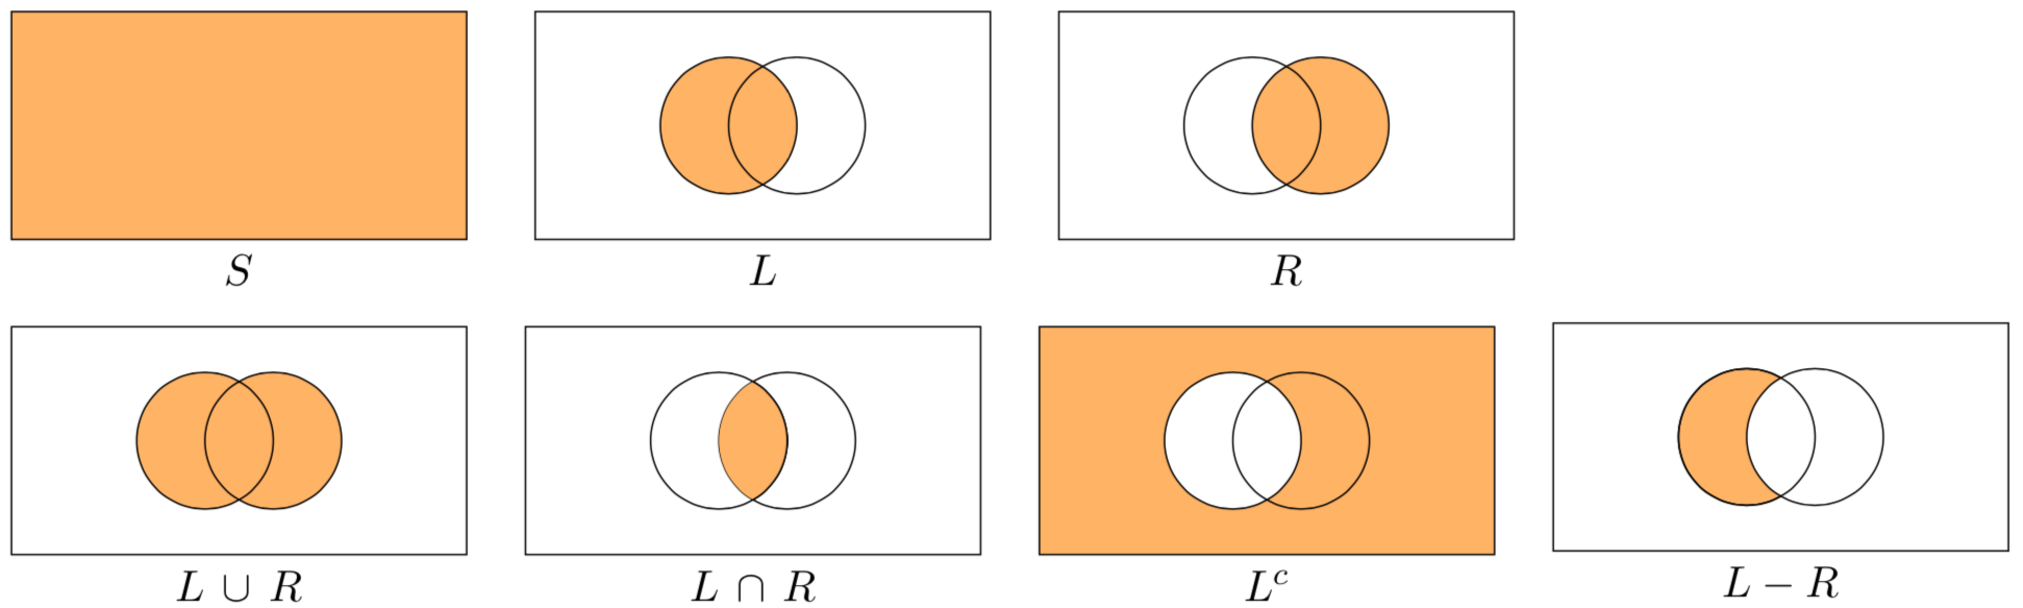
\includegraphics[width=1\linewidth]{images/sets-venn-diagrams} 

}

\caption{In tutte le figure $S$ è la regione delimitata dal rettangolo, $L$ è la regione all'interno del cerchio di sinistra e $R$ è la regione all'interno del cerchio di destra. La regione evidenziata mostra l'insieme indicato sotto ciascuna figura.}\label{fig:sets-venn-diagrams}
\end{figure}

I diagrammi di Eulero-Venn che forniscono una dimostrazione delle leggi di DeMorgan sono forniti nella figura \ref{fig:demorgan}.

\begin{figure}[h]

{\centering 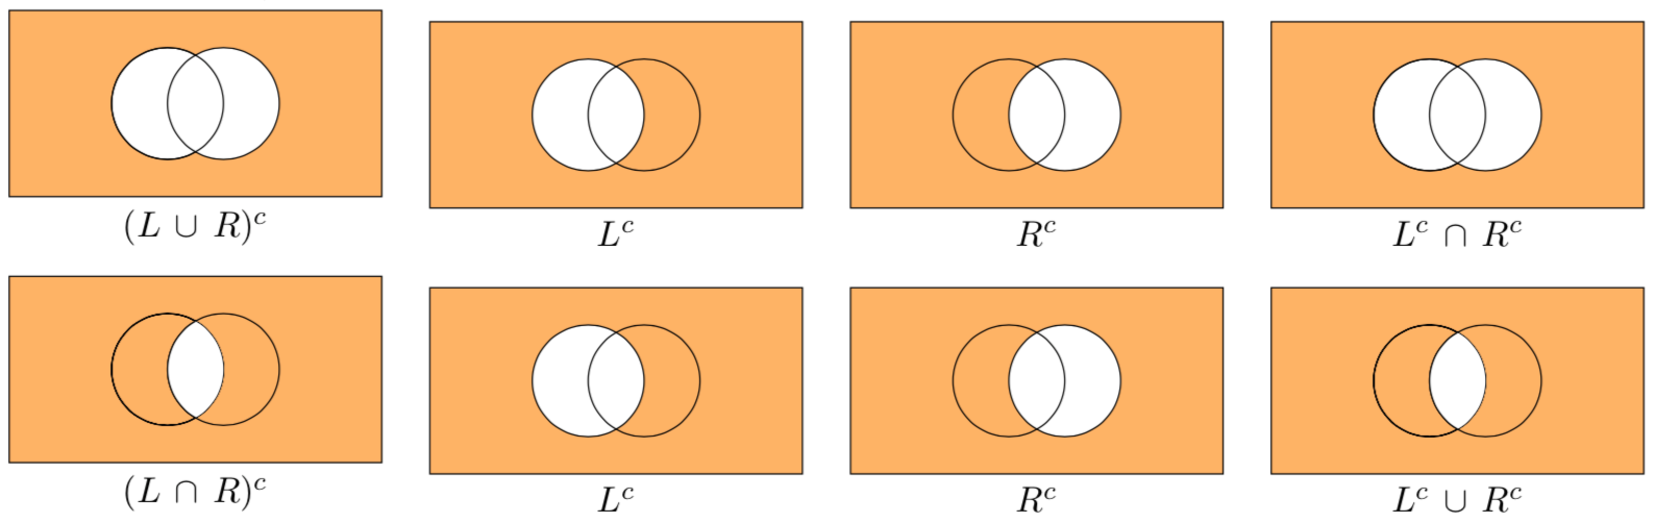
\includegraphics[width=1\linewidth]{images/demorgan} 

}

\caption{Dimostrazione delle leggi di DeMorgan.}\label{fig:demorgan}
\end{figure}

\hypertarget{coppie-ordinate-e-prodotto-cartesiano}{%
\section{Coppie ordinate e prodotto cartesiano}\label{coppie-ordinate-e-prodotto-cartesiano}}

Una coppia ordinata \((x,y)\) è l'insieme i cui elementi sono \(x \in A\) e \(y \in B\) e nella quale \(x\) è la prima componente (o prima coordinata), \(y\) la seconda. L'insieme di tutte le coppie ordinate costruite a partire dagli insiemi \(A\) e \(B\) viene detto \textbf{prodotto cartesiano}:

\[
A \times B = \{(x, y) ~\vert~ x \in A \land y \in B\}.
\]

Ad esempio, sia \(A = \{1, 2, 3\}\) e \(B = \{a, b\}\). Allora,

\[
\{1, 2\} \times \{a, b, c\} = \{(1, a), (1, b), (1, c), (2, a), (2, b), (2, c)\}.
\]

\hypertarget{cardinalituxe0}{%
\section{Cardinalità}\label{cardinalituxe0}}

Si definisce \emph{cardinalità} (o potenza) di un insieme finito il numero degli elementi dell'insieme. Viene indicata con \(\vert A\vert, \#(A)\) o \(\text{c}(A)\).

\hypertarget{sommatorie}{%
\chapter{Simbolo di somma (sommatorie)}\label{sommatorie}}

Le somme si incontrano costantemente in svariati contesti matematici e statistici quindi abbiamo bisogno di una notazione adeguata che ci consenta di gestirle. La somma dei primi \(n\) numeri interi può essere scritta come \(1+2+\dots+(n-1)+n\), dove `\(\dots\)' ci dice di completare la sequenza definita dai termini che vengono prima e dopo. Ovviamente, una notazione come \(1+7+\dots+73.6\) non avrebbe alcun senso senza qualche altro tipo di precisazione. In generale, nel seguito incontreremo delle somme nella forma

\begin{equation}
x_1+x_2+\dots+x_n,\notag
\end{equation}

dove \(x_i\) è un numero che è stato definito altrove. La notazione precedente, che fa uso dei tre puntini di sospensione, è utile in alcuni contesti ma in altri risulta ambigua. Pertanto la notazione di uso corrente è del tipo

\begin{equation}
  \sum_{i=1}^n x_i\notag
\end{equation}

e si legge ``sommatoria per \(i\) che va da \(1\) a \(n\) di \(x_i\)''. Il simbolo \(\sum\) (lettera sigma maiuscola dell'alfabeto greco) indica l'operazione di somma, il simbolo \(x_i\) indica il generico addendo della sommatoria, le lettere \(1\) ed \(n\) indicano i cosiddetti \emph{estremi della sommatoria}, ovvero l'intervallo (da \(1\) fino a \(n\) estremi inclusi) in cui deve variare l'indice \(i\) allorché si sommano gli addendi \(x_i\). Solitamente l'estremo inferiore è \(1\) ma potrebbe essere qualsiasi altri numero \(m < n\). Quindi

\[
  \sum_{i=1}^n x_i = x_1 + x_{2} + \dots + x_{n}.
\]

Per esempio, se i valori \(x\) sono \(\{3, 11, 4, 7\}\), si avrà

\[
  \sum_{i=1}^4 x_i = 3+11+4+7 = 25 
\]

laddove \(x_1 = 3\), \(x_2 = 11\), eccetera. La quantità \(x_i\) nella formula precedente si dice l'\emph{argomento} della sommatoria, mentre la variabile \(i\), che prende i valori naturali successivi indicati nel simbolo, si dice \emph{indice} della sommatoria.

La notazione di sommatoria può anche essere fornita nella forma seguente

\begin{equation}
  \sum_{P(i)} x_i\notag
\end{equation}

dove \(P(i)\) è qualsiasi proposizione riguardante \(i\) che può essere vera o falsa. Quando è ovvio che si vogliono sommare tutti i valori di \(n\) osservazioni, la notazione può essere semplificata nel modo seguente: \(\sum_{i} x_i\) oppure \(\sum x_i\). Al posto di \(i\) si possono trovare altre lettere: \(k, j, l, \dots\),.

\hypertarget{manipolazione-di-somme}{%
\section{Manipolazione di somme}\label{manipolazione-di-somme}}

È conveniente utilizzare le seguenti regole per semplificare i calcoli che coinvolgono l'operatore della sommatoria.

\hypertarget{proprietuxe0-1}{%
\subsection{Proprietà 1}\label{proprietuxe0-1}}

La sommatoria di \(n\) valori tutti pari alla stessa costante \(a\) è pari a \(n\) volte la costante stessa:

\[
  \sum_{i=1}^{n} a =  \underbrace{a + a + \dots + a}_{n~\text{volte}} = n a.
  \]

\hypertarget{proprietuxe0-2-proprietuxe0-distributiva}{%
\subsection{Proprietà 2 (proprietà distributiva)}\label{proprietuxe0-2-proprietuxe0-distributiva}}

Nel caso in cui l'argomento contenga una costante, è possibile riscrivere la sommatoria. Ad esempio con

\[
  \sum_{i=1}^{n} a x_i =  a x_1 + a x_2 + \dots + a x_n
  \]

è possibile raccogliere la costante \(a\) e fare \(a(x_1 +x_2 + \dots + x_n)\). Quindi possiamo scrivere

\[
  \sum_{i=1}^{n} a x_i =  a  \sum_{i=1}^{n} x_i.
  \]

\hypertarget{proprietuxe0-3-proprietuxe0-associativa}{%
\subsection{Proprietà 3 (proprietà associativa)}\label{proprietuxe0-3-proprietuxe0-associativa}}

Nel caso in cui

\[
  \sum_{i=1}^{n} (a + x_i) =  (a + x_1) +  (a + x_1) + \dots  (a + x_n)
  \]

si ha che

\[
  \sum_{i=1}^{n} (a + x_i) =  n a + \sum_{i=1}^{n} x_i.
  \]

È dunque chiaro che in generale possiamo scrivere

\[
  \sum_{i=1}^{n} (x_i + y_i) =  \sum_{i=1}^{n} x_i + \sum_{i=1}^{n} y_i.
  \]

\hypertarget{proprietuxe0-4}{%
\subsection{Proprietà 4}\label{proprietuxe0-4}}

Se deve essere eseguita un'operazione algebrica (innalzamento a potenza, logaritmo, ecc.) sull'argomento della sommatoria, allora tale operazione algebrica deve essere eseguita prima della somma. Per esempio,

\[
\sum_{i=1}^{n} x_i^2 = x_1^2 + x_2^2 + \dots + x_n^2 \neq \left(\sum_{i=1}^{n} x_i \right)^2.
\]

\hypertarget{proprietuxe0-5}{%
\subsection{Proprietà 5}\label{proprietuxe0-5}}

Nel caso si voglia calcolare \(\sum_{i=1}^{n} x_i y_i\), il prodotto tra i punteggi appaiati deve essere eseguito prima e la somma dopo:

\[
\sum_{i=1}^{n} x_i y_i = x_1 y_1 + x_2 y_2 + \dots + x_n y_n,
\]

infatti, \(a_1 b_1 + a_2 b_2 \neq (a_1 + a_2)(b_1 + b_2)\).

\hypertarget{doppia-sommatoria}{%
\section{Doppia sommatoria}\label{doppia-sommatoria}}

È possibile incontrare la seguente espressione in cui figurano una doppia sommatoria e un doppio indice:

\[
\sum_{i=1}^{n}\sum_{j=1}^{m} x_{ij}.
\]

La doppia sommatoria comporta che per ogni valore dell'indice esterno, \(i\) da \(1\) ad \(n\), occorre sviluppare la seconda sommatoria per \(j\) da \(1\) ad \(m\). Quindi,

\[
\sum_{i=1}^{3}\sum_{j=4}^{6} x_{ij} = (x_{1, 4} + x_{1, 5} + x_{1, 6}) + (x_{2, 4} + x_{2, 5} + x_{2, 6}) + (x_{3, 4} + x_{3, 5} + x_{3, 6}).
\]

Un caso particolare interessante di doppia sommatoria è il seguente:

\[
\sum_{i=1}^{n}\sum_{j=1}^{n} x_i y_j
\]

Si può osservare che nella sommatoria interna (quella che dipende dall'indice \(j\)), la quantità \(x_i\) è costante, ovvero non dipende dall'indice (che è \(j\)). Allora possiamo estrarre \(x_i\) dall'operatore di sommatoria interna e scrivere

\[
\sum_{i=1}^{n} \left( x_i \sum_{j=1}^{n} y_j \right).
\]

Allo stesso modo si può osservare che nell'argomento della sommatoria esterna la quantità costituita dalla sommatoria in \(j\) non dipende dall'indice \(i\) e quindi questa quantità può essere estratta dalla sommatoria esterna. Si ottiene quindi

\[
\sum_{i=1}^{n}\sum_{j=1}^{n} x_i y_j = \sum_{i=1}^{n} \left( x_i \sum_{j=1}^{n} y_j \right) = \sum_{i=1}^{n}\ x_i \sum_{j=1}^{n} y_j.
\]

\begin{exercise}
Si verifichi quanto detto sopra nel caso particolare di \(x = \{2, 3, 1\}\) e \(y = \{1, 4, 9\}\), svolgendo prima la doppia sommatoria per poi verificare che quanto così ottenuto sia uguale al prodotto delle due sommatorie.

\begin{align}
\sum_{i=1}^3 \sum_{j=1}^3 x_i y_j &= x_1y_1 + x_1y_2 + x_1y_3 + 
x_2y_1 + x_2y_2 + x_2y_3 + 
x_3y_1 + x_3y_2 + x_3y_3 \notag\\
&= 2 \times (1+4+9) + 3 \times (1+4+9) + 2 \times (1+4+9) = 84,\notag
\end{align}

ovvero

\[
(2 + 3 + 1) \times (1+4+9) = 84.
\]
\end{exercise}

\hypertarget{sommatorie-e-produttorie-e-operazioni-vettoriali-in-r}{%
\section{\texorpdfstring{Sommatorie (e produttorie) e operazioni vettoriali in \texttt{R}}{Sommatorie (e produttorie) e operazioni vettoriali in R}}\label{sommatorie-e-produttorie-e-operazioni-vettoriali-in-r}}

Si noti che la notazione

\[
\sum_{n=0}^4 3n
\]

non è altro che un ciclo \texttt{for}:

\begin{Shaded}
\begin{Highlighting}[]
\NormalTok{sum }\OtherTok{\textless{}{-}} \DecValTok{0}
\ControlFlowTok{for}\NormalTok{ (n }\ControlFlowTok{in} \DecValTok{0}\SpecialCharTok{:}\DecValTok{4}\NormalTok{) \{}
\NormalTok{  sum }\OtherTok{=}\NormalTok{ sum }\SpecialCharTok{+} \DecValTok{3} \SpecialCharTok{*}\NormalTok{ n}
\NormalTok{\}}
\NormalTok{sum}
\CommentTok{\#\textgreater{} [1] 30}
\end{Highlighting}
\end{Shaded}

In maniera equivalente, e più semplice, possiamo scrivere

\begin{Shaded}
\begin{Highlighting}[]
\FunctionTok{sum}\NormalTok{(}\DecValTok{3} \SpecialCharTok{*}\NormalTok{ (}\DecValTok{0}\SpecialCharTok{:}\DecValTok{4}\NormalTok{))}
\CommentTok{\#\textgreater{} [1] 30}
\end{Highlighting}
\end{Shaded}

Allo stesso modo, la notazione

\[
\prod_{n=1}^{4} 2n
\] è anch'essa equivalente al ciclo \texttt{for}

\begin{Shaded}
\begin{Highlighting}[]
\NormalTok{prod }\OtherTok{\textless{}{-}} \DecValTok{1}
\ControlFlowTok{for}\NormalTok{ (n }\ControlFlowTok{in} \DecValTok{1}\SpecialCharTok{:}\DecValTok{4}\NormalTok{) \{}
\NormalTok{  prod }\OtherTok{\textless{}{-}}\NormalTok{ prod }\SpecialCharTok{*} \DecValTok{2} \SpecialCharTok{*}\NormalTok{ n}
\NormalTok{\}}
\NormalTok{prod}
\CommentTok{\#\textgreater{} [1] 384}
\end{Highlighting}
\end{Shaded}

che si può scrivere, più semplicemente, come

\begin{Shaded}
\begin{Highlighting}[]
\FunctionTok{prod}\NormalTok{(}\DecValTok{2} \SpecialCharTok{*}\NormalTok{ (}\DecValTok{1}\SpecialCharTok{:}\DecValTok{4}\NormalTok{))}
\CommentTok{\#\textgreater{} [1] 384}
\end{Highlighting}
\end{Shaded}

In entrambi i casi precedenti, abbiamo sostituito le operazioni aritmetiche eseguite all'interno di un ciclo \texttt{for} con le stesse operazioni aritmetiche eseguite sui vettori elemento per elemento.

\hypertarget{appendix:bayes-updating}{%
\chapter{Aggiornamento Bayesiano}\label{appendix:bayes-updating}}

Per fornire un esempio di aggiornamento bayesiano, consideriamo il seguente problema. Supponiamo che, per qualche strano errore di produzione, una fabbrica produca due tipi di monete. Il primo tipo di monete ha la caratteristica che, quando una moneta viene lanciata, la probabilità di osservare l'esito ``testa'' è 0.6. Per semplicità, sia \(\theta\) la probabilità di osservare l'esito ``testa''. Per una moneta del primo tipo, dunque, \(\theta = 0.6\). Per una moneta del secondo tipo, invece, la probabilità di produrre l'esito ``testa'' è 0.4. Ovvero, \(\theta = 0.4\).

Noi possediamo una moneta, ma non sappiamo se è del primo tipo o del secondo tipo. Sappiamo solo che il 75\% delle monete sono del primo tipo e il 25\% sono del secondo tipo. Sulla base di questa conoscenza \emph{a priori} -- ovvero sulla base di una conoscenza ottenuta senza avere eseguitol'esperimento che consiste nel lanciare la moneta una serie di volte per osservare gli esiti prodotti -- possiamo dire che la probabilità di una prima ipotesi, secondo la quale \(\theta = 0.6\), è 3 volte più grande della probabilità di una seconda ipotesi, secondo la quale \(\theta = 0.4\). Senza avere eseguito alcun esperimento casuale con la moneta, questo è quello che sappiamo.

Ora immaginiamo di lanciare una moneta due volte e di ottenere il risultato seguente: \(\{T, C\}\). Quello che ci chiediamo è: sulla base di questa evidenza, come cambiano le probabilità che associamo alle due ipotesi? In altre parole, ci chiediamo qual è la probabilità di ciascuna ipotesi alla luce dei dati che sono stati osservati: \(P(H \mid y)\), laddove \(y\) sono i dati osservati. Tale probabilità si chiama probabilità a posteriori. Inoltre, se confrontiamo le due ipotesi, ci chiediamo quale valore assuma il rapporto \(\frac{P(H_1 \mid y)}{P(H_2 \mid y)}\). Tale rapporto ci dice quanto è più probabile \(H_1\) rispetto ad \(H_2\), alla luce dei dati osservati. Infine, ci chiediamo come cambia il rapporto definito sopra, quando osserviamo via via nuovi risultati prodotti dal lancio della moneta.

Definiamo il problema in maniera più chiara. Conosciamo le probabilità a priori, ovvero \(P(H_1) = 0.75\) e \(P(H_1) = 0.25\). Quello che vogliamo conoscere sono le probabilità a posteriori \(P(H_1 \mid y)\) e \(P(H_2 \mid y)\). Per trovare le probabilità a posteriori applichiamo il teorema di Bayes:

\[
\begin{split}
P(H_1 \mid y) &= \frac{P(y \mid H_1) P(H_1)}{P(y)} \\
&= \frac{P(y \mid H_1) P(H_1)}{P(y \mid H_1) P(H_1) + P(y \mid H_2) P(H_2)},
\end{split}
\]

laddove lo sviluppo del denominatore deriva da un'applicazione del teorema della probabilità totale. Inoltre,

\[
P(H_2 \mid y) = \frac{P(y \mid H_2) P(H_2)}{P(y \mid H_1) P(H_1) + P(y \mid H_2) P(H_2)}.
\]

Se consideriamo l'ipotesi \(H_1\) = ``la probabilità di testa è 0.6'', allora la verosimiglianza dei dati \(\{T, C\}\), ovvero la probabilità di osservare questa specifica sequenza di T e C, è uguale a \(0.6 \times 0.4 = 0.24.\) Dunque, \(P(y \mid H_1) = 0.24\).

Se invece consideriamo l'ipotesi \(H_2\) = ``la probabilità di testa è 0.4'', allora la verosimiglianza dei dati \(\{T, C\}\) è \(0.4 \times 0.6 = 0.24\), ovvero, \(P(y \mid H_2) = 0.24\). In base alle due ipotesi \(H_1\) e \(H_2\), dunque, i dati osservati hanno la medesima plausibilità di essere osservati. Per semplicità, calcoliamo anche

\[
\begin{split}
P(y) &= P(y \mid H_1) P(H_1) + P(y \mid H_2) P(H_2) \\
&= 0.24 \cdot 0.75 + 0.24 \cdot 0.25 \\
&= 0.24.
\end{split}
\]

Le probabilità a posteriori diventano:

\[
\begin{split}
P(H_1 \mid y) &= \frac{P(y \mid H_1) P(H_1)}{P(y)}\\
&= \frac{0.24 \cdot 0.75}{0.24} \\
&= 0.75,
\end{split}
\]

\[
\begin{split}
P(H_2 \mid y) &= \frac{P(y \mid H_2) P(H_2)}{P(y)} \\
&= \frac{0.24 \cdot 0.25}{0.24} \\
&= 0.25.
\end{split}
\]

Possiamo dunque concludere dicendo che, sulla base dei dati osservati, l'ipotesi \(H_1\) ha una probabilità 3 volte maggiore di essere vera dell'ipotesi \(H_2\).

È tuttavia possibile raccogliere più evidenze e, sulla base di esse, le probabilità a posteriori cambieranno. Supponiamo di lanciare la moneta una terza volta e di osservare croce. I nostri dati dunque sono \(\{T, C, C\}\).

Di conseguenza, \(P(y \mid H_1) = 0.6 \cdot 0.4 \cdot 0.4 = 0.096\) e \(P(y \mid H_2) = 0.4 \cdot 0.6 \cdot 0.6 = 0.144\). Ne segue che le probabilità a posteriori diventano:

\[
\begin{split}
P(H_1 \mid y) &= \frac{P(y \mid H_1) P(H_1)}{P(y)} \\
&= \frac{0.096 \cdot 0.75}{0.096 \cdot 0.75 + 0.144 \cdot 0.25} \\
&= 0.667,
\end{split}
\]

\[
\begin{split}
P(H_2 \mid y) &= \frac{P(y \mid H_2) P(H_2)}{P(y)} \\
&= \frac{0.144 \cdot 0.25}{0.096 \cdot 0.75 + 0.144 \cdot 0.25} \\
&= 0.333.
\end{split}
\]

In queste circostanze, le evidenze che favoriscono \(H_1\) nei confronti di \(H_2\) sono solo pari ad un fattore di 2.

Se otteniamo ancora croce in un quarto lancio della moneta, i nostri dati diventano: \(\{T, C, C, C\}\). Ripetendo il ragionamento fatto sopra, \(P(y \mid H_1) = 0.6 \cdot 0.4 \cdot 0.4 \cdot 0.4 = 0.0384\) e \(P(y \mid H_2) = 0.4 \cdot 0.6 \cdot 0.6 \cdot 0.6 = 0.0864\). Dunque

\begin{equation}
P(H_1 \mid y) = \frac{0.0384 \cdot 0.75}{0.0384 \cdot 0.75 + 0.0864 \cdot 0.25} = 0.571,\notag
\end{equation}

\begin{equation}
P(H_2 \mid y) = \frac{0.0864 \cdot 0.25}{0.0384 \cdot 0.75 + 0.0864 \cdot 0.25} = 0.429.\notag
\end{equation}

e le evidenze a favore di \(H_1\) si riducono a 1.33. Se si ottenesse un altro esito croce in un sesto lancio della moneta, l'ipotesi \(H2\) diventerebbe più probabile dell'ipotesi \(H_1\).

In conclusione, questo esercizio ci fa capire come sia possibile aggiornare le nostre credenze sulla base delle evidenze disponibili, ovvero come sia possibile passare da un grado di conoscenza del mondo a priori a una conoscenza a posteriori. Se prima di lanciare la moneta ritenevamo che l'ipotesi \(H_1\) fosse tre volte più plausibile dell'ipotesi \(H_2\), dopo avere osservato uno specifico campione di dati siamo giunti alla conclusione opposta. Il processo di aggiornamento bayesiano, dunque, ci fornisce un metodo per modificare il livello di fiducia in una data ipotesi, alla luce di nuove informazioni.

\hypertarget{appendix:exrc-abs-prob}{%
\chapter{Il teorema della probabilità assoluta}\label{appendix:exrc-abs-prob}}

\begin{exercise}
Consideriamo un'urna che contiene 5 palline rosse e 2 palline verdi. Due palline vengono estratte, una dopo l'altra. Vogliamo sapere la probabilità dell'evento ``la seconda pallina estratta è rossa''.

Lo spazio campionario è \(\Omega = \{RR, RV, VR, VV\}\). Chiamiamo \(R_1\) l'evento ``la prima pallina estratta è rossa'', \(V_1\) l'evento ``la prima pallina estratta è verde'', \(R_2\) l'evento ``la seconda pallina estratta è rossa'' e \(V_2\) l'evento ``la seconda pallina estratta è verde''. Dobbiamo trovare \(P(R_2)\) e possiamo risolvere il problema usando il teorema della probabilità assoluta \eqref{eq:prob-total-1b}:

\[
\begin{split}
P(R_2) &= P(R_2 \mid R_1) P(R_1) + P(R_2 \mid V_1)P(V_1)\\
&= \frac{4}{6} \cdot \frac{5}{7} + \frac{5}{6} \cdot \frac{2}{7} \\
&= \frac{30}{42} = \frac{5}{7}.
\end{split}
\]

Se la prima estrazione è quella di una pallina rossa, nell'urna restano 4 palline rosse e due verdi, dunque, la probabilità che la seconda estrazione produca una pallina rossa è uguale a 4/6. La probabilità di una pallina rossa nella prima estrazione è 5/7. Se la prima estrazione è quella di una pallina verde, nell'urna restano 5 palline rosse e una pallina verde, dunque, la probabilità che la seconda estrazione produca una pallina rossa è uguale a 5/6. La probabilità di una pallina verde nella prima estrazione è 2/7.
\end{exercise}

\hypertarget{funs-exp-log}{%
\chapter{Esponenziali e logaritmi}\label{funs-exp-log}}

\hypertarget{potenze-ad-esponente-reale}{%
\section*{Potenze ad esponente reale}\label{potenze-ad-esponente-reale}}


Per un qualsiasi numero razionale \(\frac{m}{n}\) (in cui \(n > 0\)) si ha

\[
a^{\frac{m}{n}} = \sqrt[n]{a^m}
\] per numeri \(a\) reali positivi.

\hypertarget{proprietuxe0}{%
\subsection*{Proprietà}\label{proprietuxe0}}


Se \(a\), \(b\) sono reali positivi ed \(x\), \(y\) reali qualsiasi, si ha

\begin{itemize}
\tightlist
\item
  \(a^0 = 1\) e \(a^{-x} = \frac{1}{a^x}\),
\item
  \(a^x a^y = a^{x+y}\) e \(\frac{a^x}{a^y} = a^{x-y}\),
\item
  \(a^x b^x = (ab)^{x}\) e \(\frac{a^x}{b^x} = \left(\frac{a}{b}\right)^x\),
\item
  \((a^x)^y = a^{xy}\).
\end{itemize}

\hypertarget{funzione-esponenziale}{%
\section{Funzione esponenziale}\label{funzione-esponenziale}}

\begin{definition}
La funzione esponenziale con base \(a\) è \begin{equation}
f(x) = a^x
\end{equation}

dove \(a > 0\), \(a \neq 1\) e \(x\) è qualsiasi numero reale.
\end{definition}

La base \(a = 1\) è esclusa perché produce \(f(x) = 1^x = 1\), la quale è una costante, non una funzione esponenziale.

Per esempio, un grafico della funzione esponenziale di base 2 si trova con

\begin{Shaded}
\begin{Highlighting}[]
\NormalTok{exp\_base2 }\OtherTok{=} \ControlFlowTok{function}\NormalTok{(x)\{}\DecValTok{2}\SpecialCharTok{\^{}}\NormalTok{x\}}
\FunctionTok{tibble}\NormalTok{(}\AttributeTok{x =} \FunctionTok{c}\NormalTok{(}\SpecialCharTok{{-}}\DecValTok{5}\NormalTok{, }\DecValTok{5}\NormalTok{)) }\SpecialCharTok{\%\textgreater{}\%}
\FunctionTok{ggplot}\NormalTok{(}\FunctionTok{aes}\NormalTok{(}\AttributeTok{x =}\NormalTok{ x)) }\SpecialCharTok{+}
  \FunctionTok{stat\_function}\NormalTok{(}\AttributeTok{fun =}\NormalTok{ exp\_base2)}
\end{Highlighting}
\end{Shaded}

\begin{center}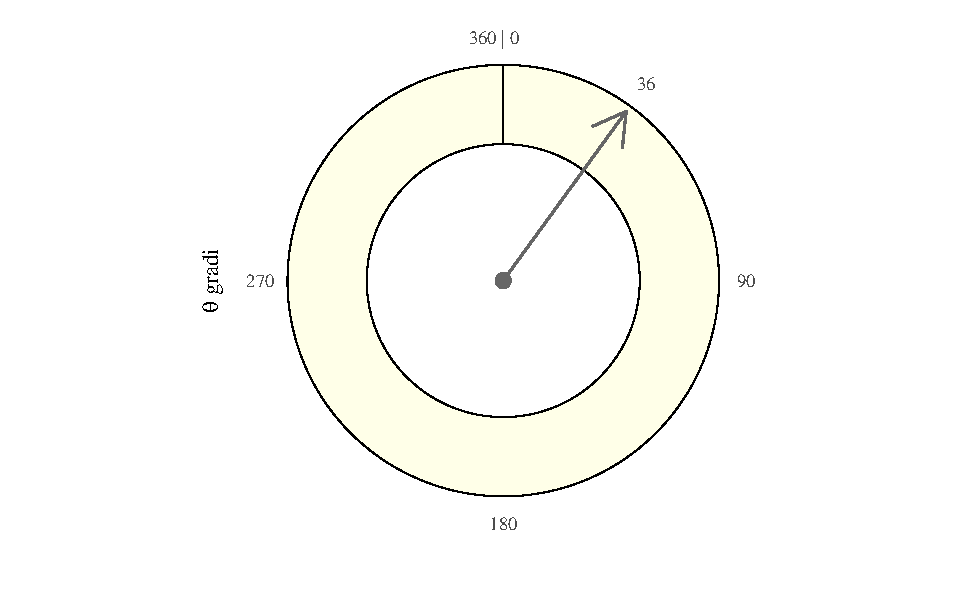
\includegraphics{ds4psy_files/figure-latex/unnamed-chunk-32-1} \end{center}

Se usiamo la base 4 troviamo

\begin{Shaded}
\begin{Highlighting}[]
\NormalTok{exp\_base4 }\OtherTok{=} \ControlFlowTok{function}\NormalTok{(x)\{}\DecValTok{4}\SpecialCharTok{\^{}}\NormalTok{x\}}
\FunctionTok{tibble}\NormalTok{(}\AttributeTok{x =} \FunctionTok{c}\NormalTok{(}\SpecialCharTok{{-}}\DecValTok{5}\NormalTok{, }\DecValTok{5}\NormalTok{)) }\SpecialCharTok{\%\textgreater{}\%}
\FunctionTok{ggplot}\NormalTok{(}\FunctionTok{aes}\NormalTok{(}\AttributeTok{x =}\NormalTok{ x)) }\SpecialCharTok{+}
  \FunctionTok{stat\_function}\NormalTok{(}\AttributeTok{fun =}\NormalTok{ exp\_base4)}
\end{Highlighting}
\end{Shaded}

\begin{center}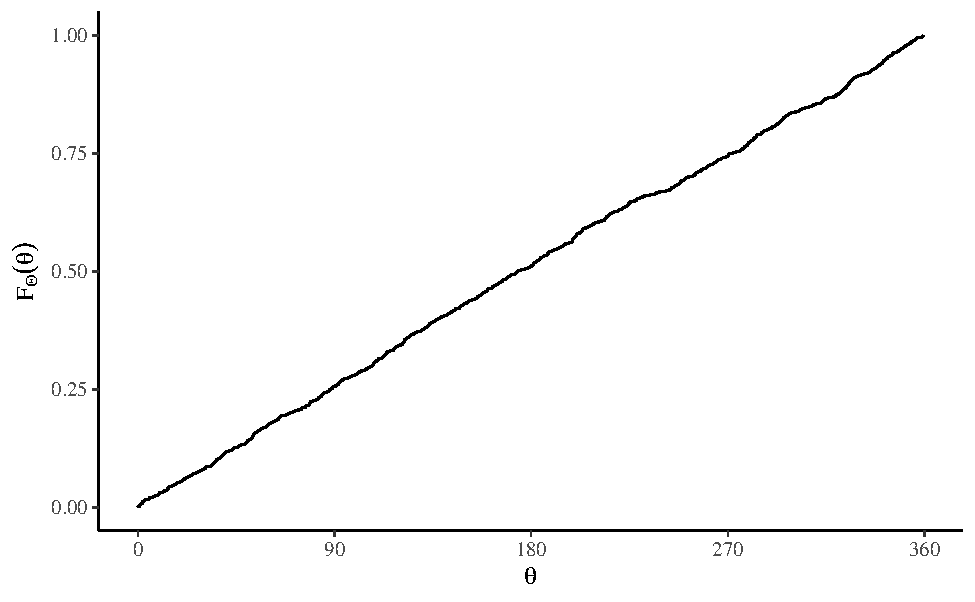
\includegraphics{ds4psy_files/figure-latex/unnamed-chunk-33-1} \end{center}

Oppure

\begin{Shaded}
\begin{Highlighting}[]
\NormalTok{exp\_base4 }\OtherTok{=} \ControlFlowTok{function}\NormalTok{(x)\{}\DecValTok{4}\SpecialCharTok{\^{}{-}}\NormalTok{\{x\}\}}
\FunctionTok{tibble}\NormalTok{(}\AttributeTok{x =} \FunctionTok{c}\NormalTok{(}\SpecialCharTok{{-}}\DecValTok{5}\NormalTok{, }\DecValTok{5}\NormalTok{)) }\SpecialCharTok{\%\textgreater{}\%}
\FunctionTok{ggplot}\NormalTok{(}\FunctionTok{aes}\NormalTok{(}\AttributeTok{x =}\NormalTok{ x)) }\SpecialCharTok{+}
  \FunctionTok{stat\_function}\NormalTok{(}\AttributeTok{fun =}\NormalTok{ exp\_base4)}
\end{Highlighting}
\end{Shaded}

\begin{center}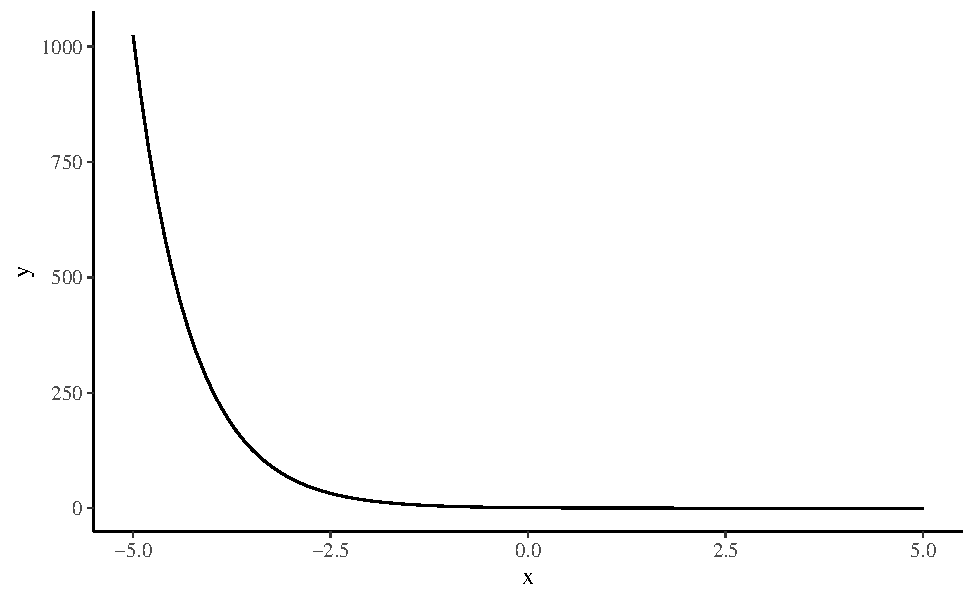
\includegraphics{ds4psy_files/figure-latex/unnamed-chunk-34-1} \end{center}

In molte applicazioni la scelta più conveniente per la base è il numero irrazionale \(e = 2.718281828\dots\). Questo numero è chiamato la \emph{base naturale}. La funzione \(f(x) = e^x\) è chiamata \emph{funzione esponenziale naturale}.

Per esempio, abbiamo

\begin{Shaded}
\begin{Highlighting}[]
\NormalTok{exp\_base\_e}\OtherTok{=} \ControlFlowTok{function}\NormalTok{(x)\{}\FunctionTok{exp}\NormalTok{(x)\}}
\FunctionTok{tibble}\NormalTok{(}\AttributeTok{x =} \FunctionTok{c}\NormalTok{(}\SpecialCharTok{{-}}\DecValTok{2}\NormalTok{, }\FloatTok{1.5}\NormalTok{)) }\SpecialCharTok{\%\textgreater{}\%}
\FunctionTok{ggplot}\NormalTok{(}\FunctionTok{aes}\NormalTok{(}\AttributeTok{x =}\NormalTok{ x)) }\SpecialCharTok{+}
  \FunctionTok{stat\_function}\NormalTok{(}\AttributeTok{fun =}\NormalTok{ exp\_base\_e)}
\end{Highlighting}
\end{Shaded}

\begin{center}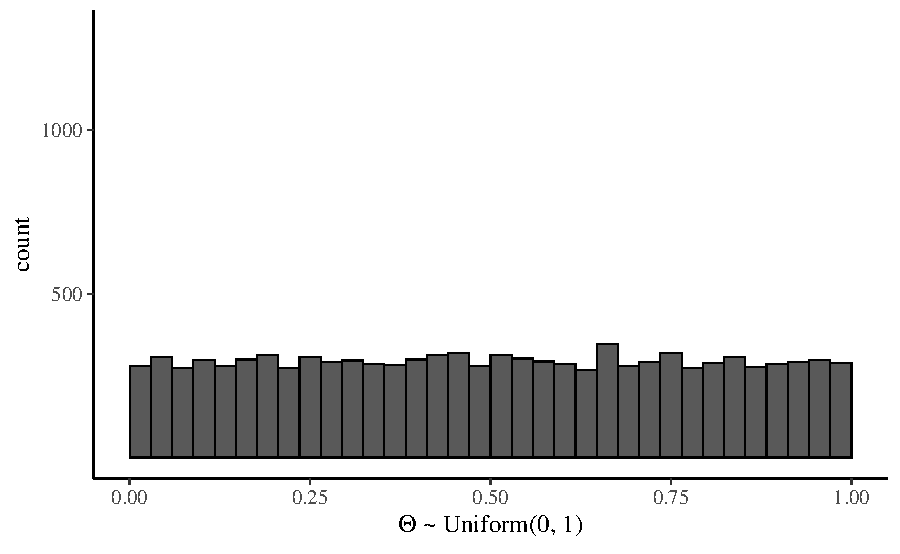
\includegraphics{ds4psy_files/figure-latex/unnamed-chunk-35-1} \end{center}

\hypertarget{logaritmi}{%
\section*{Logaritmi}\label{logaritmi}}


Dati due numeri reali \(b > 0\) e \(a > 0\) con \(a \neq 1\), l'equazione esponenziale \(a^x = b\) ammette sempre una ed una sola soluzione. Tale soluzione è detta \emph{logaritmo in base \(a\) di \(b\)} ed è indicata con la scrittura \(\log_a b\), dove \(b\) è detto \emph{argomento} del logaritmo. In altri termini, per definizione si ha

\[
x = \log_a b \Longleftrightarrow a^x = b
\]

\[
\text{dove deve essere } a > 0, \ a \neq 1,\ b > 0.
\]

Quando valutiamo i logaritmi, dobbiamo ricordare che un logaritmo è un esponente: il logaritmo in base \(a\) di \(b\), \(\log_a b\), è l'esponente da attribuire alla base \(a\) per ottenere l'argomento \(b\). Le seguenti equazioni sono dunque equivalenti:

\begin{equation}
y = \log_a x \qquad x = a^y.\notag
\end{equation}

La prima equazione è in forma logaritmica e la seconda è in forma esponenziale. Ad esempio, l'equazione logaritmica \(2 = \log_3 9\) può essere riscritta in forma esponenziale come \(9 = 3^2\).

\begin{example}

Scrivendo l'argomento come potenza della base si ottiene

\begin{itemize}
\tightlist
\item
  \(\log_2 8 = \log_2 2^3 = 3\)
\item
  \(\log_3 \sqrt[7]{3^{20}} = \log_3 3^{\frac{20}{7}} = \frac{20}{7}\)
\item
  \(\log_{0.1} 0.01 = \log_{\frac{1}{10}}\frac{1}{100} = \log_{\frac{1}{10}}\left(\frac{1}{10}\right)^2 = 2\)
\end{itemize}

\end{example}

\hypertarget{proprietuxe0-2}{%
\subsection*{Proprietà}\label{proprietuxe0-2}}


Nell'operare con i logaritmi si procede spesso mediante le loro proprietà, che costituiscono una rilettura in termini di logaritmi delle proprietà delle potenze: se \(a\), \(b\) sono numeri reali positivi diversi da 1 ed \(x\), \(y\) reali positivi qualunque, allora

\begin{itemize}
\tightlist
\item
  \(\log_a (xy) = \log_a x + \log_a y\),
\item
  \(\log_a \left(\frac{x}{y}\right) = \log_a x - \log_a y\),
\item
  \(\log_a \left(x^{\alpha}\right) = \alpha \log_a x, \quad \forall \alpha \ \text{reale}\),
\item
  \(\log_a x = \frac{\log_b x}{\log_b a}\) (cambiamento di base).
\end{itemize}

\begin{example}
\begin{align}
\log_a (x+1) -\log_a x - 2 \log_a 2 &= \log_a (x+1) - (\log_a x+ \log_a 2^2)\notag\\
&= \log_a (x+1) - \log_a 4x\notag\\
&= \log_a \frac{x+1}{4x}.\notag
\end{align}
\end{example}

\hypertarget{funzione-logaritmica}{%
\section{Funzione logaritmica}\label{funzione-logaritmica}}

La funzione logaritmica è la funzione inversa della funzione esponenziale.

\begin{definition}
Siano \(a > 0\), \(a \neq 1\). Per \(x > 0\)

\begin{equation}
y = \log_a x \quad \text{se e solo se } x = a^y.
\end{equation}

La funzione data da

\begin{equation}
f(x) = \log_a x
\end{equation}

è chiamata funzione logaritmica.
\end{definition}

Per esempio, abbiamo

\begin{Shaded}
\begin{Highlighting}[]
\NormalTok{log\_funct }\OtherTok{\textless{}{-}} \ControlFlowTok{function}\NormalTok{(x)\{}
  \FunctionTok{log}\NormalTok{(x)}
\NormalTok{\}}
\FunctionTok{ggplot}\NormalTok{(}\FunctionTok{tibble}\NormalTok{(}\AttributeTok{x =} \FunctionTok{c}\NormalTok{(}\SpecialCharTok{{-}}\FloatTok{0.5}\NormalTok{, }\DecValTok{4}\NormalTok{)), }\FunctionTok{aes}\NormalTok{(}\AttributeTok{x =}\NormalTok{ x)) }\SpecialCharTok{+}
  \FunctionTok{stat\_function}\NormalTok{(}\AttributeTok{fun =}\NormalTok{ log\_funct) }\SpecialCharTok{+} 
  \FunctionTok{xlim}\NormalTok{(}\FunctionTok{c}\NormalTok{(}\SpecialCharTok{{-}}\DecValTok{1}\NormalTok{, }\DecValTok{4}\NormalTok{)) }\SpecialCharTok{+} 
  \FunctionTok{ylim}\NormalTok{(}\SpecialCharTok{{-}}\DecValTok{3}\NormalTok{, }\DecValTok{3}\NormalTok{) }\SpecialCharTok{+}
  \FunctionTok{labs}\NormalTok{(}\AttributeTok{x =} \StringTok{"}\SpecialCharTok{\textbackslash{}n}\StringTok{ x"}\NormalTok{, }\AttributeTok{y =} \StringTok{"y }\SpecialCharTok{\textbackslash{}n}\StringTok{"}\NormalTok{) }\SpecialCharTok{+}
  \FunctionTok{annotate}\NormalTok{(}\StringTok{"text"}\NormalTok{, }\AttributeTok{x =} \DecValTok{3}\NormalTok{, }\AttributeTok{y =} \DecValTok{3}\NormalTok{, }\AttributeTok{parse =} \ConstantTok{TRUE}\NormalTok{, }\AttributeTok{size =} \DecValTok{5}\NormalTok{, }\AttributeTok{fontface =} \StringTok{"bold"}\NormalTok{,}
           \AttributeTok{label=}\StringTok{"y == log(x)"}\NormalTok{) }\SpecialCharTok{+} 
  \FunctionTok{geom\_hline}\NormalTok{(}\AttributeTok{yintercept =} \DecValTok{0}\NormalTok{, }\AttributeTok{colour =} \StringTok{"gray"}\NormalTok{) }\SpecialCharTok{+}
  \FunctionTok{geom\_vline}\NormalTok{(}\AttributeTok{xintercept =} \DecValTok{0}\NormalTok{, }\AttributeTok{colour =} \StringTok{"gray"}\NormalTok{)}
\end{Highlighting}
\end{Shaded}

\begin{center}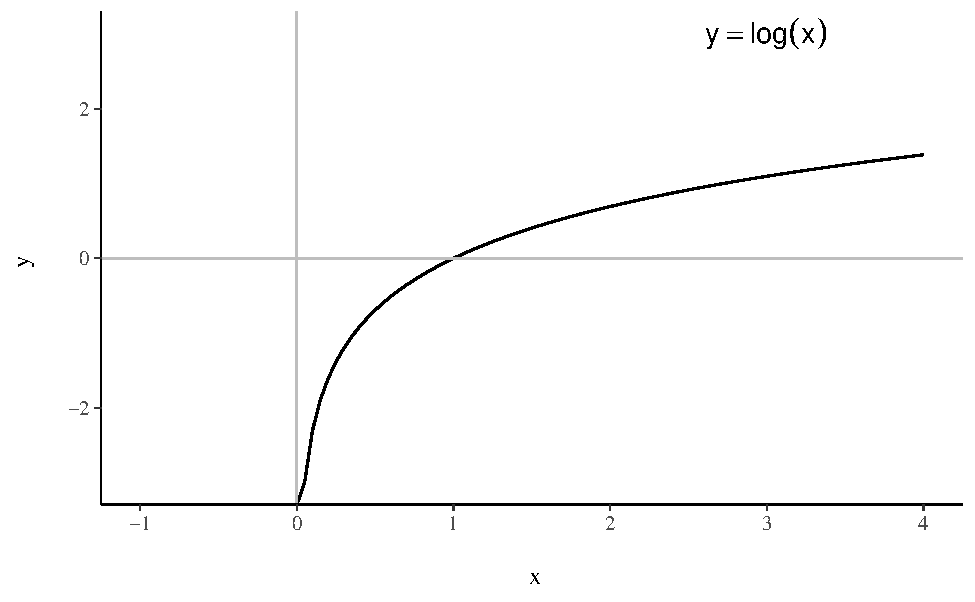
\includegraphics{ds4psy_files/figure-latex/unnamed-chunk-36-1} \end{center}

\hypertarget{gauss-normale}{%
\chapter{La Normale motivata dal metodo dei minimi quadrati}\label{gauss-normale}}

La distribuzione Normale fu scoperta da Gauss nel 1809 e, nella derivazione di Gauss, è intimamente legata al metodo dei minimi quadrati. Vediamo come Gauss arrivò alla definizione della densità Normale.

Tra il 1735 e il 1754 l'Accademia di Francia effettuò quattro misurazioni della lunghezza di un arco di meridiano a latitudini diverse con lo scopo di determinare la figura della Terra.\footnote{L'espressione ``figura della Terra'' è utilizzata in geodesia per indicare la precisione con cui sono definite la dimensione e la forma della Terra.} Papa Benedetto XIV volle contribuire a questo progetto e nel 1750 incaricò Roger Joseph Boscovich (1711---1787) e il gesuita inglese Christopher Maire di misurare un arco di meridiana nei pressi di Roma e contemporaneamente di costruire una nuova mappa dello Stato Pontificio. Il loro rapporto fu pubblicato nel 1755.

La relazione tra lunghezza d'arco e latitudine per archi piccoli è approssimativamente \(y = \alpha + \beta x\), dove \(y\) è la lunghezza dell'arco e \(x = sin^2L\), dove \(L\) è la latitudine del punto medio dell'arco. Il problema di Boscovich era quello di stimare \(\alpha\) e \(\beta\) da cinque osservazioni di \((x, y)\).

Nel 1757 pubblicò una sintesi del rapporto del 1755 in cui proponeva di risolvere il problema di riconciliare le relazioni lineari inconsistenti mediante la minimizzazione della somma dei valori assoluti dei residui, sotto il vincolo che la somma dei residui fosse uguale a zero. In altre parole, Boscovich propose di minimizzare la quantità \(\sum \mid y_i - a - b x_i \mid\) rispetto ad \(a\) e \(b\) sotto il vincolo \((y_i - a - b x_i) = 0\). Boscovich fu il primo a formulare un metodo per adattare una retta ai dati descritti da un diagramma a dispersione, laddove l'orientamento della retta dipende dalla minimizzazione di una funzione dei residui. La formulazione e la soluzione di Boscovich erano puramente verbali ed era accompagnata da un diagramma che spiegava il metodo di minimizzazione.

Nella \emph{Mécanique Céleste}, Laplace (1749, 1827) ritornò sul problema di Boscovich e mostrò in maniera formale come sia possibile minimizzare la quantità \(\sum w_i \mid y_i - a - b x_i \mid\). Il metodo della minimizzazione del valore assoluto degli scarti presentava degli svantaggi rispetto al metodo dei minimi quadrati: (1) la stima della pendenza della retta era complicata da calcolare e (2) il metodo era limitato a una sola variabile indipendente. Il metodo scomparve quindi dalla pratica statistica fino alla seconda metà del XX secolo quando venne riproposto nel contesto della discussione della robustezza delle stime.

In seguito, tale problema venne ripreso da Legendre. Il suo \emph{Nouvelle methods pour la determinazione des orbites des comètes} contiene un'appendice (pp.~72-80) intitolata \emph{Sur la méthode des moindres carrés}, in cui per la prima volta il metodo dei minimi quadrati viene presentato come un metodo algebrico per l'adattamento di un modello lineare ai dati. Legendre scrive \emph{``Tra tutti i princìpi che si possono proporre a questo scopo, credo che non ce ne sia uno più generale, più esatto e più facile da applicare di quello di cui ci siamo serviti nelle precedenti ricerche, e che consiste nel minimizzare la somma dei quadrati degli errori. In questo modo si stabilisce una sorta di equilibrio tra gli errori, che impedisce agli estremi di prevalere e ben si presta a farci conoscere lo stato del sistema più vicino alla verità.''}

La somma dei quadrati degli errori è

\[
\sum_{i=1}^n e_i^2 = (y_i - a - b_1x_{i1} - \dots - b_m x_{im})^2.
\]

Per trovare il minimo di tale funzione, Legendre pone a zero le derivate della funzione rispetto ad \(a, b_1, \dots, b_m\), il che conduce a quelle che in seguito sono state chiamate le ``equazioni normali''. Risolvendo il sistema di equazioni normali rispetto \(a, b_1, \dots, b_m\), si determinano le stime dei minimi quadrati dei parametri del modello di regressione.

Tutto questo è rilevante per la derivazione della Normale perché, in questo contesto, Legendre osservò che la media aritmetica, quale caso speciale dei minimi quadrati, si ottiene minimizzando \(\sum(y_i - b)^2\). In precedenza, Laplace si era posto il problema di mostrare che la media aritmetica è la migliore stima possibile della tendenza centrale di una distribuzione di errori di misurazione, ma non ci era riuscito perché aveva minimizzato il valore assoluto degli scarti, il che portava ad identificare la mediana quale migliore stimatore della tendenza centrale della distribuzione degli errori, non la media.

Nel 1809, Gauss riformulò il problema ponendosi le seguenti domande. Che forma deve avere la densità della distribuzione degli errori? Quale quantità deve essere minimizzata per fare in modo che la media aritmetica risulti la miglior stima possibile della tendenza centrale della distribuzione degli errori? \emph{``Si è soliti considerare come un assioma l'ipotesi che se una qualsiasi grandezza è stata determinata da più osservazioni dirette, fatte nelle stesse circostanze e con uguale cura, la media aritmetica dei valori osservati dà il valore più probabile, se non rigorosamente, eppure con una grade approssimazione, così che è sempre più sicuro utilizzare tale valore.''}

Basandosi sul risultato di Legendre (ovvero, che è necessario minimizzare il quadrato degli scarti dalla tendenza centrale, non il valore assoluto degli scarti), Gauss derivò la formula della densità Normale quale modello teorico della distribuzione degli errori di misurazione. La Normale ha infatti la proprietà desiderata: il valore atteso della distribuzione corrisponde alla media aritmetica.

La scoperta della distribuzione normale segna l'inizio di una nuova era nella statistica. La distribuzione Normale è importante, in primo luogo, perché molti fenomeni naturali hanno approssimativamente le caratteristiche descritte dall'esempio precedente. In secondo luogo, è importante perché molti modelli statistici assumono che il fenomeno aleatorio di interesse abbia una distribuzione Normale.

Nella derivazione della Normale, Gauss fornì una giustificazione probabilistica al metodo dei minimi quadrati basata sull'ipotesi che le osservazioni siano distribuite normalmente e che la distribuzione a priori del parametro di tendenza centrale sia uniforme. Si noti come la discussione sia formulata in termini bayesiani.

La derivazione formale della Normale è troppo complessa per gli scopi presenti. Il Paragrafo \ref{normal-random-walk} illustra invece come si possa giungere alla Normale mediante una simulazione. La motivazione del presente escursus storico è stata quella di mostrare come la Normale sia fortemente legata, in un contesto storico, al modello lineare e al metodo dei minimi quadrati.

\hypertarget{appendix:max-like}{%
\chapter{La stima di massima verosimiglianza}\label{appendix:max-like}}

\hypertarget{la-stima-di-massima-verosimiglianza}{%
\section{La stima di massima verosimiglianza}\label{la-stima-di-massima-verosimiglianza}}

La funzione di verosimiglianza rappresenta la ``credibilità relativa'' dei valori del parametro di interesse. Ma qual è il valore più credibile? Se utilizziamo soltanto la funzione di verosimiglianza, allora la risposta è data dalla stima di massima verosimiglinza.

\begin{definition}
Un valore di \(\theta\) che massimizza \(\mathcal{L}(\theta \mid y)\) sullo spazio parametrico \(\Theta\) è detto \emph{stima di massima verosimiglinza} (s.m.v.) di \(\theta\) ed è indicato con \(\hat{\theta}\):

\begin{equation}
\hat{\theta} = \argmax_{\theta \in \Theta} \mathcal{L}(\theta).
\end{equation}
\end{definition}

Il paradigma frequentista utilizza la funzione di verosimiglianza quale unico strumento per giungere alla stima del valore più credibile del parametro sconosciuto \(\theta\). Tale stima corrisponde al punto di massimo della funzione di verosimiglianza. In base all'approccio bayesiano, invece, il valore più credibile del parametro sconosciuto \(\theta\), anziché alla s.m.v., corrisponde invece alla moda (o media, o mediana) della distribuzione a posteriori \(p(\theta \mid y)\) che si ottiene combinando la verosimiglianza \(p(y \mid \theta)\) con la distribuzione a priori \(p(\theta)\).

\hypertarget{derivation-smv-prop}{%
\section{La s.m.v. per una proporzione}\label{derivation-smv-prop}}

La s.m.v. della proporzione di successi \(\theta\) in una sequenza di prove Bernoulliane è uguale data dalla proporzione di successi campionari. Questo risultato può essere dimostrato come segue.

\begin{proof}
Per \(n\) prove Bernoulliane indipendenti, le quali producono \(y\) successi e (\(n-y\)) insuccessi, la funzione nucleo (ovvero, la funzione di verosimiglianza da cui sono state escluse tutte le costanti moltiplicative che non hanno alcun effetto su \(\hat{\theta}\)) è

\[
\mathcal{L}(p \mid y) = \theta^y (1-\theta)^{n - y}.\notag
\] La funzione nucleo di log-verosimiglianza è

\[
\begin{aligned}
\ell(\theta \mid y) &= \log \mathcal{L}(\theta \mid y) \notag\\
          &= \log \left(\theta^y (1-\theta)^{n - y} \right) \notag\\
          &= \log \theta^y + \log \left( (1-\theta)^{n - y} \right) \notag\\
          &= y \log \theta + (n - y) \log (1-\theta).\notag
\end{aligned}
\]

Per calcolare il massimo della funzione di log-verosimiglianza è necessario differenziare \(\ell(\theta \mid y)\) rispetto a \(\theta\), porre la derivata a zero e risolvere. La derivata di \(\ell(\theta \mid y)\) è:

\[
\ell'(\theta \mid y) = \frac{y}{\theta} -\frac{n-y}{1-\theta}.
\]

Ponendo l'equazione uguale a zero e risolvendo otteniamo la s.m.v.:

\begin{equation}
  \hat{\theta} = \frac{y}{n},
  \label{eq:mlprop}
\end{equation}

ovvero la frequenza relativa dei successi nel campione.
\end{proof}

\hypertarget{calcolo-numerico}{%
\subsection*{Calcolo numerico}\label{calcolo-numerico}}


In maniera più semplice, il risultato descritto nel Paragrafo \ref{derivation-smv-prop} può essere ottenuto mediante una simulazione in \R. Iniziamo a definire un insieme di valori possibili per il parametro incognito \(\theta\):

\begin{Shaded}
\begin{Highlighting}[]
\NormalTok{theta }\OtherTok{\textless{}{-}} \FunctionTok{seq}\NormalTok{(}\DecValTok{0}\NormalTok{, }\DecValTok{1}\NormalTok{, }\AttributeTok{length.out =} \FloatTok{1e3}\NormalTok{)}
\end{Highlighting}
\end{Shaded}

Sappiamo che la funzione di verosimiglianza è la funzione di massa di probabilità espressa in funzione del parametro sconosciuto \(\theta\) assumendo come noti i dati. Questo si può esprimere in \(\R\) nel modo seguente:

\begin{Shaded}
\begin{Highlighting}[]
\NormalTok{like }\OtherTok{\textless{}{-}} \FunctionTok{dbinom}\NormalTok{(}\AttributeTok{x =} \DecValTok{23}\NormalTok{, }\AttributeTok{size =} \DecValTok{30}\NormalTok{, }\AttributeTok{prob =}\NormalTok{ theta)}
\end{Highlighting}
\end{Shaded}

Si noti che, nell'istruzione precedente, abbiamo passato alla funzione \texttt{dbinom()} i dati, ovvero \texttt{x\ =\ 23} successi in \texttt{size\ =\ 30} prove. Inoltre, abbiamo passato alla funzione il vettore \texttt{prob\ =\ theta} che contiene 1000 valori possibili per il parametro \(\theta \in [0, 1]\). Per ciascuno dei valori \(\theta\), la funzione \texttt{dbinom()} ritorna un valore che corrisopnde all'ordinata della funzione di verosimiglianza, tenendo sempre costanti i dati (ovvero, 6 successi in 9 prove). Un grafico della funzione di verosimiglianza è dato da:

\begin{Shaded}
\begin{Highlighting}[]
\FunctionTok{tibble}\NormalTok{(theta, like) }\SpecialCharTok{\%\textgreater{}\%} 
  \FunctionTok{ggplot}\NormalTok{(}\FunctionTok{aes}\NormalTok{(}\AttributeTok{x =}\NormalTok{ theta, }\AttributeTok{y =}\NormalTok{ like)) }\SpecialCharTok{+}
  \FunctionTok{geom\_line}\NormalTok{() }\SpecialCharTok{+}
  \FunctionTok{labs}\NormalTok{(}
    \AttributeTok{y =} \FunctionTok{expression}\NormalTok{(}\FunctionTok{L}\NormalTok{(theta)),}
    \AttributeTok{x =} \FunctionTok{expression}\NormalTok{(}\StringTok{\textquotesingle{}Valori possibili di\textquotesingle{}} \SpecialCharTok{\textasciitilde{}}\NormalTok{ theta)}
\NormalTok{  )}
\end{Highlighting}
\end{Shaded}

\begin{center}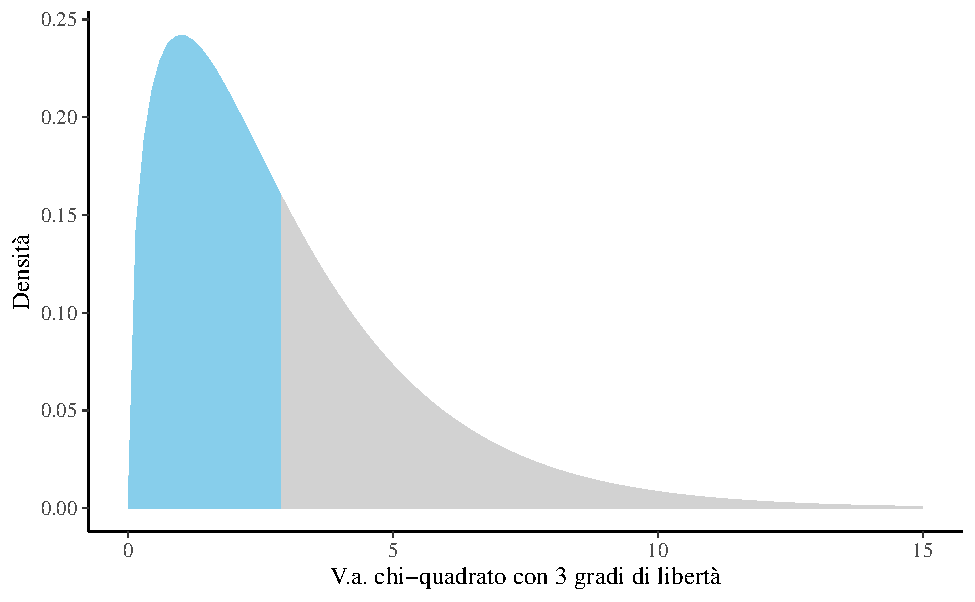
\includegraphics{ds4psy_files/figure-latex/unnamed-chunk-40-1} \end{center}

Nella simulazione, il valore \(\theta\) che massimizza la funzione di verosimiglianza può essere trovato nel modo seguente:

\begin{Shaded}
\begin{Highlighting}[]
\NormalTok{theta[}\FunctionTok{which.max}\NormalTok{(like)]}
\CommentTok{\#\textgreater{} [1] 0.7668}
\end{Highlighting}
\end{Shaded}

Il valore così trovato è uguale al valore definito dalla \eqref{eq:mlprop}.

\hypertarget{derivation-smv-norm}{%
\section{La s.m.v. del modello Normale}\label{derivation-smv-norm}}

Ora che abbiamo capito come costruire la funzione verosimiglianza di una binomiale è relativamente semplice fare un passo ulteriore e considerare la verosimiglianza del caso di una funzione di densità, ovvero nel caso di una variabile casuale continua. Consideriamo qui il caso della Normale.

\begin{proof}
La densità di una distribuzione Normale di parametri \(\mu\) e \(\sigma\) è

\[
f(y \mid \mu, \sigma) = \frac{1}{\sigma \sqrt{2\pi}} \exp\left\{-\frac{1}{2\sigma^2}(y-\mu)^2\right\}.
\label{eq:gausslike}
\]

Poniamoci il problema di trovare la s.m.v. dei parametri sconosciuti \(\mu\) e \(\sigma\) nel caso in cui le \(n\) osservazioni \(y = (y_1, \dots, y_n)\) sono realizzazioni indipendenti ed identicamente distribuite (di seguito, i.i.d.) della medesima variabile casuale \(Y \sim \mathcal{N}(\mu, \sigma)\). Per semplicità, scriveremo \(\theta = \{\mu, \sigma\}.\)

Il campione osservato è un insieme di eventi, ciascuno dei quali corrisponde alla realizzazione di una variabile casuale --- possiamo pensare ad uno di tali eventi come all'estrazione casuale di un valore dalla ``popolazione'' \(\mathcal{N}(\mu, \sigma)\). Se le variabili casuali sono i.i.d., la loro densità congiunta è data da:

\begin{align}
f(y \mid \theta) &= f(y_1 \mid \theta) \cdot f(y_2 \mid \theta) \cdot \; \dots \; \cdot f(y_n \mid \theta)\notag\\
                 &= \prod_{i=1}^n f(y_i \mid \theta),
\label{eq:gauss-prob-cong}
\end{align}

laddove la funzione \(f(\cdot)\) è la \eqref{eq:gausslike}. Tenendo costanti i dati \(y\), la funzione di verosimiglianza è:

\begin{equation}
\mathcal{L}(\theta \mid y) = \prod_{i=1}^n f(y_i \mid \theta).
\label{eq:gausslike2}
\end{equation}

L'obiettivo è quello di massimizzare la funzione di verosimiglianza per trovare i valori \(\theta\) ottimali. Usando la notazione matematica questo si esprime dicendo che cerchiamo l'argmax della \eqref{eq:gausslike2} rispetto a \(\theta\), ovvero

\[
\hat{\theta} = \text{argmax}_{\theta} \prod_{i=1}^n f(y_i \mid \theta).
\]

Questo problema si risolve calcolando le derivate della funzione rispetto a \(\theta\), ponendo le derivate uguali a zero e risolvendo. Saltando tutti i passaggi algebrici di questo procedimento, per \(\mu\) troviamo

\begin{equation}
\hat{\mu} = \frac{1}{n} \sum_{i=1}^n y_i
\label{eq:maxlikemu}
\end{equation}

e per \(\sigma\) abbiamo

\begin{equation}
\hat{\sigma} = \sqrt{\sum_{i=1}^n\frac{1}{n}(y_i- \mu)^2}.
\label{eq:maxlikesigma}
\end{equation}

In altri termini, la s.m.v. del parametro \(\mu\) è la media del campione e la s.m.v. del parametro \(\sigma\) è la deviazione standard del campione.
\end{proof}

\hypertarget{calcolo-numerico-1}{%
\section*{Calcolo numerico}\label{calcolo-numerico-1}}


Consideriamo ora un esempio che utilizza dei dati reali. I dati corrispondono ai valori BDI-II dei trenta soggetti del campione clinico di \citet{zetschefuture2019}:

\begin{Shaded}
\begin{Highlighting}[]
\NormalTok{d }\OtherTok{\textless{}{-}} \FunctionTok{tibble}\NormalTok{(}
  \AttributeTok{y =} \FunctionTok{c}\NormalTok{(}
    \DecValTok{26}\NormalTok{, }\DecValTok{35}\NormalTok{, }\DecValTok{30}\NormalTok{, }\DecValTok{25}\NormalTok{, }\DecValTok{44}\NormalTok{, }\DecValTok{30}\NormalTok{, }\DecValTok{33}\NormalTok{, }\DecValTok{43}\NormalTok{, }\DecValTok{22}\NormalTok{, }\DecValTok{43}\NormalTok{, }\DecValTok{24}\NormalTok{, }\DecValTok{19}\NormalTok{, }\DecValTok{39}\NormalTok{, }\DecValTok{31}\NormalTok{, }\DecValTok{25}\NormalTok{, }
    \DecValTok{28}\NormalTok{, }\DecValTok{35}\NormalTok{, }\DecValTok{30}\NormalTok{, }\DecValTok{26}\NormalTok{, }\DecValTok{31}\NormalTok{, }\DecValTok{41}\NormalTok{, }\DecValTok{36}\NormalTok{, }\DecValTok{26}\NormalTok{, }\DecValTok{35}\NormalTok{, }\DecValTok{33}\NormalTok{, }\DecValTok{28}\NormalTok{, }\DecValTok{27}\NormalTok{, }\DecValTok{34}\NormalTok{, }\DecValTok{27}\NormalTok{, }\DecValTok{22}\NormalTok{)}
\NormalTok{)}
\end{Highlighting}
\end{Shaded}

Ci poniamo l'obiettivo di creare la funzione di verosimiglianza per questi dati, supponendo, in base ai risultati di ricerche precedenti, di sapere che i punteggi BDI-II si distribuiscono secondo una legge Normale.

Per semplificare il problema, assumeremo di conoscere \(\sigma\) (lo porremo uguale alla deviazione standard del campione) in modo da avere un solo parametro sconosciuto, cioè \(\mu\). Il problema è dunque quello di trovare la funzione di verosimiglianza per il parametro \(\mu\), date le 30 osservazioni del campione e dato \(\sigma = s = 6.61\).

Per una singola osservazione, la funzione di verosimiglianza è la densità Normale espressa in funzione dei parametri. Per un campione di osservazioni i.i.d., ovvero \(y = (y_1, y_2, \dots, y_n)\), la verosimiglianza è la funzione di densità congiunta \(f(y \mid \mu, \sigma)\) espressa in funzione dei parametri, ovvero \(\mathcal{L}(\mu, \sigma \mid y)\). Dato che le osservazioni sono i.i.d., la densità congiunta è data dal prodotto delle densità delle singole osservazioni. Per semplicità, assumiamo \(\sigma\) noto e uguale alla deviazione standard del campione:

\begin{Shaded}
\begin{Highlighting}[]
\NormalTok{true\_sigma }\OtherTok{\textless{}{-}} \FunctionTok{sd}\NormalTok{(d}\SpecialCharTok{$}\NormalTok{y)}
\NormalTok{true\_sigma }
\CommentTok{\#\textgreater{} [1] 6.607}
\end{Highlighting}
\end{Shaded}

Avendo posto \(\sigma = 6.61\), per una singola osservazione \(y_i\) abbiamo

\[
f(y_i \mid \mu, \sigma) = \frac{1}{{6.61 \sqrt {2\pi}}}\exp\left\{{-\frac{(y_i - \mu)^2}{2\cdot 6.61^2}}\right\},\notag
\]

dove il pedice \(i\) specifica l'osservazione \(y_i\) tra le molteplici osservazioni \(y\), e \(\mu\) è il parametro sconosciuto che deve essere determinato (nell'esempio, \(\sigma = s\)). La densità congiunta è dunque

\[
f(y \mid \mu, \sigma) = \, \prod_{i=1}^n f(y_i \mid \mu, \sigma)\notag
\] e, alla luce dei dati osservati, la verosimiglianza diventa

\[
\begin{aligned}
\mathcal{L}(\mu, \sigma \mid y) =& \, \prod_{i=1}^n f(y_i \mid \mu, \sigma) = \notag\\
& \frac{1}{{6.61 \sqrt {2\pi}}}\exp\left\{{-\frac{(26 - \mu)^2}{2\cdot 6.61^2}}\right\} \times \notag\\
 & \frac{1}{{6.61 \sqrt {2\pi}}}\exp\left\{{-\frac{(35 - \mu)^2}{2\cdot 6.61^2}}\right\} \times  \notag\\
& \vdots \notag\\
 & \frac{1}{{6.61 \sqrt {2\pi}}}\exp\left\{{-\frac{(22 - \mu)^2}{2\cdot 6.61^2}}\right\}.
\end{aligned}
\label{eq:lldepression}
\]

Poniamoci ora il problema di rappresentare graficamente la funzione di verosimiglianza per il parametro \(\mu\). Avendo un solo parametro sconosciuto, possiamo rappresentare la verosimiglianza con una curva. In \R, definiamo la funzione di log-verosimiglianza nel modo seguente:

\begin{Shaded}
\begin{Highlighting}[]
\NormalTok{log\_likelihood }\OtherTok{\textless{}{-}} \ControlFlowTok{function}\NormalTok{(y, mu, }\AttributeTok{sigma =}\NormalTok{ true\_sigma) \{}
  \FunctionTok{sum}\NormalTok{(}\FunctionTok{dnorm}\NormalTok{(y, mu, sigma, }\AttributeTok{log =} \ConstantTok{TRUE}\NormalTok{))}
\NormalTok{\}}
\end{Highlighting}
\end{Shaded}

Nella funzione \texttt{log\_likelihood()}, \texttt{y} è un vettore che, nel caso presente contiene \(n = 30\) valori. Per ciascuno di questi valori, la funzione \texttt{dnorm()} trova la densità Normale utilizzando il valore \(\mu\) che passato a \texttt{log\_likelihood()} e il valore \(\sigma\) uguale a 6.61 --- nell'esempio, questo parametro viene assunto come noto. L'argomento \texttt{log\ =\ TRUE} specifica che deve essere preso il logaritmo. La funzione \texttt{dnorm()} è un argomento della funzione \texttt{sum()}. Ciò significa che i 30 valori così trovati, espressi su scala logaritmica, verranno sommati --- sommare logaritmi è equivalente a fare il prodotto dei valori sulla scala originaria.

Se applichiamo questa funzione ad un solo valore \(\mu\) otteniamo l'ordinata della funzione di log-verosimiglianza in corrispondenza del valore \(\mu\) (si veda la figura \eqref{eq:lldepression}). Si noti che, per trovare un tale valore, abbiamo utilizzato le seguenti informazioni:

\begin{itemize}
\tightlist
\item
  i 30 dati del campione,
\item
  il valore \(\sigma = s\) fissato a 6.61,
\item
  il singolo valore \(\mu\) passato alla funzione \texttt{log\_likelihood()}.
\end{itemize}

Avendo trovato un singolo punto della funzione di log-verosimiglianza, dobbiamo ripetere i calcoli precedenti per tutti i possibili valori che \(\mu\) può assumere. Nel seguente ciclo \texttt{for()} viene calcolata la log-verosimiglianza di 100,000 valori possibili del parametro \(\mu\):

\begin{Shaded}
\begin{Highlighting}[]
\NormalTok{nrep }\OtherTok{\textless{}{-}} \FloatTok{1e5}
\NormalTok{mu }\OtherTok{\textless{}{-}} \FunctionTok{seq}\NormalTok{(}
  \FunctionTok{mean}\NormalTok{(d}\SpecialCharTok{$}\NormalTok{y) }\SpecialCharTok{{-}} \FunctionTok{sd}\NormalTok{(d}\SpecialCharTok{$}\NormalTok{y), }
  \FunctionTok{mean}\NormalTok{(d}\SpecialCharTok{$}\NormalTok{y) }\SpecialCharTok{+} \FunctionTok{sd}\NormalTok{(d}\SpecialCharTok{$}\NormalTok{y), }
  \AttributeTok{length.out =}\NormalTok{ nrep}
\NormalTok{)}

\NormalTok{ll }\OtherTok{\textless{}{-}} \FunctionTok{rep}\NormalTok{(}\ConstantTok{NA}\NormalTok{, nrep)}
\ControlFlowTok{for}\NormalTok{ (i }\ControlFlowTok{in} \DecValTok{1}\SpecialCharTok{:}\NormalTok{nrep) \{}
\NormalTok{  ll[i] }\OtherTok{\textless{}{-}} \FunctionTok{log\_likelihood}\NormalTok{(d}\SpecialCharTok{$}\NormalTok{y, mu[i], true\_sigma)}
\NormalTok{\}}
\end{Highlighting}
\end{Shaded}

Il vettore \texttt{mu} contiene 100,000 possibili valori del parametro \(\mu\); tali valori sono stati scelti nell'intervallo \(\bar{y} \pm s\). Per ciascuno di questi valori la funzione \texttt{log\_likelihood()} calcola il valore di log-verosimiglianza. I 100,000 risultati vengono salvati nel vettore \texttt{ll}.

I vettori \texttt{mu} e \texttt{ll} possono dunque essere usati per disegnare il grafico della funzione di log-verosimiglianza per il parametro \(\mu\):

\begin{Shaded}
\begin{Highlighting}[]
\FunctionTok{tibble}\NormalTok{(mu, ll) }\SpecialCharTok{\%\textgreater{}\%} 
\FunctionTok{ggplot}\NormalTok{(}\FunctionTok{aes}\NormalTok{(}\AttributeTok{x =}\NormalTok{ mu, }\AttributeTok{y =}\NormalTok{ ll)) }\SpecialCharTok{+}
  \FunctionTok{geom\_line}\NormalTok{() }\SpecialCharTok{+}
  \FunctionTok{vline\_at}\NormalTok{(}\FunctionTok{mean}\NormalTok{(d}\SpecialCharTok{$}\NormalTok{y), }\AttributeTok{color =} \StringTok{"gray"}\NormalTok{, }\AttributeTok{linetype =} \StringTok{"dashed"}\NormalTok{) }\SpecialCharTok{+}
  \FunctionTok{labs}\NormalTok{(}
    \AttributeTok{y =} \StringTok{"Log{-}verosimiglianza"}\NormalTok{,}
    \AttributeTok{x =} \FunctionTok{expression}\NormalTok{(}\StringTok{"Parametro"}\SpecialCharTok{\textasciitilde{}}\NormalTok{mu)}
\NormalTok{  ) }
\end{Highlighting}
\end{Shaded}

\begin{center}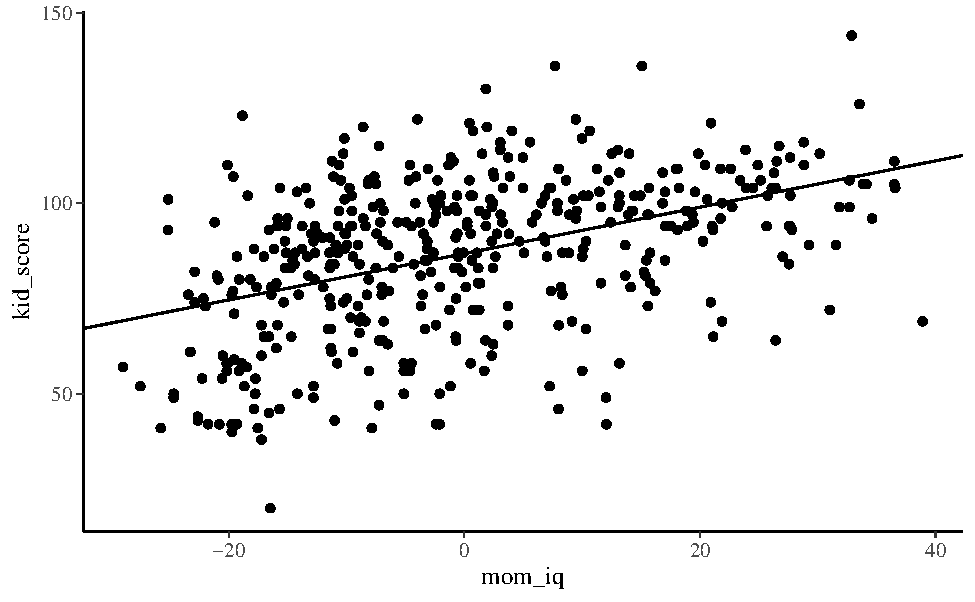
\includegraphics{ds4psy_files/figure-latex/unnamed-chunk-46-1} \end{center}

Dalla figura notiamo che, per i dati osservati, il massimo della funzione di log-verosimiglianza calcolata per via numerica, ovvero 30.93, è identico alla media dei dati campionari e corrisponde al risultato teorico della \eqref{eq:maxlikemu}.

\hypertarget{considerazioni-conclusive}{%
\section*{Considerazioni conclusive}\label{considerazioni-conclusive}}


La verosimiglianza viene utilizzata sia nell'inferenza bayesiana che in quella frequentista. In entrambi i paradigmi di inferenza, il suo ruolo è quantificare la forza con la quale i dati osservati supportano i possibili valori dei parametri sconosciuti.

Nella funzione di verosimiglianza i dati (osservati) vengono trattati come fissi, mentre i valori del parametro (o dei parametri) \(\theta\) vengono variati: la verosimiglianza è una funzione di \(\theta\) per il dato fisso \(y\). Pertanto, la funzione di verosimiglianza riassume i seguenti elementi: un modello statistico che genera stocasticamente i dati (in questo capitolo abbiamo esaminato due modelli statistici: quello binomiale e quello Normale), un intervallo di valori possibili per \(\theta\) e i dati osservati \(y\).

Nella statistica frequentista l'inferenza si basa solo sui dati a disposizione e qualunque informazione fornita dalle conoscenze precedenti non viene presa in considerazione. Nello specifico, nella statistica frequentista l'inferenza viene condotta massimizzando la funzione di (log) verosimiglianza, condizionatamente ai valori assunti dalle variabili casuali campionarie. Nella statistica bayesiana, invece, l'inferenza statistica viene condotta combinando la funzione di verosimiglianza con le distribuzioni a priori dei parametri incogniti \(\theta\).

La differenza fondamentale tra inferenza bayesiana e frequentista è dunque che i frequentisti non ritengono utile descrivere in termini probabilistici i parametri: i parametri dei modelli statistici vengono concepiti come fissi ma sconosciuti. Nell'inferenza bayesiana, invece, i parametri sconosciuti sono intesi come delle variabili casuali e ciò consente di quantificare in termini probabilistici il nostro grado di intertezza relativamente al loro valore.

\hypertarget{appendix:future-exp}{%
\chapter{Le aspettative future dei pazienti depressi}\label{appendix:future-exp}}

\hypertarget{app:zet}{%
\section{\texorpdfstring{La ricerca di \citet{zetschefuture2019}}{La ricerca di @zetschefuture2019}}\label{app:zet}}

Per descrivere vari aspetti dell'analisi bayesiana utilizzeremo dei dati reali, nello specifico quelli raccolti da \citet{zetschefuture2019}. Questi ricercatori si sono chiesti se gli individui depressi manifestino delle aspettative accurate circa il loro umore futuro, oppure se tali aspettative siano distorte negativamente. Esamineremo qui i 30 partecipanti dello studio di \citet{zetschefuture2019} che hanno riportato la presenza di un episodio di depressione maggiore in atto. All'inizio della settimana di test, a questi pazienti è stato chiesto di valutare l'umore che si aspettavano di esperire nei giorni seguenti della settimana. Mediante una app, i partecipanti dovevano poi valutare il proprio umore in cinque momenti diversi di ciascuno dei cinque giorni successivi. Lo studio considera diverse emozioni, ma qui ci concentriamo solo sulla tristezza.

Sulla base dei dati forniti dagli autori, abbiamo calcolato la media dei giudizi relativi al livello di tristezza raccolti da ciascun partecipante tramite la app. Tale media è stata poi sottratta dall'aspettativa del livello di tristezza fornita all'inizio della settimana. La discrepanza tra aspettative e realtà è stata considerata come un evento dicotomico: valori positivi di tale differenza indicano che le aspettative circa il livello di tristezza erano maggiori del livello di tristezza effettivamente esperito --- ciò significa che le aspettative future risultano negativamente distorte (evento codificato con ``1''). Viceversa, si ha che le aspettative risultano positivamente distorte se la differenza descritta in precedenza assume un valore negativo (evento codificato con ``0'').

Nel campione dei 30 partecipanti clinici di \citet{zetschefuture2019}, le aspettative future di 23 partecipanti risultano distorte negativamente e quelle di 7 partecipanti risultano distorte positivamente. Chiameremo \(\theta\) la probabilità dell'evento ``le aspettative del partecipante sono distorte negativamente''. Ci poniamo il problema di ottenere una stima a posteriori di \(\theta\) avendo osservato 23 ``successi'' in 30 prove.

Si noti un punto importante: dire semplicemente che la stima di \(\theta\) è uguale a 23/30 = 0.77 ci porta ad ignorare il livello di incertezza associato a tale stima. Infatti, lo stesso valore (0.77) si può ottenere come 23/30, o 230/300, o 2300/3000, o 23000/30000, ma l'incertezza di una stima pari a 0.77 è molto diversa nei quattro casi. Quando si traggono conclusioni dai dati è invece necessario quantificare il livello della nostra incertezza relativamente alla stima del parametro di interesse (nel caso presente, \(\theta\)). Lo strumento ci consente di quantificare tale incertezza è la distribizione a posteriori \(p(\theta \mid y)\). Ovviamente, \(p(\theta \mid y)\) assume forme molto diverse nei quattro casi descritti sopra.

\hypertarget{appendix:beta-binom}{%
\chapter{Modello Beta-binomiale}\label{appendix:beta-binom}}

\hypertarget{funzione-per-il-modello-beta-binomiale}{%
\section{Funzione per il modello Beta-binomiale}\label{funzione-per-il-modello-beta-binomiale}}

La seguente funzione può essere usata per rappresentare la distribuzione a priori, la distribuzione a posteriori e la versosimiglianza (normalizzata) nel caso del modello Beta-binomiale. I parametri in input sono, nell'ordine, i parametri \(\alpha\) e \(\beta\) della distribuzione a priori Beta, \(y\) (numero di successi) e \(n\) (numero di prove).

\begin{Shaded}
\begin{Highlighting}[]
\NormalTok{plot\_beta\_bin }\OtherTok{\textless{}{-}} \ControlFlowTok{function}\NormalTok{(a, b, y, n) \{}
  \FunctionTok{library}\NormalTok{(}\StringTok{"tidyverse"}\NormalTok{)}
  
\NormalTok{  df1 }\OtherTok{\textless{}{-}} \FunctionTok{data.frame}\NormalTok{(}\AttributeTok{theta =} \FunctionTok{seq}\NormalTok{(}\FloatTok{0.001}\NormalTok{, }\DecValTok{1}\NormalTok{, }\FloatTok{0.001}\NormalTok{))}
\NormalTok{  prior\_un }\OtherTok{\textless{}{-}} \FunctionTok{dbeta}\NormalTok{(df1}\SpecialCharTok{$}\NormalTok{theta, a, b)}
\NormalTok{  df1}\SpecialCharTok{$}\NormalTok{prior }\OtherTok{\textless{}{-}}\NormalTok{ prior\_un }\SpecialCharTok{/} \FunctionTok{sum}\NormalTok{(prior\_un)}

  \CommentTok{\# Likelihood}
\NormalTok{  like\_un }\OtherTok{\textless{}{-}} \FunctionTok{dbinom}\NormalTok{(y, n, }\AttributeTok{prob =} \FunctionTok{seq}\NormalTok{(}\FloatTok{0.001}\NormalTok{, }\DecValTok{1}\NormalTok{, }\FloatTok{0.001}\NormalTok{))}
\NormalTok{  df1}\SpecialCharTok{$}\NormalTok{like }\OtherTok{\textless{}{-}}\NormalTok{ like\_un }\SpecialCharTok{/} \FunctionTok{sum}\NormalTok{(like\_un)}

  \CommentTok{\# Posterior}
\NormalTok{  post\_un }\OtherTok{\textless{}{-}}\NormalTok{ df1}\SpecialCharTok{$}\NormalTok{prior }\SpecialCharTok{*}\NormalTok{ df1}\SpecialCharTok{$}\NormalTok{like}
\NormalTok{  df1}\SpecialCharTok{$}\NormalTok{post }\OtherTok{\textless{}{-}}\NormalTok{ post\_un }\SpecialCharTok{/} \FunctionTok{sum}\NormalTok{(post\_un)}

\NormalTok{  df2 }\OtherTok{\textless{}{-}}\NormalTok{ df1 }\SpecialCharTok{\%\textgreater{}\%}
    \FunctionTok{pivot\_longer}\NormalTok{(}\SpecialCharTok{!}\NormalTok{theta, }\AttributeTok{names\_to =} \StringTok{"grp"}\NormalTok{, }\AttributeTok{values\_to =} \StringTok{"val"}\NormalTok{)}

\NormalTok{  df2}\SpecialCharTok{$}\NormalTok{grp }\OtherTok{\textless{}{-}} \FunctionTok{factor}\NormalTok{(df2}\SpecialCharTok{$}\NormalTok{grp)}
  \CommentTok{\# levels(df2$grp)}
\NormalTok{  df2}\SpecialCharTok{$}\NormalTok{grp }\OtherTok{\textless{}{-}} \FunctionTok{factor}\NormalTok{(df2}\SpecialCharTok{$}\NormalTok{grp, }\AttributeTok{levels =} \FunctionTok{c}\NormalTok{(}\StringTok{"prior"}\NormalTok{, }\StringTok{"like"}\NormalTok{, }\StringTok{"post"}\NormalTok{))}
  \FunctionTok{levels}\NormalTok{(df2}\SpecialCharTok{$}\NormalTok{grp) }\OtherTok{\textless{}{-}}
    \FunctionTok{c}\NormalTok{(}
      \StringTok{"Distribuzione a priori"}\NormalTok{, }\StringTok{"Verosimiglianza"}\NormalTok{,}
      \StringTok{"Distribuzione a posteriori"}
\NormalTok{    )}

\NormalTok{  p }\OtherTok{\textless{}{-}} \FunctionTok{ggplot}\NormalTok{(}\AttributeTok{data =}\NormalTok{ df2) }\SpecialCharTok{+}
    \FunctionTok{geom\_line}\NormalTok{(}\FunctionTok{aes}\NormalTok{(theta, val)) }\SpecialCharTok{+}
    \FunctionTok{facet\_wrap}\NormalTok{(}\SpecialCharTok{\textasciitilde{}}\NormalTok{grp, }\AttributeTok{ncol =} \DecValTok{1}\NormalTok{, }\AttributeTok{scales =} \StringTok{"free\_y"}\NormalTok{) }\SpecialCharTok{+}
    \FunctionTok{coord\_cartesian}\NormalTok{(}\AttributeTok{xlim =} \FunctionTok{c}\NormalTok{(}\DecValTok{0}\NormalTok{, }\DecValTok{1}\NormalTok{)) }\SpecialCharTok{+}
    \FunctionTok{scale\_y\_continuous}\NormalTok{(}\AttributeTok{breaks =} \ConstantTok{NULL}\NormalTok{) }\SpecialCharTok{+}
    \FunctionTok{labs}\NormalTok{(}\AttributeTok{x =} \StringTok{""}\NormalTok{, }\AttributeTok{y =} \StringTok{""}\NormalTok{)}

\NormalTok{  p}
\NormalTok{\}}
\end{Highlighting}
\end{Shaded}

\hypertarget{appendix:const-norm-bino23}{%
\chapter{Verosimiglianza marginale}\label{appendix:const-norm-bino23}}

\hypertarget{derivazione-analitica-della-costante-di-normalizzazione}{%
\section{Derivazione analitica della costante di normalizzazione}\label{derivazione-analitica-della-costante-di-normalizzazione}}

Riportiamo di seguito la derivazione analitica per la costante di normalizzazione discussa nella Sezione \ref{sec:const-normaliz-bino23}, ovvero dell'integrale \eqref{eq:likebino23}.

\begin{proof}
Sia la distribuzione a priori \(\theta \sim \mbox{Beta}(a, b)\) e sia \(y = \{y_1, \dots, y_n\} \sim \Bin(\theta, n)\). Scrivendo la \emph{funzione beta} come

\[
\B(a, b) = \frac{\Gamma(a)\Gamma(b)}{\Gamma(a+b)},
\] la verosimiglianza marginale diventa

\begin{align}
p(y) &= \int p(y \mid \theta) p(\theta) \,\operatorname {d}\!\theta \notag\\
&= \int_0^1 \binom{n}{y}\theta^{y} (1 - \theta)^{n- y} \frac{1}{\B(a,b)} \theta^{a-1} (1-\theta)^{b-1} \,\operatorname {d}\!\theta \notag\\
&= \binom{n}{y}\frac{1}{\B(a,b)} \int_0^1 \theta^{y + a - 1} (1-\theta)^{n- y + b-1}  \,\operatorname {d}\!\theta \notag\\
&= \binom{n}{y}\frac{\Beta(y + a, n- y + b)}{\Beta(a,b)},
\label{eq:constant-norm-beta-binom}
\end{align}

in quanto

\begin{align}
\int_0^1 \frac{1}{\Beta(a,b)} \theta^{a-1} (1-\theta)^{b-1} \,\operatorname {d}\! \theta &= 1\notag\\
\frac{1}{\Beta(a,b)} \int_0^1  \theta^{a-1} (1-\theta)^{b-1} \,\operatorname {d}\! \theta &= 1\notag\\
\int_0^1  \theta^{a-1} (1-\theta)^{b-1} \,\operatorname {d}\!\theta &= \Beta(a,b). \notag
\end{align}

In conclusione, nel caso di una verosimiglianza binomiale \(y = \sim \Bin(\theta, n)\) e di una distribuzione a priori \(\theta \sim \mbox{Beta}(a, b)\), la verosimiglianza marginale diventa uguale alla \eqref{eq:constant-norm-beta-binom}.
\end{proof}

\begin{exercise}

Si verifichi la \eqref{eq:constant-norm-beta-binom} mediante di dati di \citet{zetschefuture2019}.

Per replicare mediante la \eqref{eq:constant-norm-beta-binom} il risultato trovato per via numerica nella Sezione \ref{sec:const-normaliz-bino23} assumiamo una distribuzione a priori uniforme, ovvero \(\mbox{Beta}(1, 1)\). I valori del problema dunque diventano i seguenti:

\begin{Shaded}
\begin{Highlighting}[]
\NormalTok{a }\OtherTok{\textless{}{-}} \DecValTok{1}
\NormalTok{b }\OtherTok{\textless{}{-}} \DecValTok{1}
\NormalTok{y }\OtherTok{\textless{}{-}} \DecValTok{23}
\NormalTok{n }\OtherTok{\textless{}{-}} \DecValTok{30}
\end{Highlighting}
\end{Shaded}

Definiamo

\begin{Shaded}
\begin{Highlighting}[]
\NormalTok{B }\OtherTok{\textless{}{-}} \ControlFlowTok{function}\NormalTok{(a, b) \{}
\NormalTok{  (}\FunctionTok{gamma}\NormalTok{(a) }\SpecialCharTok{*} \FunctionTok{gamma}\NormalTok{(b)) }\SpecialCharTok{/} \FunctionTok{gamma}\NormalTok{(a }\SpecialCharTok{+}\NormalTok{ b)}
\NormalTok{\}}
\end{Highlighting}
\end{Shaded}

Il risultato cercato è

\begin{Shaded}
\begin{Highlighting}[]
\FunctionTok{choose}\NormalTok{(}\DecValTok{30}\NormalTok{, }\DecValTok{23}\NormalTok{) }\SpecialCharTok{*} \FunctionTok{B}\NormalTok{(y }\SpecialCharTok{+}\NormalTok{ a, n }\SpecialCharTok{{-}}\NormalTok{ y }\SpecialCharTok{+}\NormalTok{ b) }\SpecialCharTok{/} \FunctionTok{B}\NormalTok{(a, b)}
\CommentTok{\#\textgreater{} [1] 0.03226}
\end{Highlighting}
\end{Shaded}

\end{exercise}

\hypertarget{es-pratico-zetsche}{%
\chapter{Aspettative degli individui depressi}\label{es-pratico-zetsche}}

Per fare pratica, applichiamo il metodo basato su griglia ad un campione di dati reali. \citet{zetschefuture2019} si sono chiesti se gli individui depressi manifestino delle aspettative accurate circa il loro umore futuro, oppure se tali aspettative siano distorte negativamente. Esamineremo qui i 30 partecipanti dello studio di \citet{zetschefuture2019} che hanno riportato la presenza di un episodio di depressione maggiore in atto. All'inizio della settimana di test, a questi pazienti è stato chiesto di valutare l'umore che si aspettavano di esperire nei giorni seguenti della settimana. Mediante una app, i partecipanti dovevano poi valutare il proprio umore in cinque momenti diversi di ciascuno dei cinque giorni successivi. Lo studio considera diverse emozioni, ma qui ci concentriamo solo sulla tristezza.

Sulla base dei dati forniti dagli autori, abbiamo calcolato la media dei giudizi relativi al livello di tristezza raccolti da ciascun partecipante tramite la app. Tale media è stata poi sottratta dall'aspettativa del livello di tristezza fornita all'inizio della settimana. La discrepanza tra aspettative e realtà è stata considerata come un evento dicotomico: valori positivi di tale differenza indicano che le aspettative circa il livello di tristezza erano maggiori del livello di tristezza effettivamente esperito --- ciò significa che le aspettative future risultano negativamente distorte (evento codificato con ``1''). Viceversa, si ha che le aspettative risultano positivamente distorte se la differenza descritta in precedenza assume un valore negativo (evento codificato con ``0'').

Nel campione dei 30 partecipanti clinici di \citet{zetschefuture2019}, le aspettative future di 23 partecipanti risultano distorte negativamente e quelle di 7 partecipanti risultano distorte positivamente. Chiameremo \(\theta\) la probabilità dell'evento ``le aspettative del partecipante sono distorte negativamente''. Ci poniamo il problema di ottenere una stima a posteriori di \(\theta\) usando il metodo basato su griglia.

\hypertarget{la-griglia}{%
\section{La griglia}\label{la-griglia}}

Fissiamo una griglia di \(n = 50\) valori equispaziati nell'intervallo {[}0, 1{]} per il parametro \(\theta\):

\begin{Shaded}
\begin{Highlighting}[]
\NormalTok{n\_points }\OtherTok{\textless{}{-}} \DecValTok{50}
\NormalTok{p\_grid }\OtherTok{\textless{}{-}} \FunctionTok{seq}\NormalTok{(}\AttributeTok{from =} \DecValTok{0}\NormalTok{, }\AttributeTok{to =} \DecValTok{1}\NormalTok{, }\AttributeTok{length.out =}\NormalTok{ n\_points)}
\NormalTok{p\_grid}
\CommentTok{\#\textgreater{}  [1] 0.00000 0.02041 0.04082 0.06122 0.08163 0.10204}
\CommentTok{\#\textgreater{}  [7] 0.12245 0.14286 0.16327 0.18367 0.20408 0.22449}
\CommentTok{\#\textgreater{} [13] 0.24490 0.26531 0.28571 0.30612 0.32653 0.34694}
\CommentTok{\#\textgreater{} [19] 0.36735 0.38776 0.40816 0.42857 0.44898 0.46939}
\CommentTok{\#\textgreater{} [25] 0.48980 0.51020 0.53061 0.55102 0.57143 0.59184}
\CommentTok{\#\textgreater{} [31] 0.61224 0.63265 0.65306 0.67347 0.69388 0.71429}
\CommentTok{\#\textgreater{} [37] 0.73469 0.75510 0.77551 0.79592 0.81633 0.83673}
\CommentTok{\#\textgreater{} [43] 0.85714 0.87755 0.89796 0.91837 0.93878 0.95918}
\CommentTok{\#\textgreater{} [49] 0.97959 1.00000}
\end{Highlighting}
\end{Shaded}

\hypertarget{distribuzione-a-priori}{%
\section{Distribuzione a priori}\label{distribuzione-a-priori}}

Supponiamo di avere scarse credenze a priori sulla tendenza di un individuo clinicamente depresso a manifestare delle aspettative distorte negativamente circa il suo umore futuro. Imponiamo quindi una distribuzione non informativa sulla distribuzione a priori di \(\theta\) --- ovvero, una distribuzione uniforme nell'intervallo {[}0, 1{]}. Dato che consideriamo soltanto \(n = 50\) valori possibili per il parametro \(\theta\), creiamo un vettore di 50 elementi che conterrà i valori della distribuzione a priori scalando ciascun valore del vettore per \(n\) in modo tale che la somma di tutti i valori sia uguale a 1.0:

\begin{Shaded}
\begin{Highlighting}[]
\NormalTok{prior1 }\OtherTok{\textless{}{-}} \FunctionTok{dbeta}\NormalTok{(p\_grid, }\DecValTok{1}\NormalTok{, }\DecValTok{1}\NormalTok{) }\SpecialCharTok{/} \FunctionTok{sum}\NormalTok{(}\FunctionTok{dbeta}\NormalTok{(p\_grid, }\DecValTok{1}\NormalTok{, }\DecValTok{1}\NormalTok{))}
\NormalTok{prior1}
\CommentTok{\#\textgreater{}  [1] 0.02 0.02 0.02 0.02 0.02 0.02 0.02 0.02 0.02 0.02}
\CommentTok{\#\textgreater{} [11] 0.02 0.02 0.02 0.02 0.02 0.02 0.02 0.02 0.02 0.02}
\CommentTok{\#\textgreater{} [21] 0.02 0.02 0.02 0.02 0.02 0.02 0.02 0.02 0.02 0.02}
\CommentTok{\#\textgreater{} [31] 0.02 0.02 0.02 0.02 0.02 0.02 0.02 0.02 0.02 0.02}
\CommentTok{\#\textgreater{} [41] 0.02 0.02 0.02 0.02 0.02 0.02 0.02 0.02 0.02 0.02}
\end{Highlighting}
\end{Shaded}

Verifichiamo:

\begin{Shaded}
\begin{Highlighting}[]
\FunctionTok{sum}\NormalTok{(prior1)}
\CommentTok{\#\textgreater{} [1] 1}
\end{Highlighting}
\end{Shaded}

\noindent La distribuzione a priori così costruita è rappresentata nella figura \ref{fig:gridappr1}.

\begin{Shaded}
\begin{Highlighting}[]
\NormalTok{p1 }\OtherTok{\textless{}{-}} \FunctionTok{data.frame}\NormalTok{(p\_grid, prior1) }\SpecialCharTok{\%\textgreater{}\%}
  \FunctionTok{ggplot}\NormalTok{(}\FunctionTok{aes}\NormalTok{(}\AttributeTok{x=}\NormalTok{p\_grid, }\AttributeTok{xend=}\NormalTok{p\_grid, }\AttributeTok{y=}\DecValTok{0}\NormalTok{, }\AttributeTok{yend=}\NormalTok{prior1)) }\SpecialCharTok{+}
  \FunctionTok{geom\_line}\NormalTok{() }\SpecialCharTok{+}
  \FunctionTok{geom\_segment}\NormalTok{() }\SpecialCharTok{+}
  \FunctionTok{ylim}\NormalTok{(}\DecValTok{0}\NormalTok{, }\FloatTok{0.17}\NormalTok{) }\SpecialCharTok{+}
  \FunctionTok{labs}\NormalTok{(}
    \AttributeTok{x =} \StringTok{"Parametro \textbackslash{}U03B8"}\NormalTok{,}
    \AttributeTok{y =} \StringTok{"Probabilità a priori"}\NormalTok{,}
    \AttributeTok{title =} \StringTok{"50 punti"}
\NormalTok{  )}
\NormalTok{p1}
\end{Highlighting}
\end{Shaded}

\begin{figure}[h]

{\centering 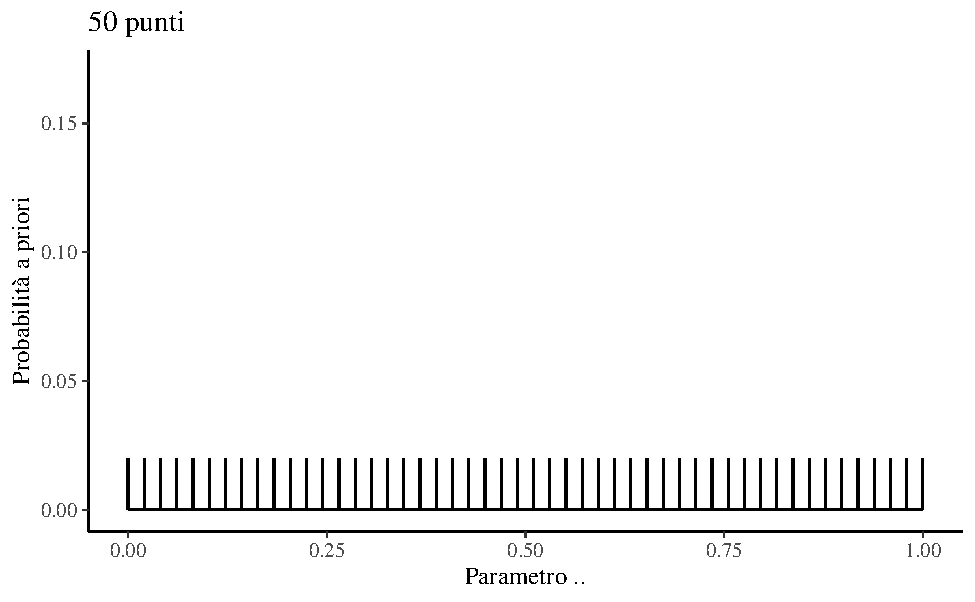
\includegraphics{ds4psy_files/figure-latex/gridappr1-1} 

}

\caption{Rappresentazione grafica della distribuzione a priori per il parametro $   heta$, ovvero la probabilità di aspettative future distorte negativamente.}\label{fig:gridappr1}
\end{figure}

\hypertarget{funzione-di-verosimiglianza}{%
\section{Funzione di verosimiglianza}\label{funzione-di-verosimiglianza}}

Calcoliamo ora la funzione di verosimiglianza utilizzando i 50 valori \(\theta\) definiti in precedenza. A ciascuno dei valori della griglia applichiamo la formula binomiale, tendendo costanti i dati (ovvero 23 ``successi'' in 30 prove). Ad esempio, in corrispondenza del valore \(\theta = 0.816\), l'ordinata della funzione di verosimiglianza diventa

\begin{equation}
\binom{30}{23} \cdot 0.816^{23} \cdot (1 - 0.816)^{7} = 0.135.\notag
\end{equation}

Per \(\theta = 0.837\), l'ordinata della funzione di verosimiglianza sarà

\begin{equation}
\binom{30}{23} \cdot 0.837^{23} \cdot (1 - 0.837)^{7} = 0.104.\notag
\end{equation}

Dobbiamo svolgere questo calcolo per tutti gli elementi della griglia. Usando \(\R\), tale risultato si trova nel modo seguente:

\begin{Shaded}
\begin{Highlighting}[]
\NormalTok{likelihood }\OtherTok{\textless{}{-}} \FunctionTok{dbinom}\NormalTok{(}\AttributeTok{x =} \DecValTok{23}\NormalTok{, }\AttributeTok{size =} \DecValTok{30}\NormalTok{, }\AttributeTok{prob =}\NormalTok{ p\_grid)}
\NormalTok{likelihood}
\CommentTok{\#\textgreater{}  [1] 0.000e+00 2.353e{-}33 1.703e{-}26 1.644e{-}22 1.054e{-}19}
\CommentTok{\#\textgreater{}  [6] 1.525e{-}17 8.602e{-}16 2.528e{-}14 4.607e{-}13 5.819e{-}12}
\CommentTok{\#\textgreater{} [11] 5.499e{-}11 4.106e{-}10 2.520e{-}09 1.311e{-}08 5.919e{-}08}
\CommentTok{\#\textgreater{} [16] 2.362e{-}07 8.457e{-}07 2.749e{-}06 8.197e{-}06 2.260e{-}05}
\CommentTok{\#\textgreater{} [21] 5.799e{-}05 1.393e{-}04 3.149e{-}04 6.721e{-}04 1.359e{-}03}
\CommentTok{\#\textgreater{} [26] 2.612e{-}03 4.779e{-}03 8.340e{-}03 1.390e{-}02 2.214e{-}02}
\CommentTok{\#\textgreater{} [31] 3.372e{-}02 4.910e{-}02 6.830e{-}02 9.068e{-}02 1.147e{-}01}
\CommentTok{\#\textgreater{} [36] 1.378e{-}01 1.568e{-}01 1.682e{-}01 1.689e{-}01 1.575e{-}01}
\CommentTok{\#\textgreater{} [41] 1.349e{-}01 1.044e{-}01 7.133e{-}02 4.166e{-}02 1.973e{-}02}
\CommentTok{\#\textgreater{} [46] 6.937e{-}03 1.535e{-}03 1.473e{-}04 1.868e{-}06 0.000e+00}
\end{Highlighting}
\end{Shaded}

La funzione \texttt{dbinom(x,\ size,\ prob)} richiede che vengano specificati tre parametri: il numero di ``successi'', il numero di prove e la probabilità di successo. Nella chiamata precedente, \texttt{x} (numero di successi) e \texttt{size} (numero di prove bernoulliane) sono degli scalari e \texttt{prob} è il vettore \texttt{p\_grid}. In tali circostanze, l'output di \texttt{dbinom()} è il vettore che abbiamo chiamato \texttt{likelihood}. Gli elementi di tale vettore sono stati calcolati applicando la formula della distribuzione binomiale a ciascuno dei 50 elementi della griglia, tenendo sempre costanti i dati {[}ovvero, \texttt{x} (il numero di successi) e \texttt{size} (numero di prove bernoulliane){]}; ciò che varia è il valore \texttt{prob}, che assume valori diversi (\texttt{p\_grid}) in ciascuna cella della griglia.

La chiamata a \texttt{dbinom()} produce dunque un vettore i cui valori corrispondono all'ordinata della funzione di verosimiglianza per per ciascun valore \(\theta\) specificato in \texttt{p\_grid}. La verosimiglianza discretizzata così ottenuta è riportata nella figura \ref{fig:gridappr2}.

\begin{Shaded}
\begin{Highlighting}[]
\NormalTok{p2 }\OtherTok{\textless{}{-}} \FunctionTok{data.frame}\NormalTok{(p\_grid, likelihood) }\SpecialCharTok{\%\textgreater{}\%}
  \FunctionTok{ggplot}\NormalTok{(}\FunctionTok{aes}\NormalTok{(}\AttributeTok{x=}\NormalTok{p\_grid, }\AttributeTok{xend=}\NormalTok{p\_grid, }\AttributeTok{y=}\DecValTok{0}\NormalTok{, }\AttributeTok{yend=}\NormalTok{likelihood)) }\SpecialCharTok{+}
  \FunctionTok{geom\_segment}\NormalTok{() }\SpecialCharTok{+}
  \FunctionTok{ylim}\NormalTok{(}\DecValTok{0}\NormalTok{, }\FloatTok{0.17}\NormalTok{) }\SpecialCharTok{+}
  \FunctionTok{labs}\NormalTok{(}
    \AttributeTok{x =} \StringTok{"Parametro \textbackslash{}U03B8"}\NormalTok{,}
    \AttributeTok{y =} \StringTok{"Verosimiglianza"}
\NormalTok{  )}
\NormalTok{p2}
\end{Highlighting}
\end{Shaded}

\begin{figure}[h]

{\centering 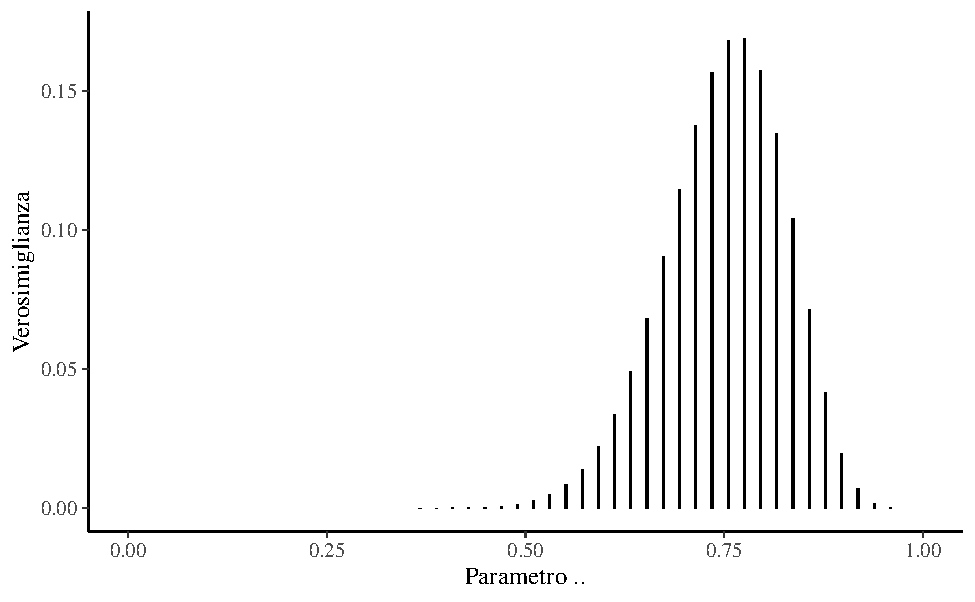
\includegraphics{ds4psy_files/figure-latex/gridappr2-1} 

}

\caption{Rappresentazione della funzione di verosimiglianza per il parametro $\theta$, ovvero la probabilità di aspettative future distorte negativamente.}\label{fig:gridappr2}
\end{figure}

\hypertarget{distribuzione-a-posteriori-1}{%
\section{Distribuzione a posteriori}\label{distribuzione-a-posteriori-1}}

L'approssimazione discretizzata della distribuzione a posteriori \(p(\theta \mid y)\) si ottiene facendo il prodotto della verosimiglianza e della distribuzione a priori per poi scalare tale prodotto per una costante di normalizzazione. Il prodotto \(p(\theta)\mathcal{L}(y \mid \theta)\) produce la distribuzione a posteriori \emph{non standardizzata}.

Nel caso di una distribuzione a priori non informativa (ovvero una distribuzione uniforme), per ottenere la funzione a posteriori non standardizzata è sufficiente moltiplicare ciascun valore della funzione di verosimiglianza per 0.02. Per esempio, per il primo valore della funzione di verosimiglianza usato quale esempio poco sopra, abbiamo \(0.135 \cdot 0.02\); per il secondo valore dell'esempio abbiamo \(0.104 \cdot 0.02\); e così via. Possiamo svolgere tutti i calcoli usando \(\R\) nel modo seguente:\footnote{Ricordiamo il principio dell'aritmetica vettorializzata: i vettori \texttt{likelihood} e \texttt{prior1} sono entrambi costituiti da 50 elementi. Se facciamo il prodotto tra i due vettori otteniamo un vettore di 50 elementi, ciascuno dei quali uguale al prodotto dei corrispondenti elementi dei vettori \texttt{likelihood} e \texttt{prior1}.}

\begin{Shaded}
\begin{Highlighting}[]
\NormalTok{unstd\_posterior }\OtherTok{\textless{}{-}}\NormalTok{ likelihood }\SpecialCharTok{*}\NormalTok{ prior1}
\NormalTok{unstd\_posterior}
\CommentTok{\#\textgreater{}  [1] 0.000e+00 4.705e{-}35 3.406e{-}28 3.288e{-}24 2.107e{-}21}
\CommentTok{\#\textgreater{}  [6] 3.050e{-}19 1.720e{-}17 5.057e{-}16 9.214e{-}15 1.164e{-}13}
\CommentTok{\#\textgreater{} [11] 1.100e{-}12 8.211e{-}12 5.040e{-}11 2.622e{-}10 1.184e{-}09}
\CommentTok{\#\textgreater{} [16] 4.724e{-}09 1.691e{-}08 5.499e{-}08 1.639e{-}07 4.519e{-}07}
\CommentTok{\#\textgreater{} [21] 1.160e{-}06 2.786e{-}06 6.297e{-}06 1.344e{-}05 2.718e{-}05}
\CommentTok{\#\textgreater{} [26] 5.224e{-}05 9.558e{-}05 1.668e{-}04 2.780e{-}04 4.428e{-}04}
\CommentTok{\#\textgreater{} [31] 6.744e{-}04 9.820e{-}04 1.366e{-}03 1.814e{-}03 2.294e{-}03}
\CommentTok{\#\textgreater{} [36] 2.756e{-}03 3.136e{-}03 3.363e{-}03 3.378e{-}03 3.150e{-}03}
\CommentTok{\#\textgreater{} [41] 2.697e{-}03 2.087e{-}03 1.427e{-}03 8.331e{-}04 3.945e{-}04}
\CommentTok{\#\textgreater{} [46] 1.387e{-}04 3.070e{-}05 2.947e{-}06 3.736e{-}08 0.000e+00}
\end{Highlighting}
\end{Shaded}

Avendo calcolato i valori della funzione a posteriori non standardizzata è poi necessario dividere per una costante di normalizzazione. Nel caso discreto, trovare il denominatore del teorema di Bayes è facile: esso è uguale alla somma di tutti i valori della distribuzione a posteriori non normalizzata. Per i dati presenti, tale costante di normalizzazione è uguale a 0.032:

\begin{Shaded}
\begin{Highlighting}[]
\FunctionTok{sum}\NormalTok{(unstd\_posterior)}
\CommentTok{\#\textgreater{} [1] 0.03161}
\end{Highlighting}
\end{Shaded}

La standardizzazione dei due valori usati come esempio è data da: \(0.135 \cdot 0.02 / 0.032\) e da \(0.104 \cdot 0.02 / 0.032\). Usiamo \(\R\) per svolgere questo calcolo su tutti i 50 valori di \texttt{unstd\_posterior} così che la somma dei 50 i valori di \texttt{posterior} sia uguale a 1.0:

\begin{Shaded}
\begin{Highlighting}[]
\NormalTok{posterior }\OtherTok{\textless{}{-}}\NormalTok{ unstd\_posterior }\SpecialCharTok{/} \FunctionTok{sum}\NormalTok{(unstd\_posterior)}
\NormalTok{posterior}
\CommentTok{\#\textgreater{}  [1] 0.000e+00 1.488e{-}33 1.077e{-}26 1.040e{-}22 6.666e{-}20}
\CommentTok{\#\textgreater{}  [6] 9.649e{-}18 5.442e{-}16 1.600e{-}14 2.915e{-}13 3.681e{-}12}
\CommentTok{\#\textgreater{} [11] 3.479e{-}11 2.597e{-}10 1.594e{-}09 8.295e{-}09 3.745e{-}08}
\CommentTok{\#\textgreater{} [16] 1.494e{-}07 5.350e{-}07 1.739e{-}06 5.186e{-}06 1.430e{-}05}
\CommentTok{\#\textgreater{} [21] 3.669e{-}05 8.814e{-}05 1.992e{-}04 4.252e{-}04 8.599e{-}04}
\CommentTok{\#\textgreater{} [26] 1.652e{-}03 3.023e{-}03 5.276e{-}03 8.794e{-}03 1.401e{-}02}
\CommentTok{\#\textgreater{} [31] 2.133e{-}02 3.106e{-}02 4.321e{-}02 5.737e{-}02 7.256e{-}02}
\CommentTok{\#\textgreater{} [36] 8.719e{-}02 9.922e{-}02 1.064e{-}01 1.069e{-}01 9.966e{-}02}
\CommentTok{\#\textgreater{} [41] 8.533e{-}02 6.602e{-}02 4.513e{-}02 2.635e{-}02 1.248e{-}02}
\CommentTok{\#\textgreater{} [46] 4.389e{-}03 9.712e{-}04 9.321e{-}05 1.182e{-}06 0.000e+00}
\end{Highlighting}
\end{Shaded}

Verifichiamo:

\begin{Shaded}
\begin{Highlighting}[]
\FunctionTok{sum}\NormalTok{(posterior)}
\CommentTok{\#\textgreater{} [1] 1}
\end{Highlighting}
\end{Shaded}

La distribuzione a posteriori così trovata non è altro che la versione normalizzata della funzione di verosimiglianza: questo avviene perché la distribuzione a priori uniforme non ha aggiunto altre informazioni oltre a quelle che erano già fornite dalla funzione di verosimiglianza. L'approssimazione discretizzata di \(p(\theta \mid y)\) che abbiamo appena trovato è riportata nella figura \ref{fig:gridappr3}.

\begin{Shaded}
\begin{Highlighting}[]
\NormalTok{p3 }\OtherTok{\textless{}{-}} \FunctionTok{data.frame}\NormalTok{(p\_grid, posterior) }\SpecialCharTok{\%\textgreater{}\%}
  \FunctionTok{ggplot}\NormalTok{(}\FunctionTok{aes}\NormalTok{(}\AttributeTok{x=}\NormalTok{p\_grid, }\AttributeTok{xend=}\NormalTok{p\_grid, }\AttributeTok{y=}\DecValTok{0}\NormalTok{, }\AttributeTok{yend=}\NormalTok{posterior)) }\SpecialCharTok{+}
  \FunctionTok{geom\_segment}\NormalTok{() }\SpecialCharTok{+}
  \FunctionTok{ylim}\NormalTok{(}\DecValTok{0}\NormalTok{, }\FloatTok{0.17}\NormalTok{) }\SpecialCharTok{+}
  \FunctionTok{labs}\NormalTok{(}
    \AttributeTok{x =} \StringTok{"Parametro \textbackslash{}U03B8"}\NormalTok{,}
    \AttributeTok{y =} \StringTok{"Probabilità a posteriori"}
\NormalTok{  )}
\NormalTok{p3}
\end{Highlighting}
\end{Shaded}

\begin{figure}[h]

{\centering 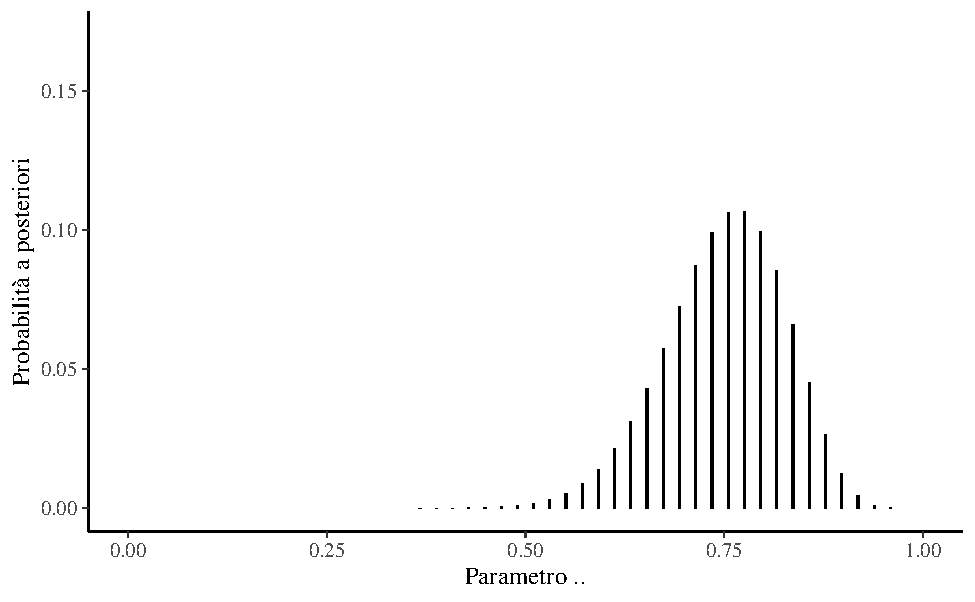
\includegraphics{ds4psy_files/figure-latex/gridappr3-1} 

}

\caption{Rappresentazione della distribuzione a posteriori per il parametro $\theta$, ovvero la probabilità di aspettative future distorte negativamente.}\label{fig:gridappr3}
\end{figure}

I grafici delle figure \ref{fig:gridappr1}, \ref{fig:gridappr2} e \ref{fig:gridappr3} sono state calcolati utilizzando una griglia di 50 valori equi-spaziati per il parametro \(\theta\). I segmenti verticali rappresentano l'intensità della funzione in corrispondenza di ciascuna modalità parametro \(\theta\). Nella figura \ref{fig:gridappr1} e nella figura \ref{fig:gridappr3} la somma delle lunghezze dei segmenti verticali è uguale a 1.0; ciò non si verifica, invece, nel caso della figura \ref{fig:gridappr3} (la funzione di verosimiglianza non è mai una funzione di probabilità, né nel caso discreto né in quello continuo).

\hypertarget{es-depression-beta-2-10}{%
\section{La stima della distribuzione a posteriori (versione 2)}\label{es-depression-beta-2-10}}

Continuiamo l'analisi di questi dati esaminiamo l'impatto di una distribuzione a priori informativa sulla distribuzione a posteriori. Una distribuzione a priori informativa riflette un alto grado di certezza a priori sui valori dei parametri del modello. Un ricercatore utilizza una distribuzione a priori informativa per introdurre nel processo di stima informazioni pre-esistenti alla raccolta dei dati, introducendo così delle restrizioni sulla possibile gamma di valori del parametro.

Nel caso presente, supponiamo che la letteratura psicologica fornisca delle informazioni su \(\theta\) (la probabilità che le aspettative future di un individuo clinicamente depresso siano distorte negativamente). Per fare un esempio, supponiamo (irrealisticamente) che tali conoscenze pregresse possano essere rappresentate da una Beta di parametri \(\alpha = 2\) e \(\beta = 10\). Tali ipotetiche conoscenze pregresse ritengono molto plausibili valori \(\theta\) bassi e considerano implausibili valori \(\theta > 0.5\). Questo è equivalente a dire che ci aspettiamo che le aspettative relative all'umore futuro siano distorte negativamente solo per pochissimi individui clinicamente depressi --- ovvero, ci aspettiamo che la maggioranza degli individui clinicamente depressi sia inguaribilmente ottimista. Questa è, ovviamente, una credenza a priori del tutto irrealistica. La esamino qui, non perché abbia alcun senso nel contesto dei dati di \citet{zetschefuture2019}, ma soltanto per fare un esempio nel quale risulta chiaro come la distribuzione a posteriori sia una sorta di ``compromesso'' tra la distribuzione a priori e la verosimiglianza.

Con calcoli del tutto simili a quelli descritti sopra si giunge alla distribuzione a posteriori rappresentata nella figura \ref{fig:gridappr4}. Useremo ora una griglia di 100 valori per il parametro \(\theta\):

\begin{Shaded}
\begin{Highlighting}[]
\NormalTok{n\_points }\OtherTok{\textless{}{-}} \DecValTok{100}
\NormalTok{p\_grid }\OtherTok{\textless{}{-}} \FunctionTok{seq}\NormalTok{(}\AttributeTok{from =} \DecValTok{0}\NormalTok{, }\AttributeTok{to =} \DecValTok{1}\NormalTok{, }\AttributeTok{length.out =}\NormalTok{ n\_points)}
\end{Highlighting}
\end{Shaded}

Per la distribuzione a priori scegliamo una Beta(2, 10):

\begin{Shaded}
\begin{Highlighting}[]
\NormalTok{alpha }\OtherTok{\textless{}{-}} \DecValTok{2}
\NormalTok{beta }\OtherTok{\textless{}{-}} \DecValTok{10}
\NormalTok{prior2 }\OtherTok{\textless{}{-}} \FunctionTok{dbeta}\NormalTok{(p\_grid, alpha, beta) }\SpecialCharTok{/} \FunctionTok{sum}\NormalTok{(}\FunctionTok{dbeta}\NormalTok{(p\_grid, alpha, beta))}
\FunctionTok{sum}\NormalTok{(prior2)}
\CommentTok{\#\textgreater{} [1] 1}
\end{Highlighting}
\end{Shaded}

Tale distribuzione a priori è rappresentata nella figura \ref{fig:gridappr4}:

\begin{Shaded}
\begin{Highlighting}[]
\NormalTok{plot\_df }\OtherTok{\textless{}{-}} \FunctionTok{data.frame}\NormalTok{(p\_grid, prior2)}
\NormalTok{p4 }\OtherTok{\textless{}{-}}\NormalTok{ plot\_df }\SpecialCharTok{\%\textgreater{}\%}
  \FunctionTok{ggplot}\NormalTok{(}\FunctionTok{aes}\NormalTok{(}\AttributeTok{x=}\NormalTok{p\_grid, }\AttributeTok{xend=}\NormalTok{p\_grid, }\AttributeTok{y=}\DecValTok{0}\NormalTok{, }\AttributeTok{yend=}\NormalTok{prior2)) }\SpecialCharTok{+}
  \FunctionTok{geom\_segment}\NormalTok{() }\SpecialCharTok{+}
  \FunctionTok{ylim}\NormalTok{(}\DecValTok{0}\NormalTok{, }\FloatTok{0.17}\NormalTok{) }\SpecialCharTok{+}
  \FunctionTok{labs}\NormalTok{(}
    \AttributeTok{x =} \StringTok{""}\NormalTok{,}
    \AttributeTok{y =} \StringTok{"Probabilità a priori"}
\NormalTok{  )}
\NormalTok{p4}
\end{Highlighting}
\end{Shaded}

\begin{figure}[h]

{\centering 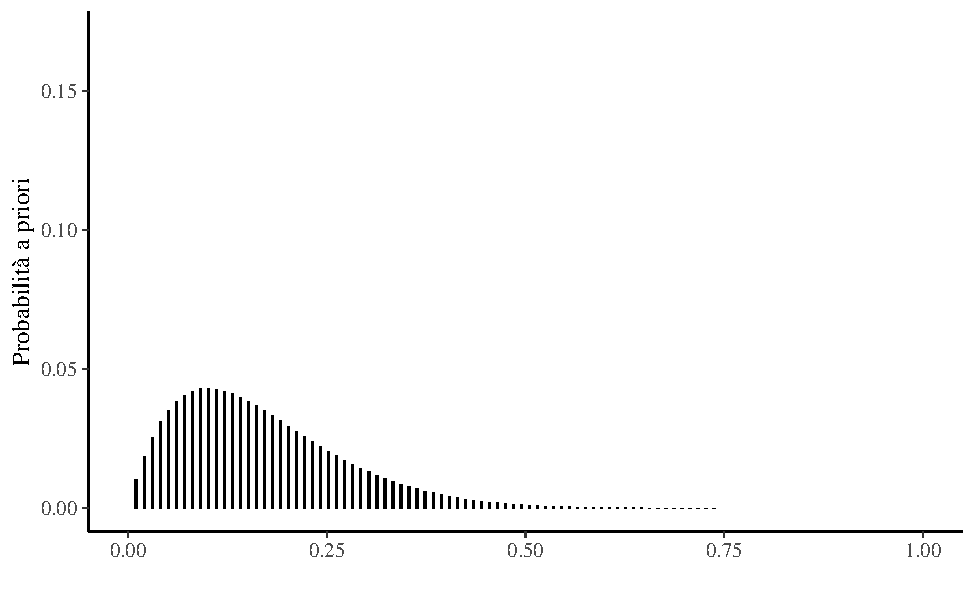
\includegraphics{ds4psy_files/figure-latex/gridappr4-1} 

}

\caption{Rappresentazione di una funzione a priori informativa per il parametro $\theta$.}\label{fig:gridappr4}
\end{figure}

Calcoliamo il valore di verosimiglianza per ciascun punto della griglia:

\begin{Shaded}
\begin{Highlighting}[]
\NormalTok{likelihood }\OtherTok{\textless{}{-}} \FunctionTok{dbinom}\NormalTok{(}\DecValTok{23}\NormalTok{, }\AttributeTok{size =} \DecValTok{30}\NormalTok{, }\AttributeTok{prob =}\NormalTok{ p\_grid)}
\end{Highlighting}
\end{Shaded}

\noindent Per ciascun punto della griglia, il prodotto tra la verosimiglianza e distribuzione a priori è dato da:

\begin{Shaded}
\begin{Highlighting}[]
\NormalTok{unstd\_posterior2 }\OtherTok{\textless{}{-}}\NormalTok{ likelihood }\SpecialCharTok{*}\NormalTok{ prior2}
\end{Highlighting}
\end{Shaded}

\noindent È necessario normalizzare la distribuzione a posteriori discretizzata:

\begin{Shaded}
\begin{Highlighting}[]
\NormalTok{posterior2 }\OtherTok{\textless{}{-}}\NormalTok{ unstd\_posterior2 }\SpecialCharTok{/} \FunctionTok{sum}\NormalTok{(unstd\_posterior2)}
\end{Highlighting}
\end{Shaded}

\noindent Verifichiamo:

\begin{Shaded}
\begin{Highlighting}[]
\FunctionTok{sum}\NormalTok{(posterior2)}
\CommentTok{\#\textgreater{} [1] 1}
\end{Highlighting}
\end{Shaded}

\noindent La nuova funzione a posteriori discretizzata è rappresentata nella figura \ref{fig:gridappr5}:

\begin{Shaded}
\begin{Highlighting}[]
\NormalTok{plot\_df }\OtherTok{\textless{}{-}} \FunctionTok{data.frame}\NormalTok{(p\_grid, posterior2)}
\NormalTok{p5 }\OtherTok{\textless{}{-}}\NormalTok{ plot\_df }\SpecialCharTok{\%\textgreater{}\%}
  \FunctionTok{ggplot}\NormalTok{(}\FunctionTok{aes}\NormalTok{(}\AttributeTok{x =}\NormalTok{ p\_grid, }\AttributeTok{xend =}\NormalTok{ p\_grid, }\AttributeTok{y =} \DecValTok{0}\NormalTok{, }\AttributeTok{yend =}\NormalTok{ posterior2)) }\SpecialCharTok{+}
  \FunctionTok{geom\_segment}\NormalTok{() }\SpecialCharTok{+}
  \FunctionTok{ylim}\NormalTok{(}\DecValTok{0}\NormalTok{, }\FloatTok{0.17}\NormalTok{) }\SpecialCharTok{+}
  \FunctionTok{labs}\NormalTok{(}
    \AttributeTok{x =} \StringTok{"Parametro \textbackslash{}U03B8"}\NormalTok{,}
    \AttributeTok{y =} \StringTok{"Probabilità a posteriori"}
\NormalTok{  )}
\NormalTok{p5}
\end{Highlighting}
\end{Shaded}

\begin{figure}[h]

{\centering 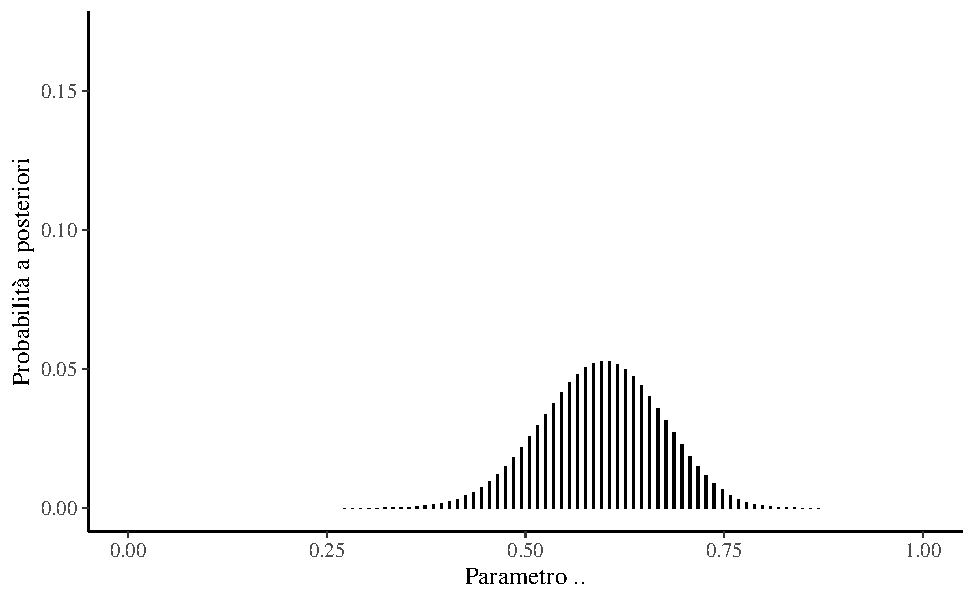
\includegraphics{ds4psy_files/figure-latex/gridappr5-1} 

}

\caption{Rappresentazione della funzione a posteriori per il parametro $\theta$ calcolata utilizzando una distribuzione a priori informativa.}\label{fig:gridappr5}
\end{figure}

Facendo un confronto tra le figure \ref{fig:gridappr4} e \ref{fig:gridappr5} notiamo una notevole differenza tra la distribuzione a priori e la distribuzione a posteriori. In particolare, la distribuzione a posteriori risulta spostata verso destra su posizioni più vicine a quelle della verosimiglianza {[}figura \ref{fig:gridappr2}{]}. Si noti inoltre che, a causa dell'effetto della distribuzione a priori, le distribuzioni a posteriori delle figure \ref{fig:gridappr3} e \ref{fig:gridappr5} sono molto diverse tra loro.

Campioniamo ora 10,000 punti dall'approssimazione discretizzata della distribuzione a posteriori:

\begin{Shaded}
\begin{Highlighting}[]
\CommentTok{\# Set the seed}
\FunctionTok{set.seed}\NormalTok{(}\DecValTok{84735}\NormalTok{)}

\NormalTok{df }\OtherTok{\textless{}{-}} \FunctionTok{data.frame}\NormalTok{(}
\NormalTok{  p\_grid,}
\NormalTok{  posterior2}
\NormalTok{)}
\CommentTok{\# Step 4: sample from the discretized posterior}
\NormalTok{post\_samples }\OtherTok{\textless{}{-}}\NormalTok{ df }\SpecialCharTok{\%\textgreater{}\%}
  \FunctionTok{slice\_sample}\NormalTok{(}
  \AttributeTok{n =} \FloatTok{1e5}\NormalTok{,}
  \AttributeTok{weight\_by =}\NormalTok{ posterior2,}
  \AttributeTok{replace =} \ConstantTok{TRUE}
\NormalTok{)}
\end{Highlighting}
\end{Shaded}

\noindent Una rappresentazione grafica del campione casuale estratto dalla distribuzione a posteriori \(p(\theta \mid y)\) è data da:

\begin{Shaded}
\begin{Highlighting}[]
\NormalTok{post\_samples }\SpecialCharTok{\%\textgreater{}\%}
  \FunctionTok{ggplot}\NormalTok{(}\FunctionTok{aes}\NormalTok{(}\AttributeTok{x =}\NormalTok{ p\_grid)) }\SpecialCharTok{+}
  \FunctionTok{geom\_histogram}\NormalTok{(}
    \FunctionTok{aes}\NormalTok{(}\AttributeTok{y =}\NormalTok{ ..density..), }
    \AttributeTok{color =} \StringTok{"white"}\NormalTok{, }
    \AttributeTok{binwidth =} \FloatTok{0.05}
\NormalTok{  ) }\SpecialCharTok{+}
  \FunctionTok{stat\_function}\NormalTok{(}\AttributeTok{fun =}\NormalTok{ dbeta, }\AttributeTok{args =} \FunctionTok{list}\NormalTok{(}\DecValTok{25}\NormalTok{, }\DecValTok{17}\NormalTok{)) }\SpecialCharTok{+}
  \FunctionTok{lims}\NormalTok{(}\AttributeTok{x =} \FunctionTok{c}\NormalTok{(}\DecValTok{0}\NormalTok{, }\DecValTok{1}\NormalTok{))}
\end{Highlighting}
\end{Shaded}

\begin{center}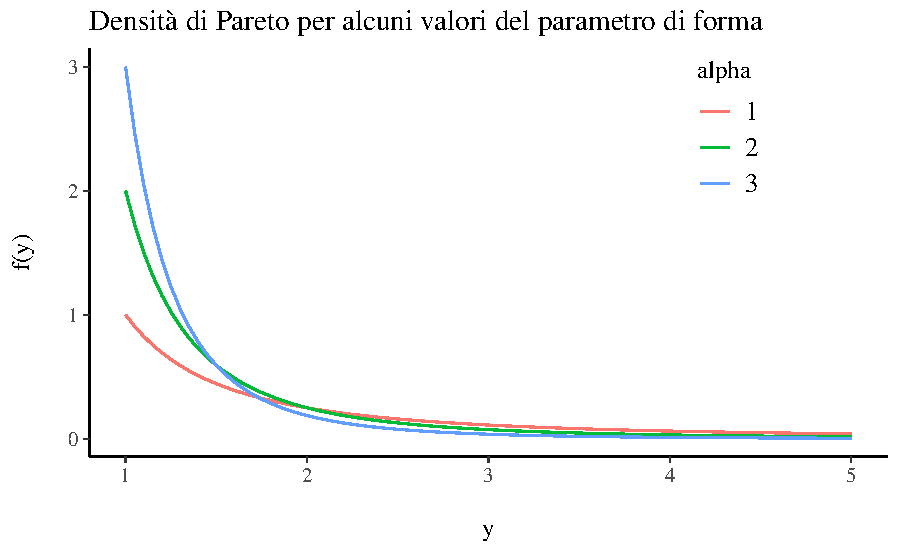
\includegraphics{ds4psy_files/figure-latex/unnamed-chunk-69-1} \end{center}

\noindent All'istogramma è stata sovrapposta la corretta distribuzione a posteriori, ovvero una Beta di parametri 25 (\(y + \alpha\) = 23 + 2) e 17 (\(n - y + \beta\) = 30 - 23 + 10).

La stima della moda a posteriori si ottiene con

\begin{Shaded}
\begin{Highlighting}[]
\NormalTok{df}\SpecialCharTok{$}\NormalTok{p\_grid[}\FunctionTok{which.max}\NormalTok{(df}\SpecialCharTok{$}\NormalTok{posterior2)]}
\CommentTok{\#\textgreater{} [1] 0.596}
\end{Highlighting}
\end{Shaded}

e corrisponde a

\[
\Mo = \frac{\alpha -1}{\alpha + \beta - 2} = \frac{25 - 1}{25 + 17 - 2} = 0.6.
\]

La stima della media a posteriori si ottiene con

\begin{Shaded}
\begin{Highlighting}[]
\FunctionTok{mean}\NormalTok{(post\_samples}\SpecialCharTok{$}\NormalTok{p\_grid)}
\CommentTok{\#\textgreater{} [1] 0.5953}
\end{Highlighting}
\end{Shaded}

e corrisponde a

\[
\bar{\theta} = \frac{\alpha}{\alpha + \beta} = \frac{25}{25 + 17} \approx 0.5952.
\]

La stima della mediana a posteriori si ottiene con

\begin{Shaded}
\begin{Highlighting}[]
\FunctionTok{median}\NormalTok{(post\_samples}\SpecialCharTok{$}\NormalTok{p\_grid)}
\CommentTok{\#\textgreater{} [1] 0.596}
\end{Highlighting}
\end{Shaded}

e corrisponde a

\[
\Me = \frac{\alpha - \frac{1}{3}}{\alpha + \beta - \frac{2}{3}} \approx 0.5968.
\]

\hypertarget{es-pratico-zetsche-funzioni}{%
\section{Versione 2}\label{es-pratico-zetsche-funzioni}}

Possiamo semplificare i calcoli precedenti definendo le funzioni \texttt{likelihood()}, \texttt{prior()} e \texttt{posterior()}.

Per calcolare la funzione di verosimiglianza per i 30 valori di \citet{zetschefuture2019} useremo la funzione \texttt{likelihood()}:

\begin{Shaded}
\begin{Highlighting}[]
\NormalTok{x }\OtherTok{\textless{}{-}} \DecValTok{23}
\NormalTok{N }\OtherTok{\textless{}{-}} \DecValTok{30}
\NormalTok{param }\OtherTok{\textless{}{-}} \FunctionTok{seq}\NormalTok{(}\DecValTok{0}\NormalTok{, }\DecValTok{1}\NormalTok{, }\AttributeTok{length.out =} \DecValTok{100}\NormalTok{)}

\NormalTok{likelihood }\OtherTok{\textless{}{-}} \ControlFlowTok{function}\NormalTok{(param, }\AttributeTok{x =} \DecValTok{23}\NormalTok{, }\AttributeTok{N =} \DecValTok{30}\NormalTok{) \{}
  \FunctionTok{dbinom}\NormalTok{(x, N, param)}
\NormalTok{\}}

\FunctionTok{tibble}\NormalTok{(}
  \AttributeTok{x =}\NormalTok{ param, }
  \AttributeTok{y =} \FunctionTok{likelihood}\NormalTok{(param)}
\NormalTok{) }\SpecialCharTok{\%\textgreater{}\%}
  \FunctionTok{ggplot}\NormalTok{(}\FunctionTok{aes}\NormalTok{(x, y)) }\SpecialCharTok{+}
  \FunctionTok{geom\_line}\NormalTok{() }\SpecialCharTok{+}
  \FunctionTok{labs}\NormalTok{(}
    \AttributeTok{x =} \FunctionTok{expression}\NormalTok{(theta),}
    \AttributeTok{y =} \StringTok{"Verosimiglianza"}
\NormalTok{  )}
\end{Highlighting}
\end{Shaded}

\begin{center}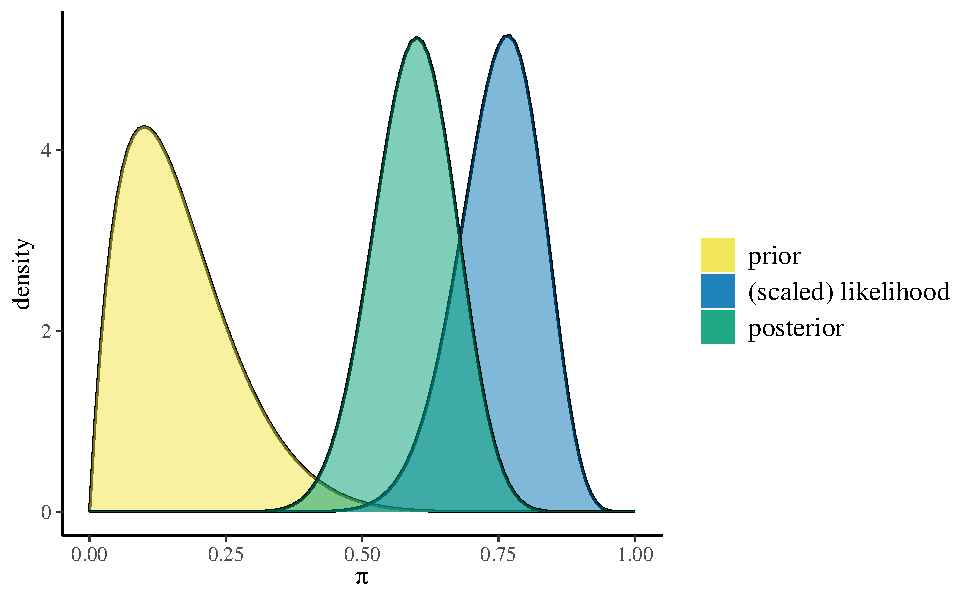
\includegraphics{ds4psy_files/figure-latex/unnamed-chunk-73-1} \end{center}

La funzione \texttt{likelihood()} ritorna l'ordinata della verosimiglianza binomiale per ciascun valore del vettore \texttt{param} in input.

Quale distribuzione a priori utilizzeremo una \(\mbox{Beta}(2, 10)\) che è implementata nella funzione \texttt{prior()}:

\begin{Shaded}
\begin{Highlighting}[]
\NormalTok{prior }\OtherTok{\textless{}{-}} \ControlFlowTok{function}\NormalTok{(param, }\AttributeTok{alpha =} \DecValTok{2}\NormalTok{, }\AttributeTok{beta =} \DecValTok{10}\NormalTok{) \{}
\NormalTok{  param\_vals }\OtherTok{\textless{}{-}} \FunctionTok{seq}\NormalTok{(}\DecValTok{0}\NormalTok{, }\DecValTok{1}\NormalTok{, }\AttributeTok{length.out =} \DecValTok{100}\NormalTok{)}
  \FunctionTok{dbeta}\NormalTok{(param, alpha, beta) }\CommentTok{\# / sum(dbeta(param\_vals, alpha, beta))}
\NormalTok{\}}

\FunctionTok{tibble}\NormalTok{(}
  \AttributeTok{x =}\NormalTok{ param, }
  \AttributeTok{y =} \FunctionTok{prior}\NormalTok{(param)}
\NormalTok{) }\SpecialCharTok{\%\textgreater{}\%}
  \FunctionTok{ggplot}\NormalTok{(}\FunctionTok{aes}\NormalTok{(x, y)) }\SpecialCharTok{+}
  \FunctionTok{geom\_line}\NormalTok{() }\SpecialCharTok{+}
  \FunctionTok{labs}\NormalTok{(}
    \AttributeTok{x =} \FunctionTok{expression}\NormalTok{(theta),}
    \AttributeTok{y =} \StringTok{"Densità"}
\NormalTok{  )}
\end{Highlighting}
\end{Shaded}

\begin{center}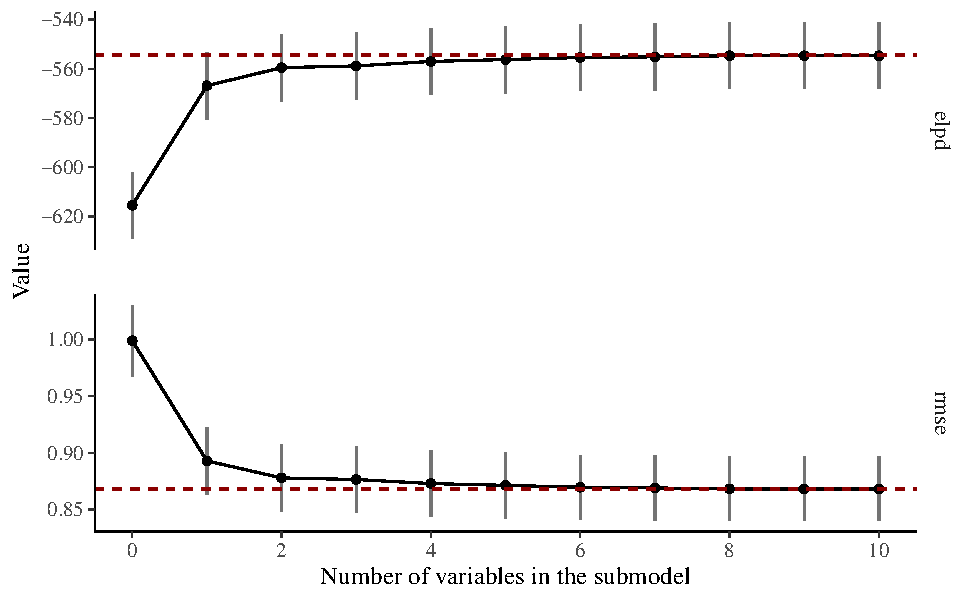
\includegraphics{ds4psy_files/figure-latex/unnamed-chunk-74-1} \end{center}

La funzione \texttt{posterior()} ritorna il prodotto della densità a priori e della verosimiglianza:

\begin{Shaded}
\begin{Highlighting}[]
\NormalTok{posterior }\OtherTok{\textless{}{-}} \ControlFlowTok{function}\NormalTok{(param) \{}
  \FunctionTok{likelihood}\NormalTok{(param) }\SpecialCharTok{*} \FunctionTok{prior}\NormalTok{(param)}
\NormalTok{\}}

\FunctionTok{tibble}\NormalTok{(}
  \AttributeTok{x =}\NormalTok{ param, }
  \AttributeTok{y =} \FunctionTok{posterior}\NormalTok{(param)}
\NormalTok{) }\SpecialCharTok{\%\textgreater{}\%}
  \FunctionTok{ggplot}\NormalTok{(}\FunctionTok{aes}\NormalTok{(x, y)) }\SpecialCharTok{+}
  \FunctionTok{geom\_line}\NormalTok{() }\SpecialCharTok{+}
  \FunctionTok{labs}\NormalTok{(}
    \AttributeTok{x =} \FunctionTok{expression}\NormalTok{(theta),}
    \AttributeTok{y =} \StringTok{"Densità"}
\NormalTok{  )}
\end{Highlighting}
\end{Shaded}

\begin{center}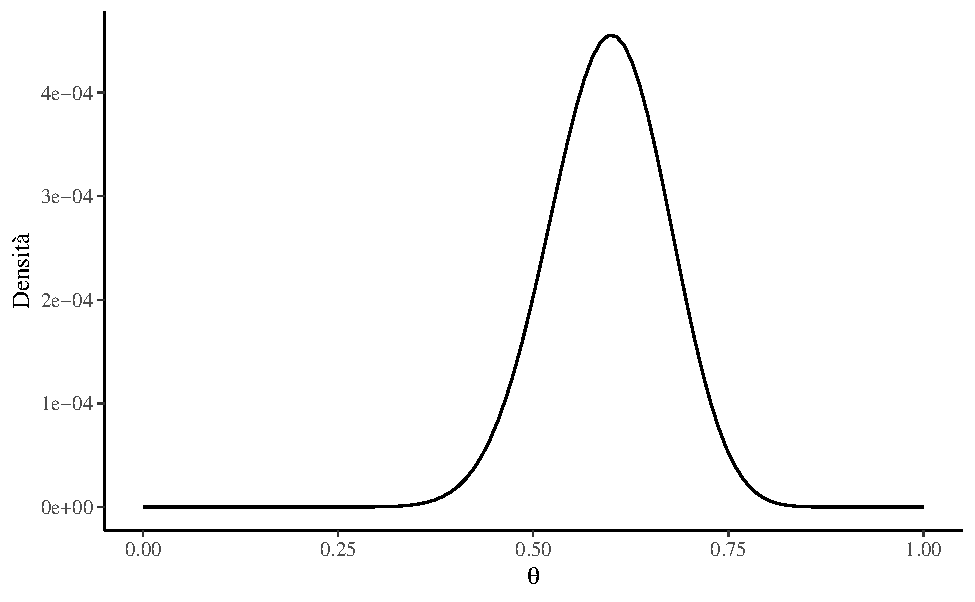
\includegraphics{ds4psy_files/figure-latex/unnamed-chunk-75-1} \end{center}

La distribuzione a posteriori non normalizzata mostrata nella figura replica il risultato ottenuto con il codice utilizzato nella prima parte di questo Capitolo. Per l'implementazione dell'algoritmo di Metropolis non è necessaria la normalizzazione della distribuzione a posteriori.

  \bibliography{refs.bib,book.bib,packages.bib}

\printindex

\end{document}
